\documentclass[12pt]{article}
\usepackage[ngerman]{babel}
\usepackage[utf8]{inputenc}
\usepackage[T1]{fontenc}
\usepackage{graphicx}
\usepackage[hidelinks]{hyperref}
\usepackage[a4paper, lmargin={4cm}, rmargin={2cm}, tmargin={2.5cm}, bmargin={2.5cm}]{geometry}
\usepackage{enumerate}
\usepackage{amssymb}
\usepackage{amsthm}
\usepackage{amsmath}
\usepackage{faktor}
\usepackage{dsfont}
\usepackage{pdfpages}

\graphicspath{ {images/} }

\usepackage{csquotes}
\usepackage{biblatex}
\addbibresource{chapters/bachelor_sources.bib}

\newtheorem{theorem}{Satz}[section]
\newtheorem{corollary}{Korollar}[theorem]
\newtheorem{proposition}[theorem]{Proposition}
\newtheorem{lemma}[theorem]{Lemma}
\newtheorem{example}[theorem]{Beispiel}
\theoremstyle{definition}
\newtheorem{definition}[theorem]{Definition}
\newtheorem{remark}[theorem]{Bemerkung}


\DeclareMathOperator{\ip}{ip}
\DeclareMathOperator{\cpl}{Cpl}
\newcommand{\cplc}{\cpl_{\operatorname{c}}}
\newcommand{\cplbc}{\cpl_{\operatorname{bc}}}
\DeclareMathOperator{\uf}{uf}
\DeclareMathOperator{\id}{id}
\DeclareMathOperator{\CFP}{CFP}
\DeclareMathOperator{\FP}{FP}
\DeclareMathOperator{\AF}{AF}
\DeclareMathOperator{\depth}{depth}
\DeclareMathOperator{\pj}{pj}
\DeclareMathOperator{\pp}{pp}
\DeclareMathOperator{\ST}{ST}
\DeclareMathOperator{\clip}{clip}
\begin{document}
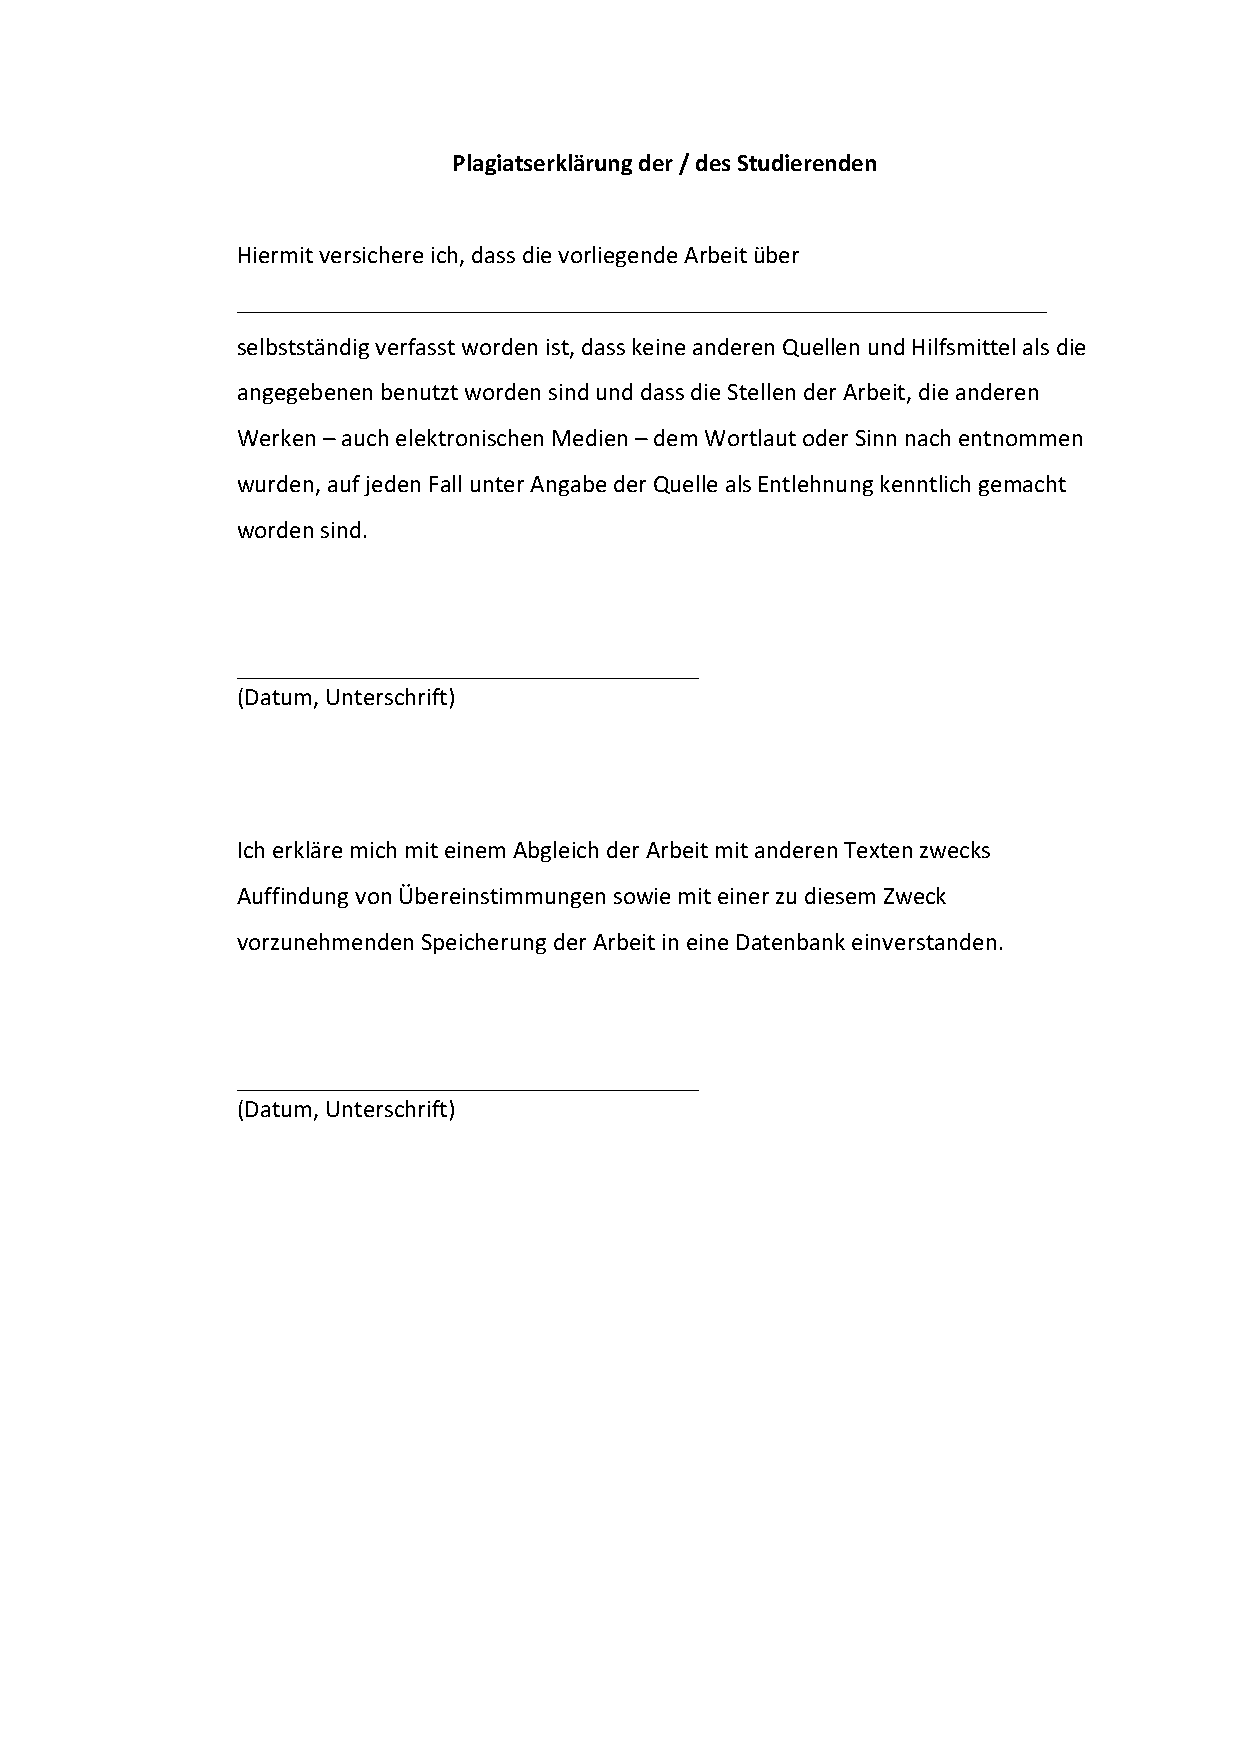
\includepdf{plagiatserklarung_margin.pdf}
%\begin{titlepage}
%\title{
    %{Adaptierte Wasserstein Metrik} \\
    %{Westfälische Wilhelms-Universität}
%}

%\author{Kilian Mandon}
%\date{\today}

%\end{titlepage}

\begin{titlepage}
    \begin{figure}[t]
        \includegraphics[width=0.3\textwidth]{images/Logo_WWU_Münster.png}
    \end{figure}
   \begin{center}
        \vspace*{1cm}
       \textbf{\huge Der Raum der adaptierten stochastischen Prozesse}
       \paragraph{}$~~$\\
       \paragraph{}$~~$\\
       \paragraph{}$~~$\\
       \textbf{neunwöchige Abschlussarbeit im Rahmen der Prüfung} \\ \textbf{im Studiengang der Mathematik (B.Sc.)} \\ \textbf{an der Universität Münster}
       \paragraph{}$~~$\\
       \paragraph{}$~~$\\
       \paragraph{}$~~$\\
       \text{vorgelegt am: \today} \\
       \text{von: Kilian Mandon} \\
       \text{1. Gutachter: Prof. Dr. Martin Huesmann} \\
       \paragraph{}$~~$\\
       \text{Universität Münster}
            
   \end{center}
\end{titlepage}

\tableofcontents
\clearpage

\section{Einleitung}\label{ch:introduction}
Diese Arbeit bespricht die \emph{adaptierte Wasserstein-Metrik} wie sie von Daniel Bartl, Mathias Beiglböck und Gudmund Pammer in \cite{main_paper} vorgestellt wurde. Die adaptierte Wasserstein-Metrik $\mathcal{AW}_p$ ist eine Metrik auf dem Raum adaptierter stochastischer Prozesse $\FP_p$, die nicht nur die Verteilung, sondern auch die Filtration der Prozesse berücksichtigt. Für viele wichtige Operationen der Wahrscheinlichkeitstheorie wie die Doob-Zerlegung, Optimal-Stopping-Probleme oder Martingale ist die Berücksichtigung der gegebenen Filtration essentiell. Die adaptierte Wasserstein-Metrik kann diesen Anspruch in vielen Punkten erfüllen, so zeigen wir etwa in Abschnitt \ref{ch:topological_properties} die Stetigkeit der Doob-Zerlegung und die Stetigkeit des Ertrags eines Optimal-Stopping-Problems. 

Die Arbeit beginnt mit einer ausführlichen Vorstellung der Grundlagen für die adaptierte Wasserstein-Metrik. Kapitel \ref{ch:basics} bespricht die klassische Wasserstein-Metrik, bedingte Erwartungen und Verteilungen sowie die Eigenschaft der Bikausalität von Kopplungen. Es werden viele kleinere Aussagen gemacht, die für die übrige Arbeit wichtig sind.

Die Kapitel \ref{ch:wasserstein_space}, \ref{ch:adapted_functions} und \ref{ch:topological_properties} erarbeiten die wichtigsten Aussagen des zugrundeliegenden Papers \cite{main_paper} und stellen die Beweise in ausführlicherer Form dar. In Kapitel \ref{ch:wasserstein_space} wird ein polnischer Raum $(\mathcal{Z}_1, d)$ konstruiert, sodass $(\FP_p, \mathcal{AW}_p)$ isomorph zu $\mathcal{P}_p(\mathcal{Z}_1)$ mit der klassischen Wasserstein-Metrik ist. In Kapitel \ref{ch:adapted_functions} werden die \emph{adaptierten Funktionen} vorgestellt, die für adaptierte stochastische Prozesse separierend wirken: Zwei Prozesse $\mathbb{X,Y}$ sind genau dann gleich bezüglich der adaptierten Wasserstein-Metrik, wenn die Erwartungswerte $\mathbb{E}(f(\mathbb{X}))$ und $\mathbb{E}(f(\mathbb{Y}))$ für alle adaptierten Funktionen $f$ übereinstimmen. In Kapitel \ref{ch:topological_properties} werden wichtige geometrische und topologische Eigenschaften der adaptierten Wasserstein-Metrik hergeleitet. Es wird gezeigt, dass eine Familie $(\mathbb{X}_i)_{i\in I}$ genau dann relativ kompakt ist, wenn die Verteilungen $(\mathcal{L}(X_i))_{i\in I}$ relativ kompakt bezüglich der Wasserstein-Metrik sind, das heißt wenn $(\mathcal{L}(X_i))_{i\in I}$ straff und uniform $p$-integrierbar sind. Außerdem wird die Stetigkeit von wichtigen Operationen wie der Doob-Zerlegung und Optimal-Stopping gezeigt, sowie die Eigenschaft, dass $\FP_p$ ein geodätischer Raum ist.

Zusätzlich zur Vorstellung dieser Ergebnisse des Papers werden als eigene Resultate in Proposition \ref{thm:awp_convergence_char} die Konvergenz bezüglich $\mathcal{AW}_p$ charakterisiert und in Kapitel \ref{ch:implementation} der Fall von endlichen Wahrscheinlichkeitsräumen betrachtet, in welchem die adaptierte Wasserstein-Metrik mit Methoden der linearen Programmierung berechnet werden kann.

\section{Grundlagen}\label{ch:basics}
\subsection{Notation}
Für den Verlauf dieser Arbeit fixieren wir einen Zeit-Horizont $N \in \mathbb{N}$ und $p \in [1,\infty)$. Für $1\leq t \leq N$ sei $\mathcal{X}_t$ ein polnischer Raum mit einer kompatiblen Metrik $d_{\mathcal{X}_t}$. Für Mengen $\left(A_{i}\right)_{s\leq i \leq r}$ kürzen wir das kartesische Produkt ab durch
$$A_{s:r} := A_s \times ... \times A_r$$
Mit dieser Notation schreiben wir $\mathcal{X}:=\mathcal{X}_{1:N}$.

Für einen polnischen Raum $A$ mit kompatibler Metrik $d_A$ betrachten wir zwei Räume von Maßen: $\mathcal{P}(A)$, den Raum der Borel-Wahrscheinlichkeitsmaße auf $A$, und die Teilmenge $\mathcal{P}_p(A) \subset \mathcal{P}(A)$ der Wahrscheinlichkeitsmaße mit endlichem $p$-ten Moment, das heißt
$$\int d_A^p(a_0, x) \mu(dx) < \infty$$
für ein fixes (und damit für alle) $a_0 \in A$. Für zwei Wahrscheinlichkeitsmaße $\mu \in \mathcal{P}(A), \nu \in \mathcal{P}(B)$ schreiben wir $\cpl(\mu, \nu)$ für die Menge aller \emph{Kopplungen} von $\mu$ und $\nu$, das heißt Maße $\pi \in \mathcal{P}(A \times B)$ mit $\pi(\cdot, B)\equiv \mu$ und $\pi(A, \cdot)=\nu$.

\subsection{Wasserstein-Distanz}
\begin{definition}[Wasserstein-Distanz]\label{def:wasserstein_distance}
    Sei $A$ polnisch mit einer fixierten kompatiblen Metrik $d_A$. Die $p$-te Wasserstein"=Distanz zwischen zwei Wahrscheinlichkeitsmaßen $\mu, \nu \in \mathcal{P}_p(A)$ ist definiert als
    $$\mathcal{W}_p(\mu, \nu) := \left( \inf_{\pi \in \cpl(\mu, \nu)} \int d^p_A(x, y) \pi(dx, dy) \right)^\frac{1}{p}$$
\end{definition}
Wir versehen $\mathcal{P}(A)$ mit der Topologie von schwacher Konvergenz, das heißt eine Basis der Topologie sind Mengen $\{U_{f, x, r} \vert f \in C_b(A), x\in \mathbb{R}, r>0\}$ der Form 
$$U_{f, x, r} = \left\{ \mu \in \mathcal{P}(A) \vert \left| \int f d\mu - x\right| < r\right\}$$
Bezüglich dieser Topologie betrachten wir auf $\mathcal{P}(A)$ die Borel $\sigma$"=Algebra. Auf $\mathcal{P}_p(A)$ ist die Topologie induziert durch $\mathcal{W}_p$, und auch hier betrachten wir die assoziierte Borel $\sigma$-Algebra.
\begin{lemma}\label{thm:closed_couplings}
Seien $\mathcal{A,B}$ polnische Räume. Dann gilt: 
\begin{enumerate}
    \item Für $(\mu_n)_{n\in \mathbb{N}} \subset\mathcal{P}(A), \mu_n \rightarrow \mu \in \mathcal{P}(A)$ ist der Grenzwert eindeutig.
    \item Für $(\pi_n) \subset \mathcal{P}(\mathcal{A} \times \mathcal{B}), \pi_n \rightarrow \pi$ schwach konvergieren auch die Marginalien von $\pi_n$ schwach gegen die von $\pi$. 
    \item Für $\mu \in \mathcal{P}(\mathcal{A}), \nu \in \mathcal{P}(\mathcal{B})$ ist $\cpl(\mu, \nu)$ abgeschlossen.
\end{enumerate}
\end{lemma}
\begin{proof}
    Seien $\mu, \tilde{\mu}$ zwei Grenzwerte von $(\mu_n)$ in schwacher Konvergenz. Sei $E \subseteq \mathcal{A}$ abgeschlossen. Für $m \in \mathbb{N}$ betrachte die stetige Funktion 
    $$f_m: x \mapsto (1-m\cdot d(x,E)) \vee 0$$
    $f_m$ ist stetig und beschränkt, also gilt 
    $$\lim_{n \rightarrow \infty} \mu_n(f_m) = \mu(f_m) = \tilde{\mu}(f_m)$$
    Es konvergiert $f_m \rightarrow \mathds{1}_E$ fast sicher dominiert durch $1$, somit gilt also auch $\mu(E) =\tilde{\mu}(E)$. Da abgeschlossene Mengen ein $\cap$-stabiler Erzeuger sind, folgt $\mu=\tilde{\mu}$ und damit die erste Behauptung.

    Sei $(\pi_n)_{n\in\mathbb{N}} \subset \mathcal{P}(\mathcal{A}\times\mathcal{B})$ eine Folge und konvergent gegen $\pi$. Wir schreiben $\mu_n, \nu_n$ bzw. $\mu, \nu$ für die Marginalien von $\pi_n$ bzw. $\pi$. Sei $f\in C_b(\mathcal{A})$. Wir können $f \in C_b(\mathcal{A}\times\mathcal{B})$ auffassen als $x,y\mapsto f(x)$. Da $f$ stetig und beschränkt ist, gilt 
    $$\mu(f) = \pi(f) = \lim_{n\rightarrow \infty} \pi_n(f) = \lim_{n\rightarrow\infty} \mu_n(f)$$ 
    Daraus folgt die zweite Behauptung.

    Für eine Folge von Kopplungen $(\pi_n)_{n\in\mathbb{N}} \subset \cpl(\mu,\nu)$ konvergent gegen $\pi$ müssen also auch die Marginalien von $pi_n$ gegen die von $\pi$ konvergieren. Die Marginalien sind aber konstant $\mu$ und $\nu$, und wegen der Eindeutigkeit des Grenzwertes nach dem ersten Punkt gilt $\pi \in \cpl(\mu,\nu)$.
\end{proof}
\begin{lemma}\label{thm:optimal_coupling}
In \ref{def:wasserstein_distance} wird dass Infimum tatsächlich angenommen, das heißt es existiert ein $\pi \in \cpl(\mu, \nu)$, sodass
$$\mathcal{W}_p(\mu, \nu) = \left( \int d^p_A(x, y) \pi(dx, dy) \right)^{\frac{1}{p}}$$
Tatsächlich kann eine Borel-messbare Abbildung $k: \mathcal{P}_p(A) \times \mathcal{P}_p(A) \rightarrow \mathcal{P}_p(A\times A)$ gewählt werden, sodass für $\mu,\nu \in \mathcal{P}_p(A)$ $k(\mu, \nu)$ eine optimale Kopplung ist.
\end{lemma}
Für den Beweis benötigen wir den Satz von Prokhorov. Auf einem topologischen Raum $X$ mit Borel Algebra nennen wir eine Menge $M \subset \mathcal{P}(X)$ straff, falls für jedes $\varepsilon >0$ eine kompakte Menge $K\subset X$ existiert, sodass für jedes $\mu \in M$ gilt $\mu(X\setminus K) < \varepsilon$. Auf polnischen Räumen gibt der Satz von Prokhorov eine nützliche Charakterisierung von Straffheit:
\begin{theorem}[Satz von Prokhorov]\label{thm:prokhorov}
Sei $(A, d)$ ein polnischer Raum. Dann ist die Topologie schwacher Konvergenz auf $\mathcal{P}(A)$ vollständig metrisierbar und es gilt folgende Äquivalenz:

Eine Menge $M \subset \mathcal{P}(A)$ ist straff, genau dann wenn sie relativ kompakt ist.
\end{theorem}
\begin{proof}\ref{thm:optimal_coupling}
    \begin{enumerate}
        \item
    Zuerst zeigen wir die Existenz einer optimalen Kopplung. Seien $\mu, \nu \in \mathcal{P}_p(A)$. Die Mengen $\{\mu\}$ und $\{\nu\}$ sind straff nach dem Satz von Prokhorov, da sie bezüglich schwacher Konvergenz abgeschlossen und folgenkompakt sind. Wir können also für ein $\varepsilon > 0$ kompakte Mengen $K_1$ und $K_2$ wählen, sodass $\mu(A\setminus K_1) < \varepsilon$ und $\nu(A\setminus K_2) < \varepsilon$. Die Menge $K_1 \times K_2$ ist immer noch kompakt, und für $\pi \in \cpl(\mu, \nu)$ gilt 
    $$\pi(A\times A \setminus K_1 \times K_2) \leq \pi(A\times A \setminus K_1 \times A) + \pi(A\times A \setminus A \times K_2) \leq 2\varepsilon$$
    Also ist $\cpl(\mu, \nu)$ straff und mit dem Satz von Prokhorov relativ kompakt. Nach Lemma \ref{thm:closed_couplings} ist sind die Kopplungen auch abgeschlossen, also sogar kompakt. Wähle eine Folge $\pi_n\in \cpl(\mu, \nu)$ mit 
    $$\left(\mathbb{E}_{\pi_n}(d^p(x,y))\right)^{\frac{1}{p}} \rightarrow \mathcal{W}_p(\mu, \nu)$$
    Nach Übergang zu einer Teilfolge können wir annehmen, dass $\pi_n \rightarrow \pi \in \cpl(\mu, \nu)$. Für jedes $m \in \mathbb{N}$ ist $x,y\mapsto d^p(x,y)\wedge m$ stetig und beschränkt, also 
    $$\mathbb{E}_\pi(d^p(x,y)\wedge m) = \lim_{n\rightarrow \infty} \mathbb{E}_{\pi_n}(d^p(x,y) \wedge m) \leq \mathcal{W}_p^p(\mu, \nu)$$
    Für $m \rightarrow \infty$ folgt wegen dominierter Konvergenz $\mathbb{E}_\pi(d^p(x,y))\leq \mathcal{W}_p^p(\mu, \nu)$ und somit ist $\pi$ eine optimale Kopplung.
\item 
    Wir benutzen folgende Aussage über messbare Auswahl:

    \emph{Eine surjektive, Borel-messbare Abbildung $f$ zwischen polnischen Räumen, für die alle Fasern $f^{-1}(y)$ kompakt sind, hat eine Borel-messbare Rechtsinverse.}

    \end{enumerate}
    % TODO Proof optimal coupling
\end{proof}
\begin{definition}
    Sei $A$ ein polnischer Raum mit fixierter Metrik $d_A$. Wir nennen eine Familie $\mathcal{K} \subset \mathcal{P}_p(A)$ \emph{$p$-uniform integrierbar}, falls für alle $\varepsilon>0$ und $a_0 \in A$ ein $R_\varepsilon>0$ existiert, sodass
    $$\sup\limits_{\mu \in \mathcal{K}} \int\limits_{A\setminus B_{R_\varepsilon}(a_0)} d_A^p(a_0, x)\mu(dx) \leq \varepsilon $$
    Für eine Funktion $f: A \rightarrow \mathbb{R}$ sagen wir \emph{f hat $p$-Wachstum}, falls 
    $$|f(x)|\leq a(d_A^p(a_0, x) + 1)$$
    für ein $a\in \mathbb{R}$ und $a_0 \in A$.
\end{definition}
Mit der Dreiecksungleichung gelten beide Eigenschaften wenn sie für ein $a_0 \in A$ gelten schon für alle $a_0 \in A$.
Für Konvergenz in $\mathcal{P}_p(A)$ gilt folgender Zusammenhang:
\begin{lemma}\label{thm:conv_char}
Sei $A$ ein polnischer Raum mit fixierter Metrik $d_A$.Sei $(\mu_n) \subset \mathcal{P}_p(A), \mu \in \mathcal{P}_p(A)$. Dann sind die folgenden äquivalent:
\begin{enumerate}
    \item $\mu_n \rightarrow \mu$ bezüglich $\mathcal{W}_p$
    \item $\mu_n \rightarrow \mu$ schwach und $(\mu_n)$ sind $p$-uniform integrierbar.
    \item $\mu_n(f) \rightarrow \mu(f)$ für jedes stetige $f$ mit $p$-Wachstum.
    \item $\mu_n \rightarrow \mu$ schwach und $\mu_n(d_A^p(\cdot, a_0)) \rightarrow \mu(d_A^p(\cdot, a_0))$ für ein $a_0 \in A$
\end{enumerate}
\end{lemma}
\begin{proof}
% TODO: Referenz Paper Ambrosio Giggli
Wir beweisen die Äquivalenz zwischen den Punkten (2) bis (4). Die Anbindung an Punkt (1) ist umfangreicher und kann zum Beispiel bei (TODO Quelle Villani, OT old and new) gefunden werden. \\ 

(2)$\Rightarrow$(3): \\
Wir können $f$ in $f_+ = \max(0, f)$ und $f_-=\max(0, -f)$ zerlegen mit $f=f_+-f_-$. Diese sind nichtnegativ und weiterhin stetig mit $p$-Wachstum. Wir können also annehmen, dass $f\geq 0$. 

Für $R>0$ seien $\chi_R:A\rightarrow[0,1]$ stetig mit kompaktem Träger und $\chi_{R_{\vert_{B_R(a_0)}}}=1$, monoton wachsend in $R$. Wir können $f$ von unten approximieren durch stetige beschränkte Funktionen $f_m = f\chi_m$. Es gilt $\mu(f) = \lim\limits_{m\rightarrow \infty} \mu(f_m)$ nach monotoner Konvergenz und für jedes $m \in \mathbb{N}$ gilt 
$$\mu(f_m) = \lim\limits_{n\rightarrow\infty}\mu_n(f_m) \leq \liminf\limits_{n\rightarrow\infty}\mu_n(f)$$
und somit auch 
$$\mu(f) = \lim_{m\rightarrow\infty} \mu(f_m) \leq \liminf\limits_{n\rightarrow\infty}\mu_n(f)$$
Für die andere Ungleichung, fixiere $\varepsilon>0, a_0 \in A$ und wähle $R>1$ sodass
$$\sup\limits_{n \in \mathbb{N}} \int\limits_{A\setminus B_R(a_0)}d_A^p(a_0, x)\mu_n(dx) < \varepsilon$$
Setze $\chi:=\chi_R$.
Nun ist, da $f(x)\leq C(1+d_A^p(a_0, x)) \leq 2Cd_A^p(a_0, x), x\notin B_r(a_0)$ 
$$\int fd\mu_n = \int f\chi d\mu_n + \int f(1-\chi)d\mu_n \leq \int f\chi d\mu_n + 2C\varepsilon \rightarrow \mu(\chi f) + 2C\varepsilon$$
und 
$$\limsup_{n\rightarrow\infty}\mu_n(f) \leq \mu(\chi f) + 2C\varepsilon \leq \mu(f) + 2C\varepsilon$$
Da $\varepsilon$ beliebig folgt $\mu_n(f) \rightarrow \mu(f)$

(3)$\Rightarrow$(4) ist klar, da $d^p_A(a_0, \cdot)$ stetig mit $p$-Wachstum ist.

(4)$\Rightarrow$(2): \\
Angenommen es existiert ein $\varepsilon > 0$ und $a_0 \in A$ sodass für jedes $R>0$ 
\begin{equation} \label{eq:1}
\sup\limits_{n\in\mathbb{N}}\int_{A\setminus B_R(a_0)}d_A^p(a_0, x)\mu_n(dx)>\varepsilon
\end{equation}
Beachte, dass es für jedes $R>0$ unendlich viele $n \in \mathbb{N}$ geben muss, die \ref{eq:1} erfüllen: Ansonsten könnte man R so vergrößern, dass für die endlich vielen Terme das Integral unter $\varepsilon$ gezwungen wird, und hätte damit einen Widerspruch. Es gilt also
$$\limsup\limits_{n\in\mathbb{N}}\int_{A\setminus B_R(a_0)}d^p_A(a_0, x)\mu_n(dx)>\varepsilon$$
Wähle für jedes $R>0$ $\chi_R$ stetig mit kompaktem Träger in $B_R(a_0)$ und identisch $1$ auf $B_{\frac{R}{2}}(a_0)$.
\begin{align*}
    \int d^p_A(a_0, x)\chi_R\mu(dx) &= \lim\limits_{n\rightarrow\infty}\int d^p_A(a_0, x)\chi_R \mu_n(dx) \\
    &= \lim\limits_{n\rightarrow\infty}\left(\int d^p_A(a_0, x)\mu_n(dx) - \int d^p_A(a_0, x)(1-\chi_R)\mu_n(dx) \right) \\
    &= \int d^p_A(a_0, x)\mu(dx) - \lim\limits_{n\rightarrow\infty}\int d^p_A(a_0, x)(1-\chi_R)\mu_n(dx) \\
    &\leq \int d^p_A(a_0, x)\mu(dx) - \limsup\limits_{n\rightarrow\infty} \int_{A\setminus B_R(a_0)}d^p_A(a_0, x)\mu_n(dx) \\
    &\leq \int d^p_A(a_0, x)\mu(dx) - \varepsilon
\end{align*}
und nun folgt
$$\int d^p_A(a_0, x) = \lim\limits_{n\rightarrow\infty} \int d^p_A(a_0, x)\chi_n\mu(dx) \leq \int d^p_A(a_0, x)\mu(dx) - \varepsilon$$
was ein Widerspruch ist.
\end{proof}
\begin{lemma} \label{thm:weak_topology_metric}
Sei $A$ ein polnischer Raum mit fixierter Metrik $d_A$. Betrachte weiterhin die beschränkte Metrik $\widehat{d}:=d_A \wedge 1$. Für Verteilungen $\mu_n \subset \mathcal{P}(A)$, $\mu \in \mathcal{P}(A)$ konvergieren $\mu_n \rightarrow \mu$ schwach genau dann, wenn $\mu_n \rightarrow \mu$ bezüglich $\mathcal{W}_p$ auf $(A, \widehat{d})$. Die beschränkte Wassersteinmetrik metrisiert also die schwache Topologie.
\end{lemma}
\begin{proof}
    Gelte zunächst $\mu_n \rightarrow \mu$ schwach und fixiere ein $a_0 \in A$. Die Funktion $\widehat{d}^p(\cdot, a_0)$ ist stetig und beschränkt, also gilt $\mu_n(\widehat{d}^p(\cdot, a_0)) \rightarrow \mu(\widehat{d}^p(\cdot, a_0))$ und mit Lemma \ref{thm:conv_char} folgt $\mu_n \rightarrow \mu$ bezüglich $\mathcal{W}_p$ auf $(A, \widehat{d})$.

    Umgekehrt, gelte $\mu_n \rightarrow \mu$ bezüglich $\mathcal{W}_p$ auf $(A, \widehat{d})$. Die Frage von schwacher Konvergenz ist nur eine Frage der Topologie und nicht der konkreten Metrik, und die Topologien auf $(A, d_A)$ und $(A, \widehat{d})$ sind identisch. Somit folgt auch wieder aus Lemma \ref{thm:conv_char}, dass $\mu_n \rightarrow \mu$ schwach.
\end{proof}
\begin{remark}
    Die Wahl von $\widehat{d}$ als $d_A \wedge 1$ ist nicht zentral für den Beweis, wichtig ist lediglich dass die Metrik beschränkt ist und bei kleinen Abständen identisch, damit die gleiche Topologie erzeugt wird. Wir werden dieses Lemma später auch auf Produkträumen $X \times Y$ benutzen, in denen wir in den einzelnen Räumen die Metrik beschränken und dann die Produktmetrik dieser neuen Metriken verwenden. Das ist kein Problem, da die Metrik trotzdem beschränkt und bei kleinen Abständen identisch ist.
\end{remark}
\subsection{Bedingte Erwartungen und Bedingte Verteilungen}
\begin{definition}
Seien $(\Omega, \mathcal{F}), (S, \mathcal{S})$ messbare Räume. Mit einem stochastischen Kern $\mu:\Omega \rightarrow S$ bezeichnen eine Abbildung $\Omega \rightarrow \mathcal{P}(S), x\mapsto \mu_x$ sodass für jede Menge $A \in \mathcal{S}$ die Evaluations-Abbildung $x \mapsto \mu_x(A)$ messbar bezüglich der Borel $\sigma$-Algebra auf $[0,1]$ ist.
\end{definition}
Die bedingte Verteilung wird ein Kernbaustein der Konstruktion vom Informationsprozess. Die Existenz beruht auf dem Folgenden Satz:
%TODO: Herausfinden ob S wirklich polnisch sein muss, Referenz Kallenberg
\begin{theorem}\label{thm:disintegration}
Seien $(S, \mathcal{S}), (T,\mathcal{T})$ polnische Räume mit ihren Borel $\sigma$-Algebren. Sei $\rho$ eine Verteilung auf $S\times T$ und $\nu$ die Marginalie von $\rho$ über $S$, d.h. $\nu(A) = \rho(A\times T)$. Dann gibt es einen $\nu$-fast sicher eindeutigen stochastischen Kern $\mu:S\rightarrow T$, sodass $\rho = \nu \otimes \mu$.
\end{theorem}
\begin{definition}
Für zwei Zufallsvariablen $X, Y$ auf $(\Omega, \mathcal{A}, \mathbb{P})$ mit Werten in polnischen Räumen $(S, \mathcal{S})$ und $(T, \mathcal{T})$ existiert nach \ref{thm:disintegration} ein fast sicher eindeutiger Kern $\mu: S\rightarrow T$ mit $\mathbb{P}^{X, Y}=\mathbb{P}^X\otimes \mu$. Diesen bezeichnen wir als \emph{bedingte Verteilung von $Y$ bezüglich $X$} und schreiben $\mathcal{L}(Y \vert X)$.

Für eine $\sigma$-Algebra $\mathcal{F} \subset \mathcal{A}$ definieren wir (falls $\Omega$ polnisch ist) die bedingte Verteilung $\mathcal{L}(Y\vert \mathcal{F})$ wie zuvor bezüglich der Identitätsabbildung $\operatorname{id}:(\Omega, \mathcal{A}) \rightarrow (\Omega, \mathcal{F})$, das heißt als den fast-sicher eindeutigen $\mathcal{F}$-messbaren Kern $\mu:\Omega\rightarrow S$, für den gilt $\left(\mathbb{P}_{\vert \mathcal{F}} \otimes \mu\right)(A\times B)=\mathbb{P}(A, Y\in B)$ für alle $A \in \mathcal{F}, B\in \mathcal{S}$.
\end{definition}
Eng verwandt mit der bedingten Verteilung ist die bedingte Erwartung:
\begin{definition}
Für eine reellwertige, integrierbare Zufallsvariable $X: (\Omega, \mathcal{F}) \rightarrow (\mathbb{R}, \mathcal{B}(\mathbb{R}))$ und eine Unter-$\sigma$-Algebra $\mathcal{G}\subset \mathcal{F}$ definieren wir die bedingte Erwartung $\mathbb{E}(X\vert \mathcal{G})$ als die fast-sicher eindeutige $\mathcal{G}$-messbare Zufallsvariable $\tilde{X}$, sodass für alle beschränkten $\mathcal{G}$-messbaren $Y$
$$\mathbb{E}(\tilde{X}Y) = \mathbb{E}(XY)$$
Für Zufallsvariablen $X$ und $Y$ schreiben wir $\mathbb{E}(Y\vert X)$ für $\mathbb{E}(Y \vert \sigma(X))$.
\end{definition}
Die bedingte Verteilung und die bedingte Erwartung haben folgenden Zusammenhang:
\begin{lemma}\label{thm:law_expectancy_connection}
Seien $X: (\Omega, \mathcal{F})\rightarrow (S, \mathcal{S}), Y: (\Omega, \mathcal{F})\rightarrow(T, \mathcal{T})$ Zufallsvariablen mit Werten in polnischen Räumen $(S, \mathcal{S})$ und $(T, \mathcal{T})$ und sei $\mu: S\rightarrow T$ ein stochastischer Kern. Dann ist $\mu = \mathcal{L}(Y\vert X)$ genau dann wenn für alle messbaren, beschränkten $f: T\rightarrow \mathbb{R}$
$$\mathbb{E}(f(Y) \vert X) = \int f(y)\mu_X(dy) \text{ fast sicher}$$
\end{lemma}
\begin{proof}
    "$\Rightarrow$": \\
    Sei $f:T\rightarrow \mathbb{R}$ messbar und beschränkt. Mit einem Funktionserweiterungsargument ist $\int f(y)\mu_X(dy)$ messbar bezüglich $\sigma(X)$. Für Mengen $A' \in \sigma(X), A'=X^{-1}(A)$ ist 
    \begin{align*}
    \mathbb{E}(f(Y(\omega))\mathds{1}_{A'}(\omega)) &= \mathbb{E}(f(Y)\mathds{1}_A(X))\\
    &=\int \int f(y) \mathds{1}_A(x)\mu_x(dy)\mathbb{P}^X(dx) \\
    &= \int \mathds{1}_{A'}(\omega) \int f(y)\mu_{X(\omega)}(dy) \mathbb{P}(d\omega)
    \end{align*}
    Mit einem Funktionserweiterungsargument folgt für alle beschränkten, $\sigma(X)$ messbaren $g: \Omega\rightarrow \mathbb{R}$
    $$\mathbb{E}(f(Y(\omega))g(\omega)) = \int g(\omega)\int f(y)\mu_{X(\omega)}(dy)\mathbb{P}(d\omega)$$
    und damit die Behauptung. \\
    "$\Leftarrow$": \\
    Seien $A \in \mathcal{S}, B\in \mathcal{T}$. Dann gilt
    \begin{align*}
        \mathbb{P}(X\in A, Y\in B) &= \mathbb{E}(\mathds{1}_A(X) \mathds{1}_B(Y)) \\
        &= \mathbb{E}(\mathds{1}_A(X)\mathbb{E}(\mathds{1}_B(Y)\vert X)) \\
        &= \int \int \mathds{1}_B(Y) \mu_x(dy) \mathds{1}_A(x)\mathbb{P}^X(dx) \\
        &= (\mathbb{P}^X \otimes \mu)(A\times B)
    \end{align*}
    und somit ist $\mu=\mathcal{L}(Y\vert X)$
\end{proof}
\begin{lemma}\label{thm:kernel_characterization}
    Seien $(S, \mathcal{S}), (T, \mathcal{T})$ polnische Räume und $\mu: S\rightarrow \mathcal{P}_p(T)$ eine Abbildung. $\mu$ ist ein stochastischer Kern, genau dann wenn es eine messbare Abbildung bezüglich der Borel-Algebra auf $\mathcal{P}_p$ ist.
\end{lemma}
\begin{proof}
"$\Rightarrow$": \\
Die $\sigma$-Algebra auf $\mathcal{P}_p$ wird nach Lemma \ref{thm:conv_char} von der gröbsten Topologie erzeugt, bezüglich der die Abbildungen $\pi_f: \mu \mapsto \mu(f)$ für $f$ stetig mit $p$-Wachstum stetig sind. Daher wird auch die Borel-Algebra von diesen Abbildungen erzeugt. Damit die Abbildung $\mu: x\mapsto \mu_x$ müssen also genau alle Abbildungen $\pi_f \circ \mu: x\mapsto \mu_x(f)$ messbar sein. Das sind sie aber über ein Funktionserweiterungsargument sogar für alle integrierbaren, messbaren $f$: Für Indikatorfunktionen $\chi_A$ sind das genau die Abbildungen $x\mapsto \mu_x(A)$ die nach Voraussetzung messbar sind, und Messbarkeit bezüglich der Borel-Algebra auf $\mathbb{R}$ ist abgeschlossen unter Linearkombinationen und Limiten. Somit ist die Abbildung $x \mapsto \mu_x$ messbar bezüglich der Borel-Algebra auf $\mathcal{P}_p$. \\
"$\Leftarrow$": \\
Sei nun die Abbildung $x \mapsto \mu_x$ messbar. Um zu zeigen, dass Abbildungen $x\mapsto \mu_x(A)$ messbar sind, reicht es zu zeigen, dass die Evaluationsabbildungen $\mu \mapsto \mu(A)$ messbar sind bezüglich der Borel-Algebra auf $\mathcal{P}_p(T)$. Wir setzen
$$\mathcal{C}:=\left\{A \in \mathcal{T} \vert \mu \mapsto \mu(A) \text{ ist messbar}\right\}$$
Betrachte zunächst offene Mengen $U\in \mathcal{T}$. Für eine Folge $\mu_n \rightarrow \mu$ bezüglich $\mathcal{W}_p$ gilt insbesondere $\mu_n\rightarrow \mu$ schwach. Somit gilt mit dem Portmonteau Theorem
$$\liminf_{n\rightarrow\infty}\mu_n(U) \geq \mu(U)$$
Die Abbildung $\mu \mapsto \mu(U)$ ist also halbstetig von unten und somit messbar. Die offenen Mengen sind ein $\cap$-stabiler Erzeuger von $\mathcal{T}$, es reicht also zu zeigen dass $\mathcal{C}$ ein Dynkin-System ist. Für $A\in\mathcal{C}$ ist die Abbildung $\mu \mapsto \mu(A^c)=1-\mu(A)$ wieder messbar, und für $(A_i)_{i\in\mathbb{N}}\subset \mathcal{C}$ disjunkt ist 
$\mu\mapsto \mu(\bigcup_{i\in\mathbb{N}}A_i)=\sum_{i\in\mathbb{N}}\mu(A_i)$ auch messbar. Somit ist $\mathcal{C}=\mathcal{T}$.
\end{proof}
\begin{remark}\label{rem:kernel_char_no_p}
Mit dem gleichen Argument gilt die Behauptung auch für Abbildungen $\mu: S \mapsto \mathcal{P}(T)$, wenn wir auf $\mathcal{P}(T)$ die Borel-Algebra betrachten, die durch die Topologie schwacher konvergenz erzeugt wird.
\end{remark}
\begin{corollary}\label{thm:pmoments}
    Sei $X:(\Omega, \mathcal{F})\rightarrow(S, \mathcal{S})$ eine Zufallsvariable mit Werten in einem polnischen Raum $S$ mit fixierter Metrik $d$. Weiterhin sei $\mathcal{G}\subset \mathcal{F}$ und $X$ habe $p$-te Momente, das heißt $\mathbb{E}(d^p(a_0, X))<\infty$. Dann gelten folgende Aussagen:
    \begin{enumerate}
        \item Wir können $\mathcal{L}(X\vert \mathcal{G})$ als eine messbare Abbildung $\Omega\rightarrow\mathcal{P}_p(S)$ wählen.
        \item $\mathcal{L}(X\vert \mathcal{G})$ hat selbst wieder $p$-te Momente bezüglich der Wasserstein-Metrik.
    \end{enumerate}
\end{corollary}
\begin{proof}
\begin{enumerate}
    \item Sei $\mu:\Omega\rightarrow\mathcal{P}(S)$ eine beliebige Version der bedingten Verteilung. Betrachte die Menge $A:=\{\omega\in\Omega\vert \mu_\omega(d^p(a_0, \cdot)) = \infty\}$. Da 
$$\int_{\Omega}\int_{S} d^p(a_0, x)\mu_{\omega}(dx)\mathbb{P}(d\omega) = \mathbb{E}(d^p(a_0, X))<\infty$$
ist $A$ eine Nullmenge. Setze nun 
$$\tilde{\mu}_\omega=\mathds{1}_{A^c}(\omega)\mu_\omega + \mathds{1}_{A}\delta_{a_0}$$
Für $B\in\mathcal{S}$ ist $\omega\mapsto\tilde{\mu}_\omega(B) = \omega \mapsto \mathds{1}_{A^c}\mu_\omega(B)+\mathds{1}_A \delta_{a_0}$ weiterhin messbar als Kombination messbarer Abbildungen, $\tilde{\mu}$ ist also ein Kern. Da $A$ eine Nullmenge ist, ist $\mathbb{P}_{\vert \mathcal{G}}\otimes \tilde{\mu} = \mathbb{P}_{\vert\mathcal{G}} \otimes \mu$, somit ist $\tilde{\mu}$ eine Version von $\mathcal{L}(X\vert \mathcal{G})$ mit Werten in $\mathcal{P}_p$. Nach dem vorherigen Lemma ist sie messbar bezüglich der Borel-Algebra auf $\mathcal{P}_p$.
\item Wie immer können wir die fixierte Stelle gegenüber der wir $p$-te Momente berechnen frei wählen. Eine einfache Wahl ist $\delta_{a_0}$ für ein $a_0\in S$, da es nur eine Möglichkeit der Kopplung von Dirac-Maßen in der Definition der Wasserstein-Metrik gibt: Das Produktmaß. Es gilt nun
$$\mathbb{E}\left(\mathcal{W}_p^p\left(\mathcal{L}(X\vert\mathcal{G}), \delta_{a_0}\right)\right)=\mathbb{E}\left(\int d^p(a_0, x)\mathcal{L}(X\vert\mathcal{G})(dx)\right)=\mathbb{E}\left(d^p(a_0, X)\right) < \infty$$
\end{enumerate}
\end{proof}
\begin{lemma}\label{thm:kernel_prod}
Seien $\kappa_1: \Omega\rightarrow T,\kappa_2: \Omega\rightarrow S$ Kerne. Dann ist auch $\omega \mapsto \kappa_1(\omega) \otimes \kappa_2(\omega)$ ein Kern.
\end{lemma}
\begin{proof}
Schreibe $\mu:=\kappa_1\otimes\kappa_2$ und setze 
$$\mathcal{C}:=\left\{C\subset\sigma(A\times B, A\in\mathcal{T}, B\in\mathcal{S})\vert \mu(C) \text{ ist messbar}\right\}$$
$\mathcal{C}$ ist ein Dynkinsystem: Für $C\in\mathcal{C}$ ist $\mu(C^c)=1-\mu(C)$ wieder messbar, und für $(C_i)_{i\in\mathbb{N}}\subset \mathcal{C}$ ist 
$$\mu(\bigcup_{i\in\mathbb{N}}(C_i))=\sum_{i\in\mathbb{N}}\mu(C_i)$$
auch wieder messbar. Ein $\cap$-stabiler Erzeuger sind Mengen der Form $A\times B, A\in \mathcal{T}, B\in\mathcal{S}$. Für diese Mengen gilt
$$\mu(A\times B) = \kappa_1(A)\times\kappa_2(B)$$
und das ist wieder messbar als Produkt messbarer Funktionen. Insgesamt ist $\kappa_1\otimes\kappa_2$ wieder ein Kern.
\end{proof}
\begin{lemma}\label{thm:determined_kernel}
Seien $X, Y$ Zufallsvariablen auf $(\Omega, \mathcal{F})$ mit Werten in polnischen Räumen $S$ und $T$. Sei $\mathcal{G}\subset \mathcal{F}$ mit $\sigma(X)\subset \mathcal{G}$. Dann ist 
$$\mathcal{L}\left((X,Y)\vert \mathcal{G}\right) = \delta_X \otimes \mathcal{L}(Y\vert \mathcal{G})$$
\end{lemma}
\begin{proof}
    $\delta_X$ ist ein Kern und messbar bezüglich $\sigma(X)\subset \mathcal{G}$, und auch $\mathcal{L}(Y\vert \mathcal{G})$ ist ein $\mathcal{G}$-messbarer Kern. Somit ist mit dem vorherigen Lemma auch $\delta_X \otimes \mathcal{L}(Y\vert\mathcal{G})$ ein $\mathcal{G}$ messbarer Kern. Ferner gilt für Mengen $A\in \mathcal{G}, B\in\mathcal{S}, C \in \mathcal{S}$:
    \begin{align*}
        \mathbb{P}_{\vert\mathcal{G}} \otimes &\left(\delta_X\otimes \mathcal{L}(Y\vert \mathcal{G})\right)(A\times(B\times X)) \\
        &= \int \int \mathds{1}_A(\omega)\mathds{1}_B(x)\mathds{1}_C(y) (\delta_X\otimes \mathcal{L}(Y\vert\mathcal{G}))(dx, dy)\mathbb{P}_{\vert\mathcal{G}}(d\omega) \\
        &= \int \mathds{1}_A(\omega) \mathds{1}_B(X)\int\mathds{1}_C(y)\mathcal{L}(Y\vert\mathcal{G})(dy)\mathbb{P}_{\vert\mathcal{G}}(d\omega) \\
        &= \mathbb{E}\left(\mathds{1}_A(\omega)\mathds{1}_B(X(\omega))\mathbb{E}(\mathds{1}_C(Y)\vert \mathcal{G})\right) \\
        &= \mathbb{E}(\mathds{1}_A(\omega)\mathds{1}_B(X)\mathds{1}_C(Y)) \\
        &= \mathbb{P}(A, X\in B, Y\in C)
    \end{align*}
    Somit gilt 
    $$\mathbb{P}_{\vert\mathcal{G}} \otimes \left(\delta_X\otimes \mathcal{L}(Y\vert \mathcal{G})\right)(A, (X, Y) \in E) = \mathbb{P}(A, (X, Y)\in E)$$
    für Mengen $E$ der Form $E=A\times B$. Das ist ein $\cap$-stabiler Erzeuger von $\mathcal{S}\otimes\mathcal{T}$, und somit gilt die Gleichheit auch allgemein.
\end{proof}
\begin{lemma}\label{thm:pushforward_measurable}
Seien $S, T$ polnische Räume mit Borel-Algebra. Sei $f:S\rightarrow T$ beschränkt und messbar. Dann ist die \emph{Push-Forward Abbildung} 
$$f_*:\mathcal{P}_p(S)\rightarrow\mathcal{P}_p(T), \, \mu \mapsto f_*(\mu)\quad  \text{ mit } f_*(\mu)(A) = \mu(f^{-1}(A))$$
messbar. Falls $f$ stetig ist, so ist es auch $f_*$.
\end{lemma}
\begin{proof}
Für $\mu \in \mathcal{P}_p(S)$ und $t_0 \in T$ fix gilt, da $f$ beschränkt ist
$$\int d(t_0, x) f_*(\mu)(dx) = \int d(t_0, f(s))\mu(ds) < \infty$$
Die Abbildung ist also wohldefiniert.
Mit Lemma \ref{thm:kernel_characterization} ist $f_*$ messbar genau dann, wenn für jedes $A \in \mathcal{T}$ die Abbildung $\mu \mapsto (f_*(\mu))(A)=\mu(f^{-1}(A))$ messbar ist. Das ist aber klar: Auf $\mathcal{P}_p(S)$ ist die Identität messbar und somit gilt, auch mit Lemma \ref{thm:kernel_characterization}, dass $\mu \mapsto \mu(B)$ messbar ist für alle $B\in \mathcal{S}$, also insbesondere für $f^{-1}(A) \in \mathcal{S}$. 

Sei nun $f$ stetig und $(\mu_n)_{n\in\mathbb{N}}, \mu \in \mathcal{P}_p(S)$ mit $\mu_n\rightarrow \mu$ bezüglich $\mathcal{W}_p$. Sei $g:T\rightarrow \mathbb{R}$ stetig mit $p$-Wachstum, das heißt $|g(x)| \leq c(d(x, s_0)+1)$ für fixierte $c\in\mathbb{R}, s_0\in S$. Dann gilt
    $$(f_*(\mu_n))(g) = \int g(f(s)) \mu(ds)$$
Für die Funktion $g(f(s))$ gilt $|g(f(s))|\leq c(d(f(s), s_0)+1)$ und das ist beschränkt, da $f$ beschränkt ist. Somit ist $g\circ f$ beschränkt und $\mu_n(g\circ f) \rightarrow \mu(g\circ f) = (f_*(\mu))(g)$. Insgesamt ist $f_*$ stetig.
\end{proof}
\begin{remark}
Mit Bemerkung \ref{rem:kernel_char_no_p} ist für ein (möglicherweise nicht beschränkts) messbares $f: S\rightarrow T$ mit dem gleichen Argument $f_*$ auch als Abbildung $f_*: \mathcal{P}(S) \rightarrow \mathcal{P}(T)$ messbar.
\end{remark}
\begin{corollary}\label{thm:pushforward_law}
Seien $S, T$ polnische Räume, $f:S\rightarrow T$ messbar. Weiterhin sei $X:(\Omega, \mathcal{F}) \rightarrow (S, \mathcal{S})$ und $\mathcal{G}\subset\mathcal{F}$. Dann ist 
$$\mathcal{L}(f(X)\vert \mathcal{G}) = f_*\mathcal{L}(X\vert\mathcal{G})$$
\end{corollary}
\begin{proof}
Mit dem vorherigen Lemma und der anschließenden Bemerkung ist $f_*\mathcal{L}(X\vert\mathcal{G})$ eine $\mathcal{G}$-messbare Abbildung. Weiter gilt für $A\in\mathcal{G}, B\in\mathcal{T}$
\begin{align*}
    (\mathbb{P}\otimes f_*\mathcal{L}(X\vert \mathcal{G}))(A\times B) &= \int \mathds{1}_A(\omega) \int \mathds{1}_B(t) f_*(\mathcal{L}(X\vert\mathcal{G}))(dt) \mathbb{P}(d\omega) \\
    &= \int \mathds{1}_A(\omega) \int \mathds{1}_{f^{-1}(B)}(s)\mathcal{L}(X\vert\mathcal{G})(ds) \mathbb{P}(d\omega) \\
    &= \mathbb{P}(A, X\in f^{-1}(B)) \\
    &= \mathbb{P}(A, f(X) \in B)
\end{align*}
\end{proof}

\begin{lemma}\label{thm:pushforward_expectancy}
Sei $(\Omega, \mathcal{F}, \mathbb{P})$ ein Wahrscheinlichkeitsraum, $(S, \mathcal{S})$ ein polnischer Raum. Weiterhin seien $X: \Omega \rightarrow S$ messbar und $U: S\rightarrow \mathbb{R}$ beschränkt und messbar. Betrachte zwei $\sigma$-Algebren $\mathcal{G}\subset \mathcal{F}$ und $\mathcal{A} \subset \mathcal{S}$, sodass $\mathcal{G}$ die kleinste $\sigma$-Algebra bezüglich der $X: (\Omega, \mathcal{G}) \rightarrow (S, \mathcal{A})$ messbar ist. Dann gilt
$$\mathbb{E}_{\mathbb{P}}(U(X) \vert \mathcal{G}) = \mathbb{E}_{\mathbb{P}^X}(U \vert \mathcal{A})(X) \quad \text{ fast sicher}$$
\end{lemma}
\begin{proof}
Schreibe $\mu := \mathbb{P}^X$. Da $X: (\Omega, \mathcal{G}) \rightarrow (S, \mathcal{A})$ messbar ist, ist auch $\mathbb{E}_\mu(U\vert \mathcal{A})(X)$ $\mathcal{G}$-messbar. Für eine $\mathcal{G}$-messbares, beschränktes $V:\Omega \rightarrow \mathbb{R}$ faktorisiert $V$ als $V(\omega) = \tilde{V}(X(\omega))$ für ein $\mathcal{A}$-messbares $\tilde{V}$. Somit gilt
\begin{align*}
\int V(\omega)U(X(\omega))\mathbb{P}(d\omega) &= \int \tilde{V}(X)U(X) \mu(dX)  \\
&= \int \tilde{V}(X)\mathbb{E}_\mu(U \vert \mathcal{A})(X) \mu(dX) \\
&= \int \tilde{V}(X(\omega)) \mathbb{E}_\mu(U \vert \mathcal{A})(X(\omega)) \mathbb{P}(d\omega) \\
&= \int V(\omega) \mathbb{E}_\mu(U \vert \mathcal{A})(X(\omega)) \mathbb{P}(d\omega) \\
\end{align*}
und damit ist $\mathbb{E}_{\mathbb{P}^{X}}(U \vert \mathcal{A})(X)$ eine Version der bedingten Erwartung $\mathbb{E}_{\mathbb{P}}(U(X) \vert \mathcal{G})$.
\end{proof}

\subsection{Kopplungen}
\begin{definition}[Bedingte Unabhängigkeit]
    Für einen Wahrscheinlichkeitsraum $(\Omega, \mathcal{F}, \mathbb{P})$, eine Unter $\sigma$-Algebra $\mathcal{G} \subset \mathcal{F}$ und Mengen $A, B \in \mathcal{F}$ schreiben wir $\mathbb{P}(A \vert \mathcal{G}) := \mathbb{E}(\mathds{1}_A\vert \mathcal{G})$ und nennen $A$ und $B$ \emph{unabhängig bedingt auf $\mathcal{G}$}, falls
    \begin{equation}\label{eq:def_cond_ind}
    \mathbb{P}(A\cap B\vert \mathcal{G}) = \mathbb{P}(A\vert \mathcal{G}) \mathbb{P}(B \vert \mathcal{G}) \quad \text{ fast sicher }
    \end{equation}
    Wir nennen Mengensysteme $(\mathcal{E}_i)_{i\in I}$ unabhängig bedingt auf $\mathcal{G}$, falls jede endliche Auswahl von Mengen $A_t \in \mathcal{E}_{i_t}, t=1,...,n$ die Gleichung
    $$\mathbb{P}\left(\bigcap_{t=1}^n A_t\vert \mathcal{G}\right) = \prod_{t=1}^n \mathbb{P}(A_t \vert \mathcal{G}) \quad \text{ fast sicher }$$
    erfüllt.
\end{definition}
\begin{definition}[Filtrierter Prozess]
Betrachte ein Fünf-Tupel
$$\mathbb{X}=\left(\Omega, \mathcal{F}, \mathbb{P}, \left(\mathcal{F}_t\right)_{t=1}^N, \left(X_t\right)_{t=1}^N\right)$$
wobei $(\Omega, \mathcal{F}, \mathbb{P})$ ein Wahrscheinlichkeitsraum, $\left(\mathcal{F}_t\right)_{t=1}^N\subset \mathcal{F}$ eine Filtration und \\
$(X_t)_{t=1}^N$ ein stocahstischer Prozess mit Werten in $\mathcal{X}_{1:N}$ adaptiert an $(\mathcal{F})_{t=1}^N$. Ein solches Tupel $\mathbb{X}$ nennen wir einen \emph{filtrierten (stochastischen) Prozess}. Wir schreiben $\mathcal{FP}$ für den Raum aller stochastischen Prozess und $\mathcal{FP}_p$ für den Raum aller stocahstischen Prozess mit $p$-ten Momenten, das heißt $\mathbb{E}(d_{\mathcal{X}_t}(a_0, X_t))<\infty, a_0\in\mathcal{X}_t, t=1,...,N$.
\end{definition}
\begin{definition}[Kausale Kopplungen]
Seien $\mathbb{X}, \mathbb{Y}$ filtrierte Prozesse. Wir nennen $\pi$ eine \emph{Kopplung} von $\mathbb{X}$ und $\mathbb{Y}$, falls die Marginalien $\mathbb{P}^\mathbb{X}$ und $\mathbb{P}^\mathbb{Y}$ sind (das heißt $\pi \in \cpl(\mathbb{P}^\mathbb{X}, \mathbb{P}^\mathbb{Y})$). Weiterhin nennen wir $\pi$
\begin{enumerate}
\item \emph{kausal} (oder kausal von $\mathbb{X}$ zu $\mathbb{Y}$) falls für jedes $1\leq t\leq N$, bedingt auf $\mathcal{F}_{t, 0}^{\mathbb{X}, \mathbb{Y}}$, die Mengensysteme $\mathcal{F}_{N, 0}^{\mathbb{X}, \mathbb{Y}}$ und $\mathcal{F}_{0, t}^{\mathbb{X},\mathbb{Y}}$ unabhängig sind.
\item \emph{antikausal} (oder kausal von $\mathbb{Y}$ zu $\mathbb{X}$), falls für jedes $1 \leq t \leq N$, bedingt auf $\mathcal{F}_{0, t}^{\mathbb{X}, \mathbb{Y}}$, die Mengensysteme $\mathcal{F}_{0, N}^{\mathbb{X}, \mathbb{Y}}$ und $\mathcal{F}_{t, 0}^{\mathbb{X}, \mathbb{Y}}$ unabhängig sind.
\item \emph{bikausal}, falls es kausal und antikausal ist.
\end{enumerate}
Wir schreiben $\cpl(\mathbb{X}, \mathbb{Y})$, $\cplc(\mathbb{X}, \mathbb{Y})$, $\cplbc(\mathbb{X}, \mathbb{Y})$ für die Mengen der Kopplungen, kausalen Kopplungen und bikausalen Kopplungen von $\mathbb{X}$ und $\mathbb{Y}$.
\end{definition}
% TODO: Beweis von Kallenberg übertragen oder zitieren
\begin{lemma}\label{thm:causality_characterization}
Sei $\pi$ eine Kopplung von filtrierten Prozessen $\mathbb{X}$ und $\mathbb{Y}$. Dann sind äquivalent:
\begin{enumerate}
\item $\pi$ ist kausal (von $\mathbb{X}$ zu $\mathbb{Y}$).
\item $\mathbb{E}_\pi(U \vert \mathcal{F}_{t, t}^{\mathbb{X}, \mathbb{Y}}) = \mathbb{E}_\pi(U \vert \mathcal{F}_{t, 0}^{\mathbb{X}, \mathbb{Y}})$ für alle $1\leq t\leq N$ und beschränkte, $\mathcal{F}_N^\mathbb{X}$-messbare $U$.
\item $\mathbb{E}_\pi(V\vert \mathcal{F}_{N, 0}^{\mathbb{X}, \mathbb{Y}}) = \mathbb{E}_\pi(V \vert \mathcal{F}_{t, 0}^{\mathbb{X}, \mathbb{Y}})$ für alle $1\leq t\leq N$ und beschränkte, $\mathcal{F}_t^\mathbb{Y}$-messbare $V$.
\end{enumerate}
\end{lemma}

\section{Der Wasserstein-Raum stochastischer Prozesse}\label{ch:wasserstein_space}
\begin{definition}[Kanonischer Raum]
    Sei $p \in [1, \infty)$. Wir definieren iterativ eine Folge von geschachtelten Räumen. Schreibe $(\mathcal{Z}_N, d_{\mathcal{Z}_N}) := (\mathcal{X}_N, d_{\mathcal{X}_N})$ und für $t=N-1, ..., 1$ setze
    \begin{equation}
        \mathcal{Z}_t := \mathcal{Z}_t^- \times \mathcal{Z}_t^+ := \mathcal{X}_t \times \mathcal{P}_p(\mathcal{Z}_{t+1})
    \end{equation}
    mit der Metrik $d^p_{\mathcal{Z}_t} := d^p_{\mathcal{X}_t} + \mathcal{W}^p_{p, \mathcal{Z}_{t+1}}$. Elemente von $\mathcal{Z}_t$ schreiben wir als $z_t=(z_t^-, z_t^+) \in \mathcal{Z}_t^- \times \mathcal{Z}_t^+$. Der \emph{kanonische filtrierte Raum} ist nun
    \begin{equation}
        (\mathcal{Z}, \mathcal{F}^\mathcal{Z}, (\mathcal{F}_t^\mathcal{Z})_{t=1}^N)
    \end{equation}
    wobei $\mathcal{Z} = \mathcal{Z}_{1:N}$, $\mathcal{F}^\mathcal{Z}$ die Borelsche $\sigma$-Algebra auf $\mathcal{Z}$ und $\mathcal{F}^\mathcal{Z}_t=\sigma(z \mapsto z_{1:t})$ die kleinste $\sigma$-Algebra, die die Projketionen bis zur $t$-ten Koordinate messbar macht.
\end{definition}
Die auf diese Weise konstruierten Räume sind polnisch, da alle verwendeten Operationen abgeschlossen unter dieser Eigenschaft sind.
\begin{definition}[Der Informationsprozess]
Für $\mathbb{X}\in \mathcal{FP}_p$ definieren wir rekursiv den assoziierten \emph{Informationsprozess} wie folgt: Für $t=N$ sei $\ip_N(\mathbb{X}):=X_N$ und für $t=N-1,...,1$ sei
\begin{align*}
   \ip_t(\mathbb{X})&:=(\ip_t^-(\mathbb{X}), \ip_t^+(\mathbb{X})) \\
   &:= (X_t, \mathcal{L}(\ip_{t+1}(\mathbb{X}) \vert \mathcal{F}_t^{\mathbb{X}})) \in \mathcal{Z}_t
\end{align*}
$\ip_t(\mathbb{X})$ und $\ip_{1:t}(\mathbb{X})$ sind messbar bezüglich $\mathcal{F}_t^\mathbb{X}$, der Informationsprozess ist also adaptiert an $\left(\mathcal{F}_t^\mathbb{X}\right)_{t=1}^N$.
\end{definition}
\begin{remark}
Mit unserer Vorarbeit im letzten Kapitel ist diese Konstruktion wohldefiniert: Mit der zweiten Aussage aus Korollar \ref{thm:pmoments} hat induktiv jedes Paar $(X_t, \mathcal{L}(\ip_{t+1}(\mathbb{X})\vert \mathcal{F}_t^\mathbb{X}))$ wieder $p$-te Momente, während die erste Version liefert, dass wir die bedingte Verteilung als messbare Abbildung mit Werten in $\mathcal{P}_p$ wählen können.
\end{remark}
Der eben konstruierte kanonische filtrierte Raum und der Informationsprozess entstehen durch eine iterative Schachtelung von Räumen und Räumen von Verteilungen darauf. Für die Analyse dieser Prozesse ist es nützlich einen Operator einzuführen, der diese Schachtelung wieder ''entfaltet'':
\begin{definition}[Unfold-Operator]
Für $1\leq t\leq N$ ist der Unfold-Operator eine Abbildung $\uf_t:\mathcal{P}_p(\mathcal{Z}_t) \rightarrow \mathcal{P}_p(\mathcal{Z}_{t:N})$. Wir definieren ihn durch $\uf_N=\operatorname{id}$ und für $1\leq t\leq N-1$ induktiv durch
$$\uf_{t}(\mu)(dz_{t:N})=\mu(dz_t)\uf_{t+1}(z_t^+)(dz_{t+1:N})$$
Für eine messbare Abbildung $f:\mathcal{Z}_{t:N}\rightarrow \mathbb{R}$ und ein Maß $\mu\in\mathcal{P}_p(\mathcal{Z}_t)$ bedeutet das
$$\int f(z_{t:N}) \uf_t(\mu)(dz_{t:N}) = \int\int ...\int f(z_t,...,z_N)z^+_{N-1}(dz_N)...z_{t}^+(dz_{t+1})\mu(dz_t)$$
\end{definition}
\begin{lemma}\label{thm:bounded_unfold}
    Es gibt Punkte $a_n \in \mathcal{Z}_n, 1\leq t\leq N$ und Zahlen $n_t \in \mathbb{N}$, sodass 
    $$\int d^p(a_{t+1:n}, z_{t+1:N}) \uf_{t+1}(z_t^+)(dz_{t+1:N})\leq n_td^p(a_t, z_t)$$
    Weiterhin gibt es für eine Verteilung $\mu \in \mathcal{P}_p(\mathcal{Z}_t)$ eine Zahl $n\in \mathbb{N}$ mit
    $$\int d^p(z_{t:N}, a_{t:N})\uf_t(\mu)(dz_{t:N})\leq n\int d^p(z_t, a_t)\mu(dz_t)< \infty$$ 
    Es hat also $\uf_t(\mu)$ $p$-te Momente und der Unfold-Operator ist somit wohldefiniert.
\end{lemma}
\begin{proof}
Wähle die Punkte als $a_N \in \mathcal{X}_N$ und für $1\leq t \leq N-1$ $a_0^-\in\mathcal{X}_t$ und $a_0^+ = \delta_{a_{t+1}}$. 
Wir zeigen die Behauptung induktiv. Für $t=N-1$ gilt sie, da
$$\int d^p(a_N, z_N)z_{N-1}^+(dz_N)=\mathcal{W}_p^p(z_{N-1}^+, \delta_{a_N}) \leq d^p(z_{N-1}, a_{N-1})$$
Beachte hierbei wieder, dass es in der Definition der Wassersteinmetrik bezüglich einem Dirac-Maß nur eine mögliche Kopplung gibt. Nehmen wir nun an, die Aussage gilt für $t+1$. Dann folgt die Aussage für $t$:
\begin{align*}
\int &d^p(a_{t+1:N}, z_{t+1}:N) \uf_{t+1}(z_t^+)(dz_{t+1:N}) \\
&= \int\int d^p(a_{t+2:N}, z_{t+2:N}) + d^p(a_{t+1}, z_{t+1}) \uf_{t+2}(z_{t+1}^+)(dz_{t+2:N})z_t^+(dz_{t+1}) \\
&\leq \int n_{t+1}d^p(a_{t+1}, z_{t+1}) + d^p(a_{t+1}, z_{t+1}) z_t^+(dz_{t+1}) \\
&= \int (n_{t+1}+1)d^p(a_{t+1}, z_{t+1}) z_t^-(dz_{t+1}) \\
&= (n_{t+1}+1)\mathcal{W}_p^p(\delta_{a_{t+1}}, z_t^-) \\
&\leq (n_{t+1}+1)d_p^p(a_t, z_t)
\end{align*}
Mit einem ähnlichen Argument gilt nun auch die zweite Behauptung:
\begin{align*}
\int &d^p(z_{t:N}, a_{t:N})\uf_{t}(\mu)(dz_{t:N}) \\
&= \int\int d^p(z_{t+1:N}, a_{t+1:N})+d^p(z_t, a_t)\uf_{t+1}(z_t^+)(dz_{t+1:N})\mu(dz_t) \\
&\leq \int (n_{t+1}+1)d^p(z_t, a_t)\mu(dz_t) < \infty
\end{align*}
wobei letzte Geichung gilt, da $\mu \in\mathcal{P}_p(\mathcal{Z}_t)$.
\end{proof}
\begin{lemma}\label{thm:properties_unfold}
Für $1\leq t\leq N-1$ gelten die folgenden Eigenschaften:
\begin{enumerate}
\item $\uf_t$ ist stetig.
\item Für $\mathbb{X}\in\mathcal{FP}_p$ gilt
\begin{align}
    \mathcal{L}(\ip(\mathbb{X})\vert \mathcal{F}_t^\mathbb{X})=\delta_{\ip_{1:t}(\mathbb{X})}\otimes \uf_{t+1}(\ip_t^+(\mathbb{X}))
\end{align}
und 
$$\mathcal{L}(\ip(\mathbb{X}))=\uf_1(\mathcal{L}(\ip_1(\mathbb{X})))$$
Für $f:\mathcal{Z}\rightarrow \mathbb{R}$ beschränkt und Borel messbar gilt
\begin{align}\label{eq:uf_expected_value}
    \mathbb{E}(f(\ip(\mathbb{X}))\vert \mathcal{F}_t^\mathbb{X}) = \int f(ip_{1:t}(\mathbb{X}), z_{t+1:N}) \uf_{t+1}(ip_{t}^+(\mathbb{X}))(dz_{t+1:N})
\end{align}
\end{enumerate}
\end{lemma}
\begin{proof}
\begin{enumerate}
    \item Wir zeigen die Stetigkeit induktiv. Für $t=N$ ist $\uf_N=\operatorname{id}$ und somit stetig. Nehmen wir nun an, $\uf_{t+1}$ ist stetig. Seien $\mu_n, \mu\in\mathcal{P}_p(\mathcal{Z}_t)$ mit $\mu_n\rightarrow \mu$ und sei $f:\mathcal{Z}_{t:N}\rightarrow\mathbb{R}$ beschränkt und gleichmäßig stetig. Betrachte die Funktion 
    $$g(z_t)=\int f(z_t, z_{t+1:N}) \uf_{t+1}(z_t^+)(dz_{t+1:N})$$
    Die Projektion auf $z_t^+$ ist kontrahierend, somit gilt für $z_t^n\rightarrow z_t$ auch $z_t^{n,+}\rightarrow z_t^+$, und da $\uf_{t+1}$ stetig ist folgt $\nu_n:=\uf_{t+1}(z_t^{n,+})\rightarrow \uf_{t+1}(z_t^+)=:\nu$. 
    \begin{align}\label{eq:g_continuous}
        \begin{split}
        |g(z_t^n)-g(z_t)| \leq &\left|\int f(z_t^n, z_{t+1:N})-f(z_t,z_{t+1:N})\nu_n(dz_{t+1:N})\right| \\
        &+ \left|\int f(z_{t:N})\nu_n(dz_{t+1:N}) - \int f(z_{t:N})\nu(dz_{t+1:N}))\right|
        \end{split}
    \end{align}
    Der erste Term auf der rechten Seite ist beschränkt durch 
    $$\max\limits_{z_{t+1:N}}\left|f(z_t^n, z_{t+1:N})-f(z_t, z_{t+1:N})\right|\rightarrow 0$$
    da $f$ gleichmäßig stetig ist. Der zweite Summand auf der rechten Seite konvergiert gegen $0$, da $\nu_n \rightarrow \nu$ in $\mathcal{W}_p$, also insbesondere schwach. $g$ ist also stetig und auch beschränkt, da $f$ beschränkt ist, und somit
    $$\uf_t(\mu_n)(f)=\int g(z_t)\mu_n(dz_t)\rightarrow \int g(z_t)\mu(dz_t)=\uf_t(\mu)(f)$$
    Wir haben also $\uf_t(\mu_n)\rightarrow\uf_t(\mu)$ schwach und es bleibt zu zeigen, dass die $p$-ten Momente konvergieren. Wähle dazu die Punkte $a_t$ wie in Lemma \ref{thm:bounded_unfold}. Dann gilt
    \begin{align*}
        \uf_{t}&(\mu_n)(d^p(a_{t:N}, \cdot)) \\
        &= \int\int d^p(a_t, z_t) + d^p(a_{t+1:N}, z_{t+1:N})\uf_{t+1}(z_t^+)(dz_{t+1:N})\mu_n(dz_t) \\
        &=\int d^p(a_t, z_t)\mu_n(dz_t) + \int\int d^p(a_{t+1:N}, z_{t+1:N})\uf_{t+1}(z_t^+)(dz_{t+1:N})\mu_n(dz_t)
    \end{align*}
    Es gilt $\mu_n(d^p(a_t, \cdot))\rightarrow \mu(d^p(a_t, \cdot))$ da $\mu_n\rightarrow\mu$ in $\mathcal{W}_p$.
    Für den zweiten Term betrachten wir wieder das innere Integral
    $$g(z_t) = \int d^p(a_{t+1:N}, z_{t+1:N})\uf_{t+1}(z_t^+)(dz_{t+1:N})$$
    Der Integrand ist Lipschitz stetig, also auch gleichmäßig stetig, und hat $p$-Wachstum. Mit der gleichen Aufteilung der Terme wie in Gleichung \ref{eq:g_continuous} können wir also wieder folgern, dass $g$ stetig ist. Mit Lemma \ref{thm:bounded_unfold} ist $g(z_t)\leq cd^p(a_t, z_t)$, $g$ hat also $p$-Wachstum und somit $\uf_{t}(\mu_n)(g)\rightarrow \uf_{t}(\mu)(g)$. Insgesamt gilt $\uf_{t}(\mu_n)\rightarrow\uf_t(\mu)$ bezüglich $\mathcal{W}_p$.
    \item $\ip_{1:t}$ ist messbar bezüglich $\mathcal{F}_t^X$ und $\ip_t^+(\mathbb{X})=\mathcal{L}(\ip_{t+1}(\mathbb{X})\vert \mathcal{F}_t^\mathbb{X})$ genauso. Da $\uf_t$ mit der ersten Aussage des Beweises stetig und somit auch messbar ist, ist $\uf_{t+1}(\ip_t^+(\mathbb{X}))$ ein $\mathcal{F}_t^\mathbb{X}$ messbarer Kern. Mit Lemma \ref{thm:kernel_prod} ist somit auch $\delta_{\ip_{1:t}(\mathbb{X})}\otimes \uf_{t+1}(\ip_t^+(\mathbb{X}))$ ein $\mathcal{F}_t^\mathbb{X}$ messbarer Kern. Mit Lemma \ref{thm:law_expectancy_connection} reicht es also für jedes $t$ Gleichung \ref{eq:uf_expected_value} nachzurechnen. Wir zeigen die Behauptung nun durch Induktion über $t$. Für $t=N-1$ ist mit Lemma \ref{thm:determined_kernel} 
    $$\mathcal{L}(\ip(\mathbb{X})\vert \mathcal{F}_{N-1}^\mathbb{X})=\delta_{\ip_{1:N-1}(\mathbb{X})} \otimes \mathcal{L}(\ip_N(\mathbb{X})\vert \mathcal{F}_{N-1}^\mathbb{X})$$
    was genau $\delta_{\ip_{1:N-1}(\mathbb{X})}\otimes \uf_{N}(\ip_{N-1}^+(\mathbb{X}))$ entspricht. Nehmen wir nun an, die Gleichung gilt für ein $2\leq t\leq N-1$. Für $f: \mathcal{Z}\rightarrow\mathbb{R}$ beschränkt und messbar, betrachte
    $$g(z_{1:t})=\int f(z_{1:t}, z_{t+1:N})\uf_{t+1}(z_t^+)(dz_{t+1:N})$$
    Nach Induktionsvoraussetzung gilt $\mathbb{E}(f(\ip(\mathbb{X}))\vert\mathcal{F}_t^\mathbb{X})=g(\ip_{1:t}(\mathbb{X}))$.
    Dann ist 
    \begin{align*}
    \mathbb{E}(f(\ip(\mathbb{X}))\vert\mathcal{F}_{t-1}^\mathbb{X}) &= \mathbb{E}\left( \mathbb{E}(f(\ip(\mathbb{X}))\vert \mathcal{F}_{t}^\mathbb{X}) \vert \mathcal{F}_{t-1}^\mathbb{X}\right) \\
    &= \mathbb{E}(g(\ip_{1:t})\vert \mathcal{F}_{t-1}^\mathbb{X})
    \end{align*}
    Da wieder mit Lemma \ref{thm:determined_kernel} 
    $$\mathcal{L}(\ip_{1:t}\vert \mathcal{F}_{t-1}^\mathbb{X})=\delta_{\ip_{1:t-1}(\mathbb{X})}\otimes \mathcal{L}(\ip_t\vert \mathcal{F}_{t-1}^\mathbb{X})=\delta_{\ip_{1:t-1}(\mathbb{X})}\otimes \ip_{t-1}^+(\mathbb{X})$$
    folgt also
    \begin{align*}
    \mathbb{E}(f(\ip(\mathbb{X}))\vert \mathcal{F}_{t-1}^\mathbb{X}) &= \int g(\ip_{1:t-1}(\mathbb{X}), z_t) \ip_{t-1}^+(\mathbb{X})(dz_t) \\
    &= \int \int f(\ip_{1:t-1}, z_{t:N}) \uf_{t+1}(z_t^+)(dz_{t+1:N})\ip_{t-1}^+(\mathbb{X})(dz_t) \\
    &= \int f(\ip_{1:t-1}, z_{t:N}) \uf_{t}(\ip_{t-1}^+(\mathbb{X}))(dz_{t:N})
    \end{align*}
    und damit die Behauptung erste Behauptung.
    Der letzte Teil der Behauptung
    $$\mathcal{L}(\ip(\mathbb{X}))=\uf_1(\mathcal{L}(\ip_1(\mathbb{X})))$$
    folgt mit dem gleichen Argument wie oben, wenn wir die $\sigma$-Algebren fortsetzen durch die triviale $\sigma$-Algebra $\mathcal{F}_0^\mathbb{X}=\{\emptyset, \Omega\}$ und den Informationsprozess durch $\ip_0^+(\mathbb{X})=\mathcal{L}(\ip_1(\mathbb{X})\vert \mathcal{F}_0^\mathbb{X}) \equiv \mathcal{L}(\ip_1(\mathbb{X}))$.
\end{enumerate}
\end{proof}
Mit dieser Darstellung der bedingten Verteilung vom Informationsprozess können wir auch bedingte Verteilungen und Erwartungen von Funktionen in $\ip(\mathbb{X})$ konstruieren:
% TODO: Diskussion vom Fall P statt P_p
\begin{lemma}[Der Informationsprozess ist ''self-aware'']\label{thm:self_awareness}
Für jede beschränkte, Borel - messbare (stetige) Funktion $f:\mathcal{Z}\rightarrow \mathbb{R}$ und $1\leq t\leq N$ gibt es eine beschränkte, Borel-messbare (stetige) Funktion $g:\mathcal{Z}_{1:t}\rightarrow \mathbb{R}$ mit 
$$\mathbb{E}(f(\ip(\mathbb{X}))\vert \mathcal{F}_t^\mathbb{X}) = g(\ip_{1:t}(\mathbb{X}))) \quad \text{ für alle }\mathbb{X}\in\mathcal{FP}_p$$
Allgemeiner: Für einen polnischen Raum $\mathcal{A}$ und eine Borel messbare (stetige) Funktion $f:\mathcal{Z}\rightarrow \mathcal{A}$ und $1\leq t\leq N$ gibt es eine messbare (stetige) Funktion $g:\mathcal{Z}_{1:t}\rightarrow \mathcal{P}(\mathcal{A})$ mit estf
$$\mathcal{L}(f(\ip(\mathbb{X}))\vert \mathcal{F}_t^\mathbb{X})=g(\ip_{1:t}(\mathbb{X}))\quad\text{ für alle } \mathbb{X}\in\mathcal{FP}_p$$
\end{lemma}
\begin{proof}
Sei $f:\mathcal{Z}\rightarrow \mathcal{A}$ beschränkt und messbar (bzw. stetig). Mit dem gleichen Argument wie im ersten Teil vom Beweis von \ref{thm:properties_unfold} ist die Abbildung 
$$F:\mathcal{Z}_{1:t}\rightarrow\mathcal{P}_p(\mathcal{Z}), \quad z_{1:t}\mapsto \delta_{z_{1:t}} \otimes \uf_{t+1}(z_t^+)$$ 
stetig: Der Kern $\uf_{t+1}(z_t^+)$ ist stetig nach Lemma \ref{thm:properties_unfold} (da auch die Projektion auf $z_t^+$ kontrahierend, also stetig ist). Wenn wir nun eine gleichmäßig stetige beschränkte Testfunktion $g:\mathcal{Z}\rightarrow\mathbb{R}$ nehmen konvergiert für eine Folge $z_{1:t}^n\rightarrow z_{1:t}\in\mathcal{Z}_{1:t}$ auch
$$\left(\delta_{z_{1:t}^n}\otimes \uf_{t+1}(z_t^{n, +})\right)(g) = \int g(z_{1:t}^n, z_{t+1:N})\uf_{t+1}(z_t^{n, +})(dz_{t+1:N})$$
gegen 
$$\int g(z_{1:t}, z_{t+1:N})\uf_{t+1}(z_t^+)(dz_{t+1:N})=(\delta_{z_{1:t}} \otimes \uf_{t+1}(z_t^+))(g)$$
(das sind genau die Terme von \ref{thm:properties_unfold}) und auch die $p$-ten Momente konvergieren, wieder mit der gleichen Argumentation wie in \ref{thm:properties_unfold}. $F$ ist also in der Tat stetig. Betrachte nun die Funktion $G(z_{1:t}) = f_*F(z_{1:t})$. Mit Lemma \ref{thm:pushforward_measurable} ist $G$ messbar (und stetig, falls $f$ stetig ist). Mit Korollar \ref{thm:pushforward_law} und dem zweiten Teil von Lemma \ref{thm:properties_unfold} gilt nun die Gleichungskette
$$\mathcal{L}(f(\ip(\mathbb{X}))\vert \mathcal{F}_t^\mathbb{X}) = f_*\mathcal{L}(\ip(\mathbb{X}) \vert \mathcal{F}_t^\mathbb{X}) = f_*F(\ip_{1:t}(\mathbb{X}))=G(\ip_{1:t}(\mathbb{X}))$$

Für die erste Gleichung betrachten wir nun den Spezialfall $\mathcal{A}=\mathbb{R}$. Konstruiere $G$ genau wie zuvor. Nun gilt mit Lemma \ref{thm:law_expectancy_connection}
$$\mathbb{E}(f(\ip(\mathbb{X}))\vert \mathcal{F}_t^\mathbb{X}) = \int a \mathcal{L}(f(\ip(\mathbb{X}))\vert \mathcal{F}_t^\mathbb{X})(da) = \int a G(\ip_{1:t}(\mathbb{X})(da)$$
Die Abbildung $\mathcal{P}_p(\mathbb{R}) \rightarrow \mathbb{R}, \mu \mapsto \int a \mu(da)$ ist stetig, da $\operatorname{id}$ stetig mit $p$-Wachstum (beachte $p\geq 1$). Somit ist $g(z_{1:t}) = \int a G(z_{1:t})(da)$ messbar und, falls $f$ (und somit auch $G$) stetig ist, auch stetig. Insgesamt folgt die Behauptung.
\end{proof}

%TODO: Insbesondere hier sollte geprüft werden, inwiefern der Wechsel zwischen FP und FP_p vonstatten geht (kann man jedes CFP_p durch mu in P_p(Z_1) darstellen?)
\begin{definition}[Kanonischer filtrierter Prozess]
    Wir nennen $\mathbb{X} \in \mathcal{FP}_p$ einen \emph{kanonischen filtrierten Prozess}, kurz $\mathbb{X} \in \CFP_p$ falls $\mathbb{X}$ der Form
    \begin{equation}\label{eq:def_canonical_filtered_process}
    \mathbb{X} = \left( \mathcal{Z}, \mathcal{F}^\mathcal{Z}, \uf_1(\bar{\mu}), \left(\mathcal{F}_t^\mathcal{Z}\right)_{t=1}^N, Z^-\right)
    \end{equation}
    ist, wobei $\bar{\mu} \in \mathcal{P}_p(\mathcal{Z}_1)$.
\end{definition}
\begin{definition}[Assoziierter kanonischer filtrierter Prozess]
    Für $\mathbb{X} \in \mathcal{FP}_p$ sei $\overline{\mathbb{X}} \in \CFP_p$ gegeben durch Gleichung \ref{eq:def_canonical_filtered_process} bezüglich $\bar\mu := \mathcal{L}(\ip_1(\mathbb{X}))$, mit Lemma \ref{thm:properties_unfold} also
    \begin{equation}\label{eq:associated_process}
        \overline{\mathbb{X}} = \left( \mathcal{Z}, \mathcal{F}^\mathcal{Z}, \mathcal{L}(\ip(\mathbb{X})), \left(\mathcal{F}_t^\mathcal{Z}\right)_{t=1}^N, Z^-\right)
    \end{equation}
    Wir nennen $\overline{\mathbb{X}}$ den \emph{zu $\mathbb{X}$ assoziierten kanonischen filtrierten Prozess}.
\end{definition}

\begin{lemma}
Seien $\mathbb{X}, \mathbb{Y} \in \mathcal{FP}_p$ und $\overline{\mathbb{X}}, \overline{\mathbb{Y}}$ die assoziierten kanonischen Prozesse. Dann gelten die folgenden Aussagen:
\begin{enumerate}
\item $(\id, \ip(\mathbb{X}))_*\mathbb{P}^\mathbb{X} \in \cplbc(\mathbb{X}, \overline{\mathbb{X}})$.
\item Für $\pi \in \cplc(\mathbb{X}, \mathbb{Y})$ ist $(\ip(\mathbb{X}), \ip(\mathbb{Y}))_* \pi \in \cplc(\overline{\mathbb{X}}, \overline{\mathbb{Y}})$.
\item Für $\pi \in \cplbc(\mathbb{X}, \mathbb{Y})$ ist $(\ip(\mathbb{X}), \ip(\mathbb{Y}))_* \pi \in \cplbc(\overline{\mathbb{X}}, \overline{\mathbb{Y}})$.
\end{enumerate}
\end{lemma}
\begin{proof}
\begin{enumerate}
\item Schreibe $\gamma:=(\id, \ip(\mathbb{X}))_* \mathbb{P}^\mathbb{X}$. Wir prüfen zunächst Kausalität über den dritten Punkt der Charakterisierung von Kausalität in Lemma \ref{thm:causality_characterization}. Sei dazu $V: \mathcal{Z}\rightarrow\mathbb{R}$ beschränkt und $\mathcal{F}_t^\mathbb{Z}$ messbar. Wir bemerken, dass bezüglich $\gamma$ auf $\Omega^\mathbb{X} \times \mathcal{Z}$ gilt $z=\ip(\mathbb{X})$ fast sicher (denn $\gamma\left(z \neq \ip(\mathbb{X})\right) = \mathbb{P}^\mathbb{X}\left(\ip(\mathbb{X}) \neq \ip(\mathbb{X})\right)$). Wir haben also fast sicher $V(z) = V(\ip(\mathbb{X}))$. Da $V$ $\mathcal{F}_t^\mathcal{Z}$ ist, faktorisiert es über die Abbildung $z \mapsto z_{1:t}$. Es gilt also
$$V(\ip(\mathbb{X})) = \tilde{V}(\ip_{1:t}(\mathbb{X}))$$
$\ip(\mathbb{X})$ ist adaptiert an $\mathcal{F}_t^\mathbb{X}$, der Term auf der rechten Seite (und somit auch $V(\ip(\mathbb{X}))$) ist also $\mathcal{F}_t^\mathbb{X}$ messbar. Insgesamt erhalten Wir
\begin{align*}
    \mathbb{E}_\gamma(V \vert \mathcal{F}_{N, 0}^{\mathbb{X}, \mathcal{Z}}) &= \mathbb{E}_\gamma(V(\ip(\mathbb{X}))\vert \mathcal{F}_{N, 0}^{\mathbb{X}, \mathcal{Z}}) = V(\ip(\mathbb{X})) \\
    &= \mathbb{E}_\gamma(V(\ip(\mathbb{X})) \vert \mathcal{F}_{t, 0}^{\mathbb{X}, \mathcal{Z}}) = \mathbb{E}_\gamma(V \vert \mathcal{F}_{t, 0}^{\mathbb{X}, \mathcal{Z}})
\end{align*}
Für Kausalität von $\overline{\mathbb{X}}$ zu $\mathbb{X}$ überprüfen wir den zweiten Punkt von Lemma \ref{thm:causality_characterization}: Sei $U: \mathcal{Z}\rightarrow \mathbb{R}$ beschränkt und $\mathcal{F}_N^\mathcal{Z}$ messbar. Wieder gilt $U(z) = U(\ip(\mathbb{X}))$ $\gamma$ - fast sicher. Des weiteren gilt
\begin{equation}\label{eq:39i_1}
\mathbb{E}_\gamma(U \vert \mathcal{F}_{t,t}^{\mathbb{X}, \mathcal{Z}}) = \mathbb{E}_\gamma(U \vert \mathcal{F}_{t, 0}^{\mathbb{X}, \mathcal{Z}})
\end{equation}
denn jede $\mathcal{F}_{t,t}^{\mathbb{X}, \mathcal{Z}}$ messbare Funktion $G$ ist fast sicher $\mathcal{F}_{t, 0}^{\mathbb{X}, \mathcal{Z}}$ messbar: $G$ ist messbar bezüglich der kleinsten $\sigma$-Algebra, bezüglich der 
$$(\id, z_{1:t}): (\Omega^\mathbb{X}, \mathcal{F}^\mathbb{X})\otimes (\mathcal{Z}, \mathcal{F}^{\mathcal{Z}}) \rightarrow (\Omega^\mathbb{X}, \mathcal{F}_t^\mathbb{X}) \otimes (\mathcal{Z}_{1:t}, \mathcal{F}^{Z_{1:t}})$$
messbar ist. Somit faktorisiert $G$ darüber: $G(\omega, z) = \tilde{G}(\omega, z_{1:t}) = \tilde{G}(\omega, \ip_{1:t}(\mathbb{X}))$ fast sicher. Die letzte Abbildung ist aber $\mathcal{F}_{t,0}^{\mathbb{X}, \mathcal{Z}}$ messbar. Mit gleicher Argumentation ist 
\begin{equation}\label{eq:39i_2}
\mathbb{E}_\gamma(U \vert \mathcal{F}_{0, t}^{\mathbb{X}, \mathcal{Z}}) = \mathbb{E}(U \vert \ip_{1:t}(\mathbb{X}))
\end{equation}
Die linke Seite ist $\mathcal{F}_{0, t}^{\mathbb{X}, \mathcal{Z}}$ messbar und faktorisiert also als $G(z_{1:t})=G(\ip_{1:t}(\mathbb{X}))$ fast sicher, und ist somit messbar bezüglich $\sigma(\ip_{1:t}(\mathbb{X}))$.
Zuletzt gilt 
\begin{equation}\label{eq:39i_3}
\mathbb{E}_\gamma(U(\ip(\mathbb{X}))\vert \mathcal{F}_{t, 0}^{\mathbb{X}, \mathcal{Z}}) = \mathbb{E}_\gamma(U(\ip(\mathbb{X})) \vert \ip_{1:t}(\mathbb{X}))
\end{equation}
Nach Lemma \ref{thm:self_awareness} faktorisiert die linke Seite über $\ip_{1:t}(\mathbb{X})$ und ist also messbar diesbezüglich. Wir setzen nun die Gleichungen \ref{eq:39i_1}, \ref{eq:39i_2}, \ref{eq:39i_3} zusammen:
\begin{align*}
    \mathbb{E}_\gamma(U \vert \mathcal{F}_{t,t}^{\mathbb{X}, \mathcal{Z}}) &= \mathbb{E}_\gamma(U(\ip(\mathbb{X})) \vert \mathcal{F}_{t, 0}^{\mathbb{X}, \mathcal{Z}}) 
    = \mathbb{E}_\gamma(U(\ip(\mathbb{X}))\vert \ip_{1:t}(\mathbb{X})) \\
    &= \mathbb{E}_\gamma(U(\ip(\mathbb{X}))\vert \mathcal{F}_{0, t}^{\mathbb{X}, \mathcal{Z}}) = \mathbb{E}_\gamma(U \vert \mathcal{F}_{0, t}^{\mathbb{X}, \mathcal{Z}})
\end{align*}
\item Schreibe $\overline\pi:=(\ip(\mathbb{X}), \ip(\mathbb{Y}))_* \pi$ und sei $U:\mathcal{Z}\rightarrow \mathbb{R}$ $\mathcal{F}_{N}^{\mathcal{Z}}$-messbar und beschränkt. $U(\ip(\mathbb{X}))$ ist beschränkt und $\mathcal{F}_N^\mathbb{X}$ messbar. Mit Lemma \ref{thm:causality_characterization} gilt also
\begin{equation}\label{eq:310_0}
    \mathbb{E}_\pi(U(\ip(X))\vert \mathcal{F}_{t,t}^{\mathbb{X}, \mathbb{Y}}) = \mathbb{E}_\pi(U(\ip(\mathbb{X}))\vert \mathcal{F}_{t, 0}^{\mathbb{X}, \mathbb{Y}}) = \mathbb{E}_\pi(U(\ip(\mathbb{X})) \vert \ip_{1:t}(\mathbb{X}))
\end{equation}
wobei wir in der letzten Gleichheit wieder benutzt haben, dass auf $\mathcal{F}_t^\mathbb{X}$ bedingte Erwartungen nach Lemma \ref{thm:self_awareness} über $\ip_{1:t}(\mathbb{X})$ faktorisieren. Die kleinste $\sigma$-Algebra auf $\Omega^\mathbb{X}$, bezüglich der $\ip(\mathbb{X}): \Omega^{\mathbb{X}} \rightarrow (\mathcal{Z}, \mathcal{F}_t^\mathcal{Z})$ messbar ist, ist genau die kleinste $\sigma$-Algebra bezüglich der $\ip_{1:t}(\mathbb{X})$ messbar ist. Mit Lemma \ref{thm:pushforward_expectancy} gilt also
\begin{equation}\label{eq:310_1}
    \mathbb{E}_{\overline\pi}(U \vert \mathcal{F}_{t, 0}^{\mathcal{Z}, \mathcal{Z}})(\ip(\mathbb{X})) = \mathbb{E}_\pi(U(\ip(\mathbb{X})) \vert \ip_{1:t}(\mathbb{X})) = \mathbb{E}_\pi(U(\ip(\mathbb{X})) \vert \mathcal{F}_{t,t}^{\mathbb{X}, \mathbb{Y}})
\end{equation}
wobei die letzte Gleichheit nach Gleichung \ref{eq:310_0} gilt.
An dem zweiten Term sieht man, dass der dritte Term bereits $\sigma(\ip_{1:t}(\mathbb{X}), \ip_{1:t}(\mathbb{Y}))$-messbar ist. Gleichzeitig ist $\sigma(\ip_{1:t}(\mathbb{X}), \ip_{1:t}(\mathbb{Y})) \subset \mathcal{F}_{t,t}^{\mathbb{X}, \mathbb{Y}}$, da der Informationsprozess adaptiert ist. Mit der Turmeigenschaft erhalten wir
\begin{align}\label{eq:310_2}
    \begin{split}
\mathbb{E}_\pi(U(\ip(\mathbb{X})) \vert \mathcal{F}_{t,t}^{\mathbb{X}, \mathbb{Y}}) &= \mathbb{E}_\pi\left[\mathbb{E}_\pi(U(\ip(\mathbb{X}))\vert \mathcal{F}_{t,t}^{\mathbb{X}, \mathbb{Y}}) \vert \ip_{1:t}(\mathbb{X}), \ip_{1:t}(\mathbb{Y})\right] \\ 
&= \mathbb{E}_\pi\left(U(\ip(\mathbb{X})) \vert \ip_{1:t}(\mathbb{X}), \ip_{1:t}(\mathbb{Y})\right)
    \end{split}
\end{align}
Nun ist $\sigma(\ip_{1:t}(\mathbb{X}), \ip_{1:t}(\mathbb{Y}))$ die kleinste $\sigma$-Algebra, bezüglich derer 
$$\ip(\mathbb{X}), \ip(\mathbb{Y}): \Omega^\mathbb{X} \times \Omega^\mathbb{Y} \rightarrow (\mathcal{Z}\times \mathcal{Z}, \mathcal{F}_{t,t}^{\mathcal{Z}, \mathcal{Z}})$$
messbar ist, und somit gilt wieder mit Lemma \ref{thm:pushforward_expectancy}
\begin{equation}\label{eq:310_3}
    \mathbb{E}_\pi(U(\ip(\mathbb{X})) \vert \ip_{1:t}(\mathbb{X}), \ip_{1:t}(\mathbb{Y})) = \mathbb{E}_{\overline\pi}(U \vert \mathcal{F}_{t,t}^{\mathbb{Z}, \mathcal{Z}})(\ip(\mathbb{X}, \ip(\mathbb{Y})))
\end{equation}
Wir setzen die Gleichungen \ref{eq:310_1}, \ref{eq:310_2} und \ref{eq:310_3} zusammen und erhalten
$$\mathbb{E}_{\overline\pi}(U \vert \mathcal{F}_{t, 0}^{\mathcal{Z}, \mathcal{Z}})(\ip(\mathbb{X}), \ip(\mathbb{Y})) = \mathbb{E}_{\overline\pi}(U\vert \mathcal{F}_{t,t}^{\mathbb{X}, \mathbb{Y}})(\ip(\mathbb{X}, \ip(\mathbb{Y})))$$
$\pi$-fast sicher, und somit
$$\mathbb{E}_{\overline\pi}(U \vert \mathcal{F}_{t, 0}^{\mathcal{Z}, \mathcal{Z}}) = \mathbb{E}_{\overline\pi}(U\vert \mathcal{F}_{t,t}^{\mathbb{X}, \mathbb{Y}})$$
$\overline\pi$-fast sicher. Mit Lemma \ref{thm:causality_characterization} ist $\overline\pi$ kausal.
\item Antikausalität ist genau Kausalität mit vertauschten Rollen. Mit dem zweiten Schritt ist somit, falls $\pi$ bikausal ist, $(\ip(\mathbb{X}), \ip(\mathbb{Y}))_*\pi$ sowohl kausal als auch - durch Vertauschen der Rollen - antikausal. Somit ist es bikausal.
\end{enumerate}
\end{proof}
\begin{theorem}
    Seien $\mathbb{X}, \mathbb{Y} \in \mathcal{FP}_p$ und $\overline{\mathbb{X}}, \overline{\mathbb{Y}} \in \CFP_p$ die assoziierten kanonischen Prozesse. Dann gilt
    $$\mathcal{AW}_p(\mathbb{X}, \mathbb{Y}) = \mathcal{AW}_p(\overline{\mathbb{X}}, \overline{\mathbb{Y}}) = \mathcal{W}_p(\ip_1(\mathbb{X}), \ip_1(\mathbb{Y}))$$
\end{theorem}
\begin{proof}
\begin{enumerate}
\item Betrachte zunächst die erste Gleichheit. Beachte, dass für eine bikausale Kopplung $\pi \in \cplbc(\mathbb{X}, \mathbb{Y})$ nach dem letzten Lemma 
$$\overline{\pi}:=(\ip(\mathbb{X}), \ip(\mathbb{Y}))_*\pi \in \cplbc(\overline{\mathbb{X}}, \overline{\mathbb{Y}})$$
Weiterhin gilt für diese Kopplungen
\begin{align*}
    \mathbb{E}_{\overline{\pi}}(d^p(\overline{X}, \overline{Y}))&=\mathbb{E}_{\overline{\pi}}(d^p(Z^-(z), Z^-(\widetilde{z}))) \\
    &= \mathbb{E}_\pi(d^p(Z^-(\ip(\mathbb{X})), Z^-(\ip(\mathbb{Y})))) \\
    &= \mathbb{E}_\pi(d^p(X, Y))
\end{align*}
Da wir also jede bikausale Kopplung von $\mathbb{X}$ und $\mathbb{Y}$ zu einer von $\overline{\mathbb{X}}$ und $\overline{\mathbb{Y}}$ übertragen können, die die gleichen Kosten erzeugt, gilt auf jeden Fall $\mathcal{AW}_p(\mathbb{X}, \mathbb{Y}) \geq \mathcal{AW}_p(\overline{\mathbb{X}}, \overline{\mathbb{Y}})$. Für die andere Ungleichung benötigen wir eine Approximation von $\overline{\pi} \in \cplbc(\overline{\mathbb{X}}, \overline{\mathbb{Y}})$ durch Verteilungen der Form $(\ip(\mathbb{X}), \ip(\mathbb{Y}))_*\pi, \pi \in \cplbc(\mathbb{X}, \mathbb{Y})$. In dem dieser Arbeit zu Grunde liegenden Paper zeigen die Autoren, das Verteilungen dieser Form tatsächlich dicht in $\cplbc(\overline{\mathbb{X}}, \overline{\mathbb{Y}})$ liegen. Da die Kostenfunktion stetig bezüglich der Wassersteinmetrik ist ($d^p$ hat $p$-Wachstum und die Evaluationen $Z^-$ sind kontraktiv), wäre damit die erste Gleichheit gezeigt. Der Beweis ist aber hoch technisch, wir betrachten hier daher nur den einfachereren Fall, dass $\Omega^\mathbb{X}$ und $\Omega^\mathbb{Y}$ polnisch sind und somit Disintegration erlauben. 

Sei $\overline{\pi} \in \cplbc(\overline{\mathbb{X}}, \overline{\mathbb{Y}})$. Wir schreiben
$$\gamma := (\id, \ip(\mathbb{X}))_*\mathbb{P}^\mathbb{X} \text{ und } \hat{\gamma}:=(\id, \ip(\mathbb{Y}))_*\mathbb{P}^\mathbb{Y}$$
Da die zugrundeliegenden Räume polnisch sind, können wir die Verteilungen disintegrieren. Wir schreiben $(\gamma_z)_{z \in \mathcal{Z}}:=\mathcal{L}(\id_{\Omega^\mathbb{X}} \vert \ip(\mathbb{X}))$ und $(\hat{\gamma}_{\hat{z}})_{\hat{z} \in \mathcal{Z}}:=\mathcal{L}(\id_{\Omega^\mathbb{Y}} \vert \ip(\mathbb{Y}))$.
Betrachte die Verteilung 
$$\pi(A\times B) := \int \gamma_z(A) \gamma_{\hat{z}}(B)\overline{\pi}(dz, d\hat{z})$$
Mit Korollar \ref{thm:pushforward_law} ist $\ip(\mathbb{X})_*\mathcal{L}(\id \vert \ip(\mathbb{X}))= \mathcal{L}(\ip(\mathbb{X}) \vert \ip(\mathbb{X}))= \delta_{z}$ und genauso $\ip(\mathbb{Y})_*\mathcal{L}(\id \vert \ip(\mathbb{Y})) = \delta_{\hat{z}}$. Aus diesem Grund ist
\begin{align*}
(\ip(\mathbb{X}), \ip(\mathbb{Y}))_*\pi(A \times B) &= \int \gamma_z(\ip(\mathbb{X})^{-1}(A)) \gamma_{\hat{z}}(\ip(\mathbb{Y})^{-1}(B))\overline{\pi}(dz, d\hat{z}) \\
&= \int \ip(\mathbb{X})_*\gamma_z(A) \ip(\mathbb{Y})_*\gamma_{\hat{z}}(B) \overline{\pi}(dz, d\hat{z}) \\
&= \int \delta_z(A) \delta_{\hat{z}}(B)\overline{\pi}(dz, d\hat{z}) \\
&= \overline{\pi}(A \times B)
\end{align*}
Wenn wir nun also beweisen, dass $\pi \in \cplbc(\mathbb{X}, \mathbb{Y})$, so haben wir die erste Gleichheit gezeigt. Zunächst ist $\pi$ überhaupt eine Kopplung,  da 
$$\pi(A\times \Omega^{\mathbb{Y}}) = \int \gamma_z(A) \overline{\pi(dz, d\hat{z})} = \int \gamma_z(A) \mathbb{P}^{\ip(\mathbb{X})}(dz) = \mathbb{P}^\mathbb{X}(A)$$
und das gleiche für die zweite Komponente.

Aufgrund der Symmetrie zeigen wir nur die Kausalität von $\pi$ über Lemma \ref{thm:causality_characterization}. Sei dazu $V$ beschränkt und $\mathcal{F}_{t}^{\mathbb{Y}}$ messbar. Wir müssen zeigen, dass 
$$\mathbb{E}_\pi(V \vert \mathcal{F}_{N, 0}^{\mathbb{X}, \mathbb{Y}}) = \mathbb{E}_\pi(V \vert \mathcal{F}_{t, 0}^{\mathbb{X}, \mathbb{Y}})$$
Wir bemerken zunächst, dass wir $(\hat{\gamma})_{z\in\mathcal{Z}}$ auch hätten schreiben können als $\mathcal{L}(\id_{\Omega^\mathbb{Y}} \vert \id_{\mathcal{Z}})$, da Disintegration nur eine Frage der Verteilungen im Wertebereich ist, und bezüglich $\gamma$ die Variablen $(\id_\Omega^\mathbb{Y}, \id_{\mathcal{Z}})$ genauso verteilt sind wie $(\id_{\Omega^\mathbb{Y}}, \ip(\mathbb{Y}))$ bezüglich $\mathbb{P}^\mathbb{Y}$. Somit ist nach Lemma \ref{thm:law_expectancy_connection}
$$\mathbb{E}_{\hat{\gamma}}(V \vert \mathcal{F}_{0,N}^{\mathbb{Y}, \overline{\mathbb{Y}}}) = \int V(\hat{\omega})\hat{\gamma}_{\hat{z}}(d\hat{\omega}) \quad \text{fast sicher}$$
Da $\hat{\gamma}$ bikausal ist, ist mit Lemma \ref{thm:causality_characterization} die linke Seite $\mathcal{F}_{0,t}^{\mathbb{Y}, \overline{\mathbb{Y}}}$ messbar, somit kann die rechte Seite auf einer $\mathbb{P}^\mathbb{Y}$-Nullmenge abgeändert werden um $\mathcal{F}_t^{\overline{\mathbb{Y}}}$ messbar zu werden. Mit der gleichen Argumentation ist, weil $\overline{\pi}$ bikausal ist, auch
$$\mathbb{E}_{\overline{\pi}}\left(\int V(\hat{\omega})\hat{\gamma}_{\hat{z}}(d\hat{\omega}) \left\vert \mathcal{F}_{N,0}^{\overline{\mathbb{X}}, \overline{\mathbb{Y}}}\right.\right)=\int\left(\int V(\hat{\omega})\hat{\gamma}_{\hat{z}}(d\hat{\omega})\right)\overline{\pi}_z(d\hat{z})$$
$\mathcal{F}_t^{\overline{\mathbb{X}}}$-messbar, da der Integrand wie vorher festgestellt $\mathcal{F}_t^{\overline{\mathbb{Y}}}$-messbar ist (mit $\overline{\pi}_z$ ist hier die Disintegration von $\overline{\pi}$ bezüglich der ersten Marginalie gemeint). Und wieder mit der gleichen Argumentation ist nun für $\gamma_\omega(dz):=\mathcal{L}(\ip(\mathbb{X}) \vert \mathcal{F}_N^{\mathbb{X}})(\omega)$ auch
$$\mathbb{E}_{\gamma}\left( \int \int V(\hat{\omega}) \hat{\gamma}_{\hat{z}}(d\hat{\omega}) \overline{\pi}_z(d\hat{z}) \left\vert \mathcal{F}_{N,0}^{\mathbb{X}, \overline{\mathbb{X}}} \right. \right) = \int\int\int V(\hat{\omega}) \hat{\gamma}_{\hat{z}}(d\hat{\omega}) \overline{\pi}_z(d\hat{z})\gamma_\omega(dz)$$
$\mathcal{F}_t^{\mathbb{X}}$-messbar. Der Term auf der rechten Seite ist aber gerade $\mathbb{E}_\pi(V \vert \mathcal{F}_{N,0}^{\mathbb{X}, \mathbb{Y}})$, weil für jedes $\mathcal{F}_{N}^{\mathbb{X}}$-messbare $U$ gilt
\begin{align*}
    \mathbb{E}_{\pi}\biggl(U(\omega) \int\int\int &V(\hat{\omega}) \hat{\gamma}_{\hat{z}}(d\hat{\omega}) \overline{\pi}_z(d\hat{z})\gamma_\omega(dz) \biggr) \\
    &= \mathbb{E}_{\mathbb{P}^{\mathbb{X}}}\left(U(\omega) \int\int\int V(\hat{\omega}) \hat{\gamma}_{\hat{z}}(d\hat{\omega}) \overline{\pi}_z(d\hat{z})\gamma_\omega(dz) \right) \\
    &= \int\int\int\int V(\hat{\omega}) \hat{\gamma}_{\hat{z}}(d\hat{\omega}) \overline{\pi}_z(d\hat{z})U(\omega)\gamma_\omega(dz) \mathbb{P}^{\mathbb{X}}(d\omega) \\
    &= \int\int\int V(\hat{\omega}) \hat{\gamma}_{\hat{z}}(d\hat{\omega}) \overline{\pi}_z(d\hat{z})U(\omega)\gamma(d\omega, dz) \\
    &= \int\int\int\int V(\hat{\omega}) \hat{\gamma}_{\hat{z}}(d\hat{\omega}) \overline{\pi}_z(d\hat{z})U(\omega)\gamma_z(d\omega)\mathbb{P}^{\ip(\mathbb{X})}(dz)\\
    &= \int\int\int\int V(\hat{\omega}) \hat{\gamma}_{\hat{z}}(d\hat{\omega}) \overline{\pi}_z(d\hat{z})U(\omega)\gamma_z(d\omega)\mathbb{P}^{\ip(\mathbb{X})}(dz) \\
    &= \int\int\left(\int U(\omega)\gamma_z(d\omega) \int V(\hat{\omega}) \hat{\gamma}_{\hat{z}}(d\hat{\omega}) \right)\overline{\pi}_z(d\hat{z})\mathbb{P}^{\ip(\mathbb{X})}(dz) \\
    &= \int\left(\int U(\omega)\gamma_z(d\omega) \int V(\hat{\omega}) \hat{\gamma}_{\hat{z}}(d\hat{\omega}) \right)\overline{\pi}(dz, d\hat{z}) \\
    &= \int U(\omega)V(\hat{\omega})\pi(d\omega, d\hat{\omega})
\end{align*}
Insgesamt ist also $\mathbb{E}_\pi(V\vert \mathcal{F}_{N,0}^{\mathbb{X}, \mathbb{Y}})$ schon $\mathcal{F}_{t,0}^{\mathbb{X}, \mathbb{Y}}$ messbar, also
$$\mathbb{E}_\pi(V \vert \mathcal{F}_{N,0}^{\mathbb{X}, \mathbb{Y}}) = \mathbb{E}_\pi(V \vert \mathcal{F}_{t,0}^{\mathbb{X}, \mathbb{Y}})$$
und somit $\pi\in \cplc(\mathbb{X}, \mathbb{Y})$. Wegen der Symmetrie gilt $\pi \in \cplbc(\mathbb{X}, \mathbb{Y})$ und wie oben besprochen folgt $\mathcal{AW}_p(\mathbb{X}, \mathbb{Y}) = \mathcal{AW}_p(\overline{\mathbb{X}}, \overline{\mathbb{Y}})$.
\item
Wir beweisen nun die zweite Gleichheit. Schreibe $\mu := \mathcal{L}(\ip_1(\mathbb{X}))$ und $\nu := \mathcal{L}(\ip_1(\mathbb{Y}))$. Mit Lemma \ref{thm:causality_kernel_characterization} gilt
$$\mathcal{AW}_p^p(\overline{\mathbb{X}}, \overline{\mathbb{Y}}) = \inf_{\pi \in \cpl(\mu, \nu)} \inf_{(k_{t=1}^{N-1})} \int \sum_{t=1}^{N}d^p(z_t^-, \hat{z}_t^-) (\pi_1 \otimes k_1 \otimes ... \otimes k_{N-1})(dz, d\hat{z})$$
wobei das zweite Infimum über Kerne der Form
\begin{equation}\label{eq:311_0}
k_t: \mathcal{Z}_{1:t}\times \mathcal{Z}_{1:t} \rightarrow \mathcal{P}_p(\mathcal{Z}_{t+1}\times \mathcal{Z}_{t+1}) \text{ mit } k_t^{z_{1:t}, \hat{z}_{1:t}} \in \cpl(z_t^+, \hat{z}_t^+)
\end{equation}
läuft. Nach Lemma \ref{thm:optimal_coupling} können wir für jedes $1 \leq t \leq N-1$ $k_t^*$ als einen solchen messbaren Kern wählen, dass $k_t^{*, z_{1:t}, \hat{z}_{1:t}}$ eine optimale Kopplung von $z_t^+$ und $\hat{z}_t^-$ ist. Für jedes $1\leq t\leq N-1$, $z_{1:t}, \hat{z}_{1:t} \in \mathcal{Z}_{1:t}$ und Kerne wie in \ref{eq:311_0}:
\begin{align}\label{eq:311_1}
    \begin{split}
    d^p(z_t, \hat{z}_t) &= d^p(z_t^-, \hat{z}_t^-) + \mathcal{W}_p^p(z_t^+, \hat{z}_t^+) \\
    &\leq d^p(z_t^-, \hat{z}_t^-) + \int d^p(z_{t+1}, \hat{z}_{t+1}) k_t^{z_{1:t}, \hat{z}_{1:t}}(dz_{t+1}, d\hat{z}_{t+1})
    \end{split}
\end{align}
und es gilt Gleichheit für die Kerne $k_t^*$. Induktiv gilt nun für $1 \leq M \leq N$, dass
$$\int d^p(z_1, \hat{z}_1)\pi_1(dz, d\hat{z}) \leq \int \sum_{t=1}^{M-1} d^p(z_t^-, \hat{z}_t^-) +d^p(z_M, \hat{z}_M)(\pi_1 \otimes k_1 \otimes ... \otimes k_{N-1})(dz, d\hat{z})$$
mit Gleichheit für $k_t^*$: Für $M=1$ ist sind beide Seiten der Gleichung identisch. Nehme nun an, die Aussage gelte für ein fixes $M$. Dann folgt die Gültigkeit für $M+1$ durch
\begin{alignat*}{2}
\int &d^p(z_1, \hat{z}_1)\pi_1(dz_1, d\hat{z}_1) \\
&\leq \int \sum_{t=1}^{M-1} d^p(z_t^-, \hat{z}_t^-) +d^p(z_M, \hat{z}_M)(\pi_1 \otimes k_1 \otimes ... \otimes k_{M-1})(dz_{1:M}, d\hat{z}_{1:M}) \\
&\leq\int \sum_{t=1}^{M}d^p(z_t^-, \hat{z}_t^-) + \\
    &\quad\int d^p(z_{M+1}, \hat{z}_{M+1}) k_M^{z_{1:M}, \hat{z}_{1:M}}(dz_{M+1}, \hat{z}_{M+1}) (\pi_1 \otimes k_1 \otimes ... \otimes k_{M-1})(dz_{1:M}, d\hat{z}_{1:M})\\
&= \int \sum_{t=1}^{M}d^p(z_t^-, \hat{z}_t^-) + d^p(z_{M+1}, \hat{z}_{M+1})(\pi_1 \otimes ...\otimes k_M)(dz_{1:M+1}, d\hat{z}_{1:M+1})
\end{alignat*}
Die erste Ungleichung gilt nach Induktionsvoraussetzung und auch mit Gleichheit für $k_t^*$. Die zweite Ungleichung (und Gleichheit für $k_t^*$) ist genau Gleichung \ref{eq:311_1}.
Für $M=N-1$ erhalten Wir
$$\int d^p(z_1, \hat{z}_1)\pi_1(dz_1, d\hat{z}_1) = \inf_{(k_t^{N-1})} \sum_{t=1}^Nd^p(z_t^-, \hat{z}_t^-)(\pi_1 \otimes ... \otimes k_{N-1})(dz, d\hat{z})$$
Indem wir das Infimum über $\pi_1 \in \cpl(\mu, \nu)$ auf beiden Seiten nehmen, erhalten wir
$$\mathcal{AW}_p(\overline{\mathbb{X}}, \overline{\mathbb{Y}}) = \mathcal{W}_p(\mu, \nu) = \mathcal{W}_p(\ip_1(\mathbb{X}), \ip_1(\mathbb{Y}))$$
\end{enumerate}
\end{proof}

\section{Adaptierte Funktionen}\label{ch:adapted_functions}

\begin{definition}
Eine Formation $f$ wird \emph{adaptierte Funktion} genannt - kurz $f \in \AF$ - falls sie mit den folgenden drei Operationen konstruiert werden kann:
\begin{enumerate}
    \item[(AF1)] Für $\Phi: \mathcal{X} \rightarrow \mathbb{R}$ stetig und beschränkt gilt $\Phi \in \AF$.
    \item[(AF2)] Für $m \in \mathbb{N}, f_1,...,f_m \in \AF$ und $\varphi \in C_b(\mathbb{R}^m)$ ist $(\varphi, f_1, ..., f_m) \in \AF$.
    \item[(AF3)] Für $1\leq t \leq N$ und $g \in \AF$ ist $(g \vert t) \in \AF$.
\end{enumerate}
Weiterhin definieren wir den \emph{Rang} und \emph{Wert} (an einer Stelle $\mathbb{X} \in \mathcal{FP}_p$) induktiv durch 
\begin{enumerate}
    \item[(AF1)] Der Rang von $\Phi$ ist $0$ und der Wert ist die Zufallsvariable $\Phi(\mathbb{X}):=\Phi(X)$.
    \item[(AF2)] Der Rang von $(\varphi, f_1,...,f_m)$ ist der maximale Rang aller $f_1,...,f_m$, und der Wert ist $(\varphi, f_1,...,f_m)(\mathbb{X}):=\varphi(f_1(\mathbb{X}), ..., f_m(\mathbb{X}))$.
    \item[(AF3)] Der Rang von $(g \vert t)$ ist der Rang von $g$ plus eins und der Wert ist die bedingte Erwartung $(g\vert t)(\mathbb{X}) := \mathbb{E}(g(\mathbb{X}) \vert \mathcal{F}_t^\mathbb{X})$.
\end{enumerate}
\end{definition}
Wir schreiben für die die adaptierten Funktionen mit einem Rang von höchstens $n \in \mathbb{N}_0$ $\AF[n]$. Wir können $\AF[n]$ auf natürliche Weise einbetten in $\AF[n+1]$ indem wir $f \in \AF[n]$ mit $(f \vert N) \in \AF[n+1]$ identifizieren, denn für $\mathbb{X} \in \mathcal{FP}_p$ gilt $(f \vert N)(\mathbb{X}) = \mathbb{E}(f(X) \vert \mathcal{F}_N^\mathbb{X}) = f(\mathbb{X})$. In dem hier betrachteten Fall von diskreter Zeit können wir die adaptierten Funktionen sogar in noch einfacherer Form charakterisieren.
\begin{lemma}\label{thm:adapted_functions_char}
Sei $f \in \AF$ und $n \in \mathbb{N}$. 
\begin{enumerate}
    \item Es gilt $f \in \AF[0]$ genau dann wenn ein $F \in C_b(\mathcal{X})$ existiert mit 
    $$f(\mathbb{X}) = F(X)\; \text{ für alle } \mathbb{X} \in \mathcal{FP}_p$$ 
    \item Es gilt $f \in \AF[n]$ genau dann wenn Vektoren $\vec{g}_1,...,\vec{g}_n$ mit Elementen aus $\AF[n-1]$ und ein $F \in C_b(\mathbb{R}^m)$ existieren mit 
    $$f(\mathbb{X}) = F(\mathbb{E}[\vec{g}_1(\mathbb{X}) \vert \mathcal{F}_1^\mathbb{X}], ..., \mathbb{E}[\vec{g}_n(\mathbb{X}) \vert \mathcal{F}_N^{\mathbb{X}}])$$
\end{enumerate}
\end{lemma}
\begin{proof}
Der erste Punkt folgt direkt aus der Definition der adaptierten Funktionen: Eine Funktion von Rang 0 kann nur aus durch Anwendung von (AF1) und (AF2) entstanden sein, sie hat also den Wert einer Komposition von stetigen beschränkten Abbildungen (was wieder eine stetige beschränkte Abbildung ist). 

Der zweiten Aussage liegt zugrunde, dass wir nur endliche viele Zeitschritte haben und jede bedingte Erwartung einem von diesen Zeitschritten zugeordnet ist. Wenn wir nun in einem geschachtelten Funktionsterm an verschiedenen Stellen die bedingte Erwartung ziehen, können wir auch zuerst alle Funktionen die auf die gleiche $\sigma$-Algebra bedingen bündeln und gemeinsam als Vektor durch die bedingte Erwartung schicken und dann anschließend die Ergebnisse wieder richtig zuordnen. Um diesen Gedanken formal zu notieren führen wir die \emph{Tiefe} einer adaptierten Funktion ein, die Anzahl der Durchführungen von (AF2) nach einer Durchführung von (AF3). Für eine Funktion $f \in \AF[n]$ setzen wir also $\depth(f)=0$ falls $f$ der Form $(g \vert t), g \in \AF[n-1]$ ist, und induktiv falls $f$ der Form $f=(\phi, f_1,...,f_m)$ ist
$$\depth(f) = \max_{1\leq i \leq m} \depth(f_i) + 1$$
Sei nun $f \in \AF[n]$. Wir beweisen die Behauptung durch Induktion über $\depth(f)$. Falls $\depth(f)=0$ ist, so ist $f = (g \vert t)$, also $f(\mathbb{X}) = \mathbb{E}(g(\mathbb{X})\vert \mathcal{F}_t^\mathbb{X})$ bereits in der gewünschten Form. Gelte die Aussage nun für $g \in \AF[n]$ mit $\depth(g) < k$ und sei $f\in\AF[n]$ mit $\depth(f)=k$. Dann ist $f$ der Form $f=(\phi, f_1,...,f_m)$ für Funktionen $f_i$ (mit der Vorbemerkung ohne Einschränkung $f \in \AF[n]$) mit $\depth(f_i)<k$. Nach Induktionsvoraussetzung sind also die $f_i$ der Form
$$f_i(\mathbb{X}) = F^i(\mathbb{E}[\vec{g}_1^i(\mathbb{X}) \vert \mathcal{F}_1^\mathbb{X}],...,\mathbb{E}[\vec{g}_N^i(\mathbb{X}) \vert \mathcal{F}_n^\mathbb{X}])$$
Für $1\leq t \leq N$ sammeln wir die Vektoren $\vec{g}_t^i$, $1 \leq i \leq m$ zusammen als
$$\vec{g}_t:=(\vec{g}_t^1,...,\vec{g}_t^m)$$
und schreiben $\sigma$ für die Umordnung, die diese Zusammenfassung wieder aufhebt, also
$$\sigma(\vec{g}_N,...,\vec{g}_N) = (\vec{g}^1,...,\vec{g}^m)$$
Dann erfüllt die Funktion $F := \varphi \circ (F^1,...,F^k) \circ \sigma$ zusammen mit den Vektoren $(\vec{g}_1,...,\vec{g}_N)$ die Form der Behauptung.
\end{proof}

\begin{definition}
Für zwei filtrierte Prozesse $\mathbb{X,Y} \in \mathcal{FP}_p$ sagen wir sie haben die gleiche \emph{adaptierte Verteilung} (von Rang $n\geq 0$), falls $\mathbb{E}[f(\mathbb{X})] = \mathbb{E}[f(\mathbb{Y})]$ für alle $f \in \AF$ (bzw. $f \in \AF[n]$) und schreiben dafür $\mathbb{X} \sim_\infty \mathbb{Y}$ (bzw. $\mathbb{X} \sim_n \mathbb{Y}$).
\end{definition}

\begin{remark}\label{thm:adapted_functions_base_change}
    In der Definition von adaptierten Funktionen haben wir für (AF1) als Grundmenge stetige und beschränkte Funktionen gewählt. Wir können ohne die Relationen $\sim_n$ und $\sim_\infty$ zu verändern auch eine der folgenden Grundmengen nehmen:
    \begin{itemize}
        \item[(AF1a)] Falls $\Phi: \mathcal{X}\rightarrow \mathbb{R}$ beschränkt und Borel-messbar ist, so ist $\Phi \in \AF[0]$.
        \item[(AF1b)] Falls $\Phi: \mathcal{X}\rightarrow \mathbb{R}$ beschränkt und Lipschitz-stetig ist, so ist $\Phi \in \AF[0]$.
        \item[(AF1c)] Falls $\Phi: \mathcal{X}_t\rightarrow \mathbb{R}$ beschränkt und und stetig ist, so ist $\Phi \circ \pj_t \in \AF[0]$.
    \end{itemize}
    In ähnlicher Weise können wir auch in (AF2) stattdessen Lipschitz-stetige / Borel-messbare und beschränkte Funktionen zulassen. Diese Tatsache wird in 
\end{remark}

\begin{example}\label{thm:adapted_examples}
    Seien $\mathbb{X,Y} \in\mathcal{FP}_p$.
    \begin{enumerate}
        \item Falls $\mathbb{X}$ ein Martingal ist und $\mathbb{X}\sim_1 \mathbb{Y}$, so ist auch $\mathbb{Y}$ ein Martingal. In der Tat: Für $m \in \mathbb{N}$ ist $f(x)= |x| \wedge m \in \AF[0]$ und somit für $1\leq t \leq N$
        $$\mathbb{E}[|Y_t|] = \lim_{m\rightarrow\infty}\mathbb{E}[f_m(Y_t)]=\lim_{m\rightarrow\infty}\mathbb{E}[f_m(X_t)] = \mathbb{E}[|X_t|] < \infty$$
        also erbt $Y$ die Integrierbarkeit von $X$. Wir schreiben für $m \in \mathbb{N}$ 
        $$\pj_t^m:=m \wedge (-m \vee \pj_t)$$
         für die geklippte Projektion. Die Funktionen 
         $$g_m = (|\cdot - \cdot |\wedge m, \pj^m_t, (\pj^m_{t+1}\vert t))$$
         sind enthalten in $\AF[1]$, also gilt
         \begin{align*}
            0 &= \mathbb{E}\left[ |X_t - \mathbb{E}[X_{t+1} \vert \mathcal{F}_t]| \right] \\
            &= \lim_{m\rightarrow \infty} \mathbb{E}[|g_m(\mathbb{X})|] \\
            &= \lim_{m\rightarrow\infty} \mathbb{E}[|g_m(\mathbb{Y})|] \\
            &= \mathbb{E}\left[|Y_t - \mathbb{E}[Y_{t+1} \vert \mathcal{F}] |\right]
         \end{align*}
         mit dominierter Konvergenz (die Folgenglieder $g_m(\mathbb{X})$ sind zum Beispiel beschränkt durch das integrierbare $|X_t| + \mathbb{E}[|X_{t+1}| \,\vert \mathcal{F}_t]$).
         % TODO Markoveigenschaft übertragbar durch \sim_1
         \item Wir betrachten ein Optimal-Stopping Problem. Sei dazu $c:\mathcal{X} \times \{1,...,N\}\rightarrow \mathbb{R}$ Borel-messbar, sodass $c_t$ nur von $x_{1:t}$ abhängt. Wir interessieren uns für den Wert 
         $$v_c(\mathbb{X}) := \inf\limits_{\tau \in \ST(\mathbb{X})}\mathbb{E}(c_\tau(X))$$
         wobei $\ST(\mathbb{X})$ die Menge der $\left(\mathcal{F}_t^\mathbb{X}\right)_{t=1}^N$-Stoppzeiten mit Werten in $\{1,...,N\}$ bezeichnet. Wir betrachten dafür den Prozess $S_N:=c_N(X)$, 
         \begin{equation} \label{eq:45_20}
            S_t := c_t(X) \wedge \mathbb{E}(S_{t+1} \vert \mathcal{F}_t^\mathbb{X})
         \end{equation}
         $S_t$ ist messbar bezüglich $\mathcal{F}_t^\mathbb{X}$ und entspricht dem Wert einer adaptierten Funktion von Rang $N-t$ (bis auf Beschränktheit).
         Wir betrachten die Stoppzeit 
         $$\tau := \inf\{ 1\leq t\leq N: c_t(X) = S_t\}$$ 
         Da $c_t$ nur von $x_{1:t}$ abhängt ist $\tau$ tatsächlich eine Stoppzeit, und da $c_N(X)=Y_N$ ist $\tau \leq N$. Wir betrachten weiter den Prozess $S^\tau_n:=S_{n\wedge \tau}$. $S^\tau_n$ ist ein Martingal (falls $c_t(X)$ integrierbar ist): Für $1\leq t< N$ gilt 
         \begin{align*}
            \mathbb{E}(S^\tau_{t+1}-S^\tau_t \vert \mathcal{F}^\mathbb{X}_t) &= \mathbb{E}((S^\tau_{t+1} - S^\tau_t)(\mathds{1}_{\tau \leq t} + \mathds{1}_{\tau > t})\vert \mathcal{F}^\mathbb{X}_t) \\
            &= \mathbb{E}((S_\tau-S_\tau)\mathds{1}_{\tau\leq t} \vert \mathcal{F}^\mathbb{X}_t) + \mathbb{E}((S_{t+1} - S_t ) \mathds{1}_{\tau > t} \vert \mathcal{F}^\mathbb{X}_t) \\
            &= \mathbb{E}\left((S_{t+1} - \mathbb{E}(S_{t+1} \vert \mathcal{F}^\mathbb{X}_t))\mathds{1}_{\tau>t} \vert \mathcal{F}^\mathbb{X}_t\right) \\
            &= \mathbb{E}(S_{t+1}\mathds{1}_{\tau>t} \vert \mathcal{F}^\mathbb{X}_t) - \mathbb{E}(S_{t+1} \mathds{1}_{\tau>t} \vert \mathcal{F}^\mathbb{X}_t) \\
            &= 0
         \end{align*}
         Für die dritte Gleichheit haben wir benutzt, dass auf der Menge $\{\tau > t\}$ das Minimum in der Definition von $S_t$ (Gleichung \ref{eq:45_20}) von $\mathbb{E}(S_{t+1} \vert \mathcal{F}_t^\mathbb{X})$ angenommen wird - ansonsten wäre $S_t=c_t(X)$ und damit $\tau \leq t$.

        Für jedes $1 \leq t \leq N$ gilt $S_t \leq c_t(X)$ und damit für jede beliebige Stoppzeit $\tau^* \in \ST(\mathbb{X})$
        $$\mathbb{E}(c_\tau^*(X)) \geq \mathbb{E}(S_{\tau^*})$$
        Für die Wahl $\tau^*=\tau$ gilt $S_\tau = c_\tau(X)$ und damit
        $$\mathbb{E}(c_\tau(X)) = \mathbb{E}(S_\tau) = \mathbb{E}(S_N^\tau) = \mathbb{E}(S_1^\tau) = \mathbb{E}(S_1)$$
        wobei wir in der vorletzten Gleichung benutzt haben, dass $S_t^\tau$ ein Martingal ist, also im Erwartungswert gleich bleibt. Insgesamt erhalten wir 
        $$v_c(\mathbb{X}) = \mathbb{E}(S_1)$$
        Wir betrachten nun zwei Prozesse $\mathbb{X,Y} \in \mathcal{FP}_p$ mit $\mathbb{X} \sim_{N-1} \mathbb{Y}$. Falls $c_{1:N}(X)$ und $c_{1:N}(Y)$ integrierbar sind, so erhalten wir mit dem oberen Beweis, dass 
        $$v_c(\mathbb{X}) = \mathbb{E}(S_1(\mathbb{X}))$$
        Wenn wir nun in der Konstruktion der $S_t$ in jedem Schritt den Betrag bei $m \in \mathbb{N}$ abschneiden, so entspricht das entstehende $S_1^m(\mathbb{X})$ dem Wert einer adaptierten Funktion von Rang $N-1$, es gilt also mit dominierter Konvergenz
        $$v_c(\mathbb{X}) = \lim_{m\rightarrow \infty} \mathbb{E}(S_1^m(\mathbb{X})) = \lim_{m\rightarrow \infty} \mathbb{E}(S_1^m(\mathbb{Y})) = v_c(\mathbb{Y})$$

    \end{enumerate}

\end{example}
    \begin{definition}[Prediction-Prozess]
        Sei $\mathbb{X} \in \mathcal{FP}_p$. Der \emph{Prediction-Prozess 1. Ordnung} ist definiert als
        \begin{align*}
            \pp^1(\mathbb{X}): \Omega^\mathbb{X} &\rightarrow \mathcal{M}_1 := \mathcal{P}_p(\mathbb{X})^N, \\
            \omega &\mapsto \left(\mathcal{L}(X \vert \mathcal{F}_t^\mathbb{X})(\omega)\right)_{t=1}^{N}
        \end{align*}
        Iterativ definieren wir den \emph{Prediction-Prozess $n$-ter Ordnung} durch
        \begin{align*}
            \pp^n(\mathbb{X}): \Omega^\mathbb{X} &\rightarrow \mathcal{M}_n := \mathcal{P}_p(\mathcal{M}_{n-1})^N, \\
            \omega &\mapsto \left(\mathcal{L}(\pp^{n-1}(\mathbb{X}) \vert \mathcal{F}_t^\mathbb{X})(\omega)\right)_{t=1}^{N}
        \end{align*}
        Der \emph{Prediction-Prozess} ist nun die Zufallsvariable $\pp(\mathbb{X}) := \left(\pp_n(\mathbb{X})\right)_{n\in\mathbb{N}}$ mit Werten in $\prod_{n\in\mathbb{N}} \mathcal{M}_n$.
    \end{definition}
    %TODO: Besprechung M_n polnisch, Verträglichkeit polnisch mit Produkt und P_p
    Wir setzen weiterhin $\pp^0(\mathbb{X}):=X$ mit Werten in $\mathcal{M}_0:=\mathcal{X}$, verträglich mit der iterativen Definition. Für jedes $n \in \mathbb{N}_0$ ist $\pp^n_t(\mathbb{X})$ $\mathcal{F}_t^\mathbb{X}$-messbar und $\pp^n(\mathbb{X})$ ist $\mathcal{F}_N^\mathbb{X}$-messbar.
    \begin{lemma}\label{thm:pp_from_ip}
        Für $n \in \mathbb{N}$ existiert eine stetige Funktion $F^n: \mathcal{Z} \rightarrow \mathcal{M}_n$ mit 
        $$\pp^n(\mathbb{X}) = F^{n}(\ip(\mathbb{X})) \quad \text{ für alle } \mathbb{X} \in \mathcal{FP}_p$$
    \end{lemma}
    \begin{proof}
        Für $n=0$ können wir $F^0(z) := z^-_{1:N}$ wählen und erhalten $\pp^0(\mathbb{X}) = X = F^0(\ip(\mathbb{X}))$. Nehmen wir nun an die Aussage gilt für $0\leq n-1 < N$. Wähle ein entsprechendes $F^{n-1}$, sodass 
        $$\pp^{n-1}(\mathbb{X}) = F^{n-1}(\ip(\mathbb{X}))$$
        Dann gilt 
        $$\pp^n(\mathbb{X}) = \left( \mathcal{L}(F^{n-1}(\ip(\mathbb{X})) \vert \mathcal{F}_t) \right)_{t=1}^{N}$$
        
        Die Räume $\mathcal{M}_n$ sind polnisch, also existiert mit der self-awareness Eigenschaft des Informationsprozess aus Lemma \ref{thm:self_awareness} für jedes $1\leq t \leq N$ ein stetiges $G_t^n:\mathcal{Z}_{1:t} \rightarrow \mathcal{P}_p(\mathcal{M}_{n-1})$ mit 
        $$\mathcal{L}(F^{n-1}(\ip(\mathbb{X})) \vert \mathcal{F}_t) = G_t^n(\ip_{1:t}(\mathbb{X}))$$
        Wählen wir nun also $F^n=(G_t^n\circ \pj_{1:t})_{t=1}^N$ so erhalten wir eine stetige Funktion mit der gewünschten Eigenschaft.
    \end{proof}

    \begin{lemma}\label{thm:stepback_pp} %TODO: Geht auch Lipschitzstetigkeit?
        Sei $1\leq k\leq n$. Dann existiert eine Borel-messbare Funktion $F:\mathcal{M}_n\rightarrow \mathcal{M}_k$ mit 
        $$F(\pp^n(\mathbb{X})) = \pp^k(\mathbb{X}) \quad \forall \mathbb{X} \in \mathcal{FP}_p$$
    \end{lemma}
    \begin{proof}
        Wir zeigen zunächst die folgende Aussage:

        \emph{Behauptung:} Auf einem polnischen Raum $(A, d)$ sind die Dirac-Maße $\{\delta_x \vert x\in A\} \subset \mathcal{P}_p(A)$ abgeschlossen.

        Sei dazu $\left(\delta_{x_n}\right)$ eine Folge und konvergent gegen $\mu \in \mathcal{P}_p(A)$. Falls $x_n$ eine konvergente Teilfolge $x_{n_k} \rightarrow x$ hat, so gilt für alle $f \in C(A)$ mit $p$-Wachstum $\delta_{x_{n_k}}(f)=f(x_{n_k})\rightarrow f(x)=\delta_x(f)$, also $\delta_{x_{n_k}}\rightarrow \delta_x$ und somit ist $\mu = \delta_x$ ein Dirac-Maß. Nehmen wir nun an, $x_n$ hätte keine konvergente Teilfolge. Dann hat die Menge $F:=\{x_n \vert n \in \mathbb{N}\}$ also konvergente Folgen nur solche, die in fast allen Folgengliedern konstant sind. $F$ enthält also alle seine Häufungspunkte und ist abgeschlossen. Gleichzeitig existiert für jedes $x_N \in F$ eine offene Umgebung $U_N$, sodass $U\cap F$ endlich ist. Für diese Mengen gilt nach Portmonteau
        $$0 = \liminf_{n\rightarrow \infty} \delta_{x_n}(U_N) \geq \mu(U_N)$$
        und somit gilt auch für die offene Menge $U:=\cup_{N\in\mathbb{N}} U_N$ $\mu(U)=0$. Gleichzeitig gilt
        $$\mu(F) \geq \limsup_{n\rightarrow \infty} \delta_{x_n}(F)=1$$
        im Widerspruch zu $F \subset U$. Insgesamt sind die Dirac-Maße also tatsächlich abgeschlossen.

        Iterativ reicht es die Behauptung für $k=n-1$ zu zeigen. Bezeichne mit $M\subset \mathcal{P}_p(\mathcal{M}_{n-1})$ die Menge der Dirac-Maße auf $\mathcal{M}_{n-1}$. $\mathcal{M}_{n-1}$ ist polnisch, $M$ ist also abgeschlossen. Die Abbildung $F: M \rightarrow \mathcal{M}_{n-1}, \delta_x \mapsto x$ ist eine Isometrie, insbesondere also stetig. Es ist $\pp^n_N(\mathbb{X}) = \mathcal{L}(\pp^{n-1}(\mathbb{X})\vert \mathcal{F}_N^\mathbb{X}) = \delta_{\pp^{n-1}(\mathbb{X})}$ fast sicher, da $\pp^{n-1}(\mathbb{X})$ messbar bezüglich $\mathcal{F}_N^{\mathbb{X}}$ ist. Somit gilt 
        $$\pp^{n-1}(\mathbb{X}) = (F\circ \pj_N)(\pp^n(\mathbb{X}))$$
        Die Abbildung $F$ ist messbar, und da $M$ abgeschlossen ist, können wir sie messbar auf $\mathcal{P}_p(\mathcal{M}_{n-1})$ durch 0 fortsetzen. Auch $\pj_N:(\mathcal{P}_p(\mathcal{M}_{n-1}))^N \rightarrow \mathcal{P}_p(\mathcal{M}_{n-1})$ ist messbar und somit folgt die Behauptung.
    \end{proof}
    \begin{lemma}\label{thm:equivalence_adapted_pp}
        Seien $\mathbb{X,Y} \in \mathcal{FP}_p$ und sei $n \in \mathbb{N}$. Dann sind die folgenden Äquivalent:
        \begin{enumerate}
            \item[(i)] $\mathbb{X} \sim_n \mathbb{Y}$
            \item[(ii)] $\pp^n(\mathbb{X})$ und $\pp^n(\mathbb{Y})$ haben die selbe Verteilung.
        \end{enumerate}
    \end{lemma}
    \begin{proof}
        Wir zeigen zunächst die Richtung (ii) $\Rightarrow$ (i). Dafür reicht es folgende Aussage zu zeigen:

        Für $f \in \AF[n]$ existiert ein $F \in C_b(\mathcal{M}_n)$ mit 
        \begin{equation}\label{eq:481}
            f(\mathbb{X}) = F(\pp^n(\mathbb{X})) \quad \text{ für alle } \mathbb{X} \in \mathcal{FP}_p
        \end{equation}
        Wir zeigen die Aussage durch Induktion über $n$. Für $n=0$ und $f \in \AF[0]$ existiert nach Lemma \ref{thm:adapted_functions_char} ein $F \in C_b(\mathcal{X})$ mit $f(\mathbb{X})=F(X)=F(\pp^0(\mathbb{X}))$ und die Aussage gilt. Gelte die Aussage nun für ein $n\geq 0$. Wir leiten die Gültigkeit für $n+1$ ab. Mit dem zweiten Punkt von Lemma \ref{thm:adapted_functions_char} reicht es die Gleichung \ref{eq:481} für ein $f$ der Form $f=(g\vert t), g\in \AF[n]$ zu zeigen, und wir können daraus Gleichung \ref{eq:481} und damit die Behauptung für beliebige $f \in \AF[n+1]$ ableiten. Nach Induktionsvoraussetzung gilt $g(\mathbb{X}) = G(\pp^n(\mathbb{X}))$ für ein $G \in C_b(\mathcal{M}_n)$ für alle $\mathbb{X}\in\mathcal{FP}_p$. Betrachte die Abbildung $\phi: \mathcal{P}_p(\mathbb{R}) \mapsto \mathbb{R}, \mu \mapsto \int x\mu(dx)$. $\phi$ ist stetig nach Lemma \ref{thm:conv_char}, da $\id$ stetig mit $p$-Wachstum ist. Weiter ist 
        \begin{align*}
            (g\vert t)(\mathbb{X}) &= \mathbb{E}(g(\mathbb{X}) \vert \mathcal{F}_t^\mathbb{X}) \\
            &= \mathbb{E}(G(\pp^n(\mathbb{X})) \vert \mathcal{F}_t^\mathbb{X}) \\
            &= \phi(\mathcal{L}(G(\pp^n(\mathbb{X})) \vert \mathcal{F}_t^\mathbb{X})) \\
            &= \phi(G_*\mathcal{L}(\pp^n(\mathbb{X}) \vert \mathcal{F}_t^\mathbb{X})) \\
            &= \phi(G_*(\pp^{n+1}_t(\mathbb{X})))
        \end{align*}
        wobei wir für die dritte Gleichung Lemma \ref{thm:law_expectancy_connection} und für die vierte Gleichung Korollar \ref{thm:pushforward_law} verwendet haben. Nach Lemma \ref{thm:pushforward_measurable} ist $G_*$ stetig. Weiterhin ist $G$ beschränkt, also $G_*(|x| \leq c)=1$ für ein $c>0$. Somit ist auch $\phi\circ G^* \leq c$ und die Funktion $\phi \circ G_* \circ \pj_t$ ist beschränkt. Induktiv folgt die Zwischenbehauptung und damit die Implikation (ii) $\Rightarrow$ (i).

        Für die Implikation (i) $\Rightarrow$ (ii) beweisen wir zunächst zwei Hilfsaussagen: Betrachte die Menge $\mathcal{S}_0= C_b(\mathcal{M}_0) = C_b(\mathcal{X})$ und die iterativ konstruierten Mengen $\mathcal{S}_n \subset C_b(\mathcal{M}_n)$ von Funktionen der Form
        \begin{equation}\label{eq:480}
            p \mapsto \psi\left( \int \vec{G}_1dp_1, ..., \int \vec{G}_N dp_N\right)
        \end{equation}
        wobei $\vec{G}_t$ Vektoren von Funktionen aus $\mathcal{S}_{n-1}$ sind und $\psi \in C_b(\mathbb{R}^m)$ für das passende $m$. Dann gilt: 

        \emph{Behauptung: $\mathcal{S}_n$ ist eine punktetrennende Algebra.}

        Das $\mathcal{S}_n$ eine Algebra ist, ist ersichtlich: Eine Skalierung können wir einfach direkt im $\psi$ durchführen, und für Addition und Multiplikation hängen wir die Vektoren $\vec{G}_t, \vec{G'}_t$ für jedes $t$ aneinander, sortieren die Ergebnisse wieder $\psi$ und $\psi'$ zu und multiplizieren bzw. addieren die Funktionen. Da die Permutation der Koordinaten stetig ist, erhalten wir so wieder eine stetige Funktion. Zur punktetrennenden Eigenschaft verfahren wir induktiv. Für $n=0$ ist $\mathcal{C}_b(\mathcal{X})$ punktetrennend, da $\mathcal{X}$ ein metrischer Raum ist. Gelte die Aussage nun für ein beliebiges, festes $n \in \mathbb{N}_0$. Gegeben seien zwei verschiedene Maße $p,q \in \mathcal{M}_{n+1}$, das heißt $p_t\neq q_t$ für mindestens ein $1\leq t\leq N$. $\mathcal{S}_{n}$ ist eine punktetrennende Algebra nach Induktionsvoraussetzung. Mit Satz \ref{thm:separating_measures} existiert ein $f \in \mathcal{S}_{n}$ mit $p_t(f) \neq q_t(f)$. Wir können nun also in Gleichung \ref{eq:480} alle anderen $G_s$ als leere Vektoren wählen, $\vec{G}_t = f$ und $\psi$ als $\id \wedge c$ für ein $c > p_t(f)\vee q_t(f)$. Diese Funktion trennt $p$ und $q$. Induktiv sind also alle $\mathcal{S}_n$ punktetrennende Algebren.

        \emph{Behauptung: Für $F\in \mathcal{S}_n$ existiert $f \in \AF[n]$ mit 
        $$F(\pp^n(\mathbb{X})) = f(\mathbb{X}) \quad \forall \mathbb{X} \in \mathcal{FP}_p$$}

        Für $n=0$ gilt die Aussage, da $\pp^0(\mathbb{X})=X$ und $\AF[0]$ genauso wie $\mathcal{S}_0$ gerade $C_b(\mathcal{X})$ entspricht. Gelte die Aussage nun für ein beliebiges aber festes $n$. Sei $F \in \mathcal{S}_{n+1}$ der Form von Gleichung \ref{eq:480} mit $\vec{G}_t \in \mathcal{S}_n$. Nun gilt nach der Definition des Prediction-Prozesses und mit Lemma \ref{thm:law_expectancy_connection}
        \begin{align*}
        F(\pp^{n+1}(\mathbb{X})) &= \psi\left( \int \vec{G}_1d\mathcal{L}(\pp^n(\mathbb{X}) \vert \mathcal{F}_1^\mathbb{X}), ..., \int \vec{G}_N d\mathcal{L}(\pp^n(\mathbb{X}) \vert \mathcal{F}_N^\mathbb{X})\right) \\
        &= \psi\left( \mathbb{E}(\vec{G}_1(\pp^n(\mathbb{X})) \vert \mathcal{F}_1^\mathbb{X}), ..., \mathbb{E}(\vec{G}_N(\pp^n(\mathbb{X})) \vert \mathcal{F}_N^\mathbb{X})\right) 
        \end{align*}
        Nach Induktionsvoraussetzung existieren Vektoren $\vec{f}_t \in \AF[n]$ mit 
        $$\vec{G}_t(\pp^n(\mathbb{X})) = \vec{f}_t(\mathbb{X}) \quad \forall \mathbb{X} \in \mathcal{FP}_p$$
        Insgesamt also
        $$F(\pp^{n+1})(\mathbb{X}) = \psi\left(\mathbb{E}(\vec{f}_1(\mathbb{X}) \vert \mathcal{F}_1^\mathbb{X}), ..., \mathbb{E}(\vec{f}_N(\mathbb{X}) \vert \mathcal{F}_N^\mathbb{X})\right)$$
        Die rechte Seite ist genau der Form aus Lemma \ref{thm:adapted_functions_char} und entspricht einer adaptierten Funktion $f\in\AF[n+1]$. Somit folgt die zweite Zwischenbehauptung.

        Mit den beiden Hilfsaussagen können wir nun die Implikation (i) $\Rightarrow$ (ii) zeigen. Es gelte $\mathbb{X} \sim_n \mathbb{Y}$. Nach der zweiten Hilfsaussage existiert für jedes $F \in \mathcal{S}_n$ ein $f \in \AF[n]$ mit 
        $$F(\pp^n(\mathbb{X})) = f(\mathbb{X}), F(\pp^n(\mathbb{Y})) = f(\mathbb{Y})$$
        Somit gilt 
        \begin{equation}\label{eq:483}
            \mathbb{E}(F(\pp^n(\mathbb{X}))) = \mathbb{E}(f(\mathbb{X})) = \mathbb{E}(f(\mathbb{Y})) = \mathbb{E}(F(\pp^n(\mathbb{Y})))
        \end{equation}
        Nach der ersten Hilfsaussage ist $\mathcal{S}_n$ eine punktetrennende Algebra, mit Satz \ref{thm:separating_measures} folgt also aus Gleichung \ref{eq:483} bereits, dass $\pp^n(\mathbb{X})$ und $\pp^n(\mathbb{Y})$ die gleiche Verteilung haben.
    \end{proof}

    \begin{remark}
        Der Beweis des vorhergehenden Lemmas zeigt auch Bemerkung \ref{thm:adapted_functions_base_change}, da die Äquivalenz auch für die anderen Definitionen von adaptierten Funktionen gilt. In dieser Bemerkung werden die Änderungen besprochen, die für den Beweis mit den jeweils anderen Grundmengen an adaptierten Funktionen nötig sind.
        
        Wenn wir jeweils Borel-messbare Funktionen betrachten, ist $\AF[n]$ größer als zuvor. Die Implikation (i) $\Rightarrow$ (ii) folgt also genauso wie im Beweis. Für die andere Richtung zeigen wir im Beweis stattdessen, dass für $f \in \AF[n]$ ein $F: \mathcal{M}_n \rightarrow \mathbb{R}$ Borel-messbar und beschränkt existiert sodass $f(\mathbb{X})=F(\pp^n(\mathbb{X}))$. Bei der Induktionsvoraussetzung treten keine neuen Probleme auf, und auch der Induktionsschritt funktioniert, da $G_*$ weiterhin messbar ist und $\phi \circ G_*$ weiterhin beschränkt ist.

        Für Funktionen wie in (AF1b) ud (AF1c) ist $\AF[n]$ kleiner, die Richtung (ii) $\Rightarrow$ (i) folgt somit direkt und wir müssen für (i) $\Rightarrow$ (ii) argumentieren. Für (AF1c), das heißt Funktionen der Form $\Phi \circ \pj_t$ als Basisfunktionen, können wir einfach stattdessen $\mathcal{S}_0 = \AF[0]$ wählen (bzw. die zu $\AF[0]$ korrespondierenden Funktionen $\mathcal{X} \mapsto \mathbb{R}$). Das ist weiterhin eine punktetrennende Algebra: Für Multiplikation, Skalierung und Addition können wir einfach eine zusätzliche Funktion vom Typ (AF2) hinzufügen (wir können nicht einfach $x,y\mapsto x\cdot y$ nehmen, da diese Funktion nicht beschränkt ist, aber wenn $\phi$ und $\psi$ durch $c$ beschränkt sind ist $x,y\mapsto (x\cdot y) \wedge c$ stetig und beschränkt und erzeugt genauso $\phi \cdot \psi$). 
        Punktetrennend ist $\AF[0]$ sich verschiedene Punkte in mindestens einer Koordinate unterscheiden und wir entlang dieser trennen können. Für $\mathcal{S}_{n+1}$ nehmen wir weiterhin Funktionen $\psi \in C_b(\mathbb{R}^m)$. Der Beweis kann genauso weitergehen, da der Induktionsschritt mit Eigenschaften von (AF2) begründet wird, was wir hierfür nicht abändern.

        Für Funktionen wie in (AF1b), das heißt Lipschitzstetige beschränkte Funktionen (und ggf. sogar nur Lipschitzstetige Funktionen in (AF2)) wählen wir $\mathcal{S}_0$ als Lipschitzstetige Funktionen und $\mathcal{S}_{n+1}$ wie in dem Beweis aber nur mit Lipschitzstetigen und beschränkten $\psi$. $\mathcal{S}_n$ ist wieder mit der gleichen Induktion eine punktetrennende Algebra. Beim Induktionsanfang kann man Punkte $x und y$ zum Beispiel durch die Lipschitzstetige beschränkte Funktion $z \mapsto (1 - c\cdot d(x,z)) \wedge 0$ für ein hinreichend großes $c$ trennen. Im Induktionsschritt treten keine Probleme auf, da das gegebene $\psi$ bereits Lipschitzstetig ist. Der Rest des Beweises funktioniert. 

    \end{remark}

    \begin{lemma}\label{thm:ip_from_pp}
        Es existiert eine messbare Abbildung $F:\mathcal{M}_{N-1}\rightarrow \mathcal{Z}$ mit 
        $$F(\pp^{N-1}(\mathbb{X})) = \ip(\mathbb{X}) \quad \forall \mathbb{X} \in \mathcal{FP}_p$$
    \end{lemma}
    \begin{proof}
        Wir zeigen zunächst:

        \emph{Behauptung: Für $1\leq t \leq N$ existiert eine Borel-messbare Abbildung $F^t: \mathcal{M}_{N-t}\rightarrow \mathcal{Z}_t$ mit
        $$F^t(\pp^{N-t}(\mathbb{X})) = \ip_t(\mathbb{X}) \quad \forall \mathbb{X} \in \mathcal{FP}_p$$}

        Für $t=N$ ist $\ip_N(\mathbb{X}) = X_N = \pp_N^0(\mathbb{X})$, wir können also $F^N=\pj_N$ wählen. Wir gehen induktiv vor: Falls die Aussage für ein $2\leq t \leq N$ gilt, so gilt für $\mathbb{X} \in \mathcal{FP}_p$
        \begin{align*}
            \ip_{t-1}(\mathbb{X}) &= (X_{t-1}, \mathcal{L}(\ip_t(\mathbb{X} \vert \mathcal{F}_{t-1}^{\mathbb{X}}))) \\
            &= (\pp_{t-1}^0(\mathbb{X}), \mathcal{L}(F^t(\pp^{N-t}(\mathbb{X} \vert \mathcal{F}_{t-1}^\mathbb{X})))) \\
            &= (\pp_{t-1}^0(\mathbb{X}), F^t_*(\pp_{t-1}^{N-t+1}(\mathbb{X})))
        \end{align*}

        Mit Lemma \ref{thm:stepback_pp} gibt es eine messbare Abbildung $G: \mathcal{M}_{N-t+1}\rightarrow \mathcal{M}_0$ mit $G(\pp^{N-t+1}(\mathbb{X})) = \pp^{0}(\mathbb{X})$, somit ist also die erste Koordinate von $\ip_{t-1}(\mathbb{X})$ messbar aus $\pp^{N-t+1}$ zu gewinnen. Mit Lemma \ref{thm:pushforward_measurable} ist $F_*^t$ messbar und somit erhalten wir auch die zweite Koordinate von $\ip_{t-1}(\mathbb{X})$ messbar aus $\pp^{N-t+1}(\mathbb{X})$. Insgesamt folgt die Zwischenbehauptung. 

        Genauso liefert Lemma \ref{thm:stepback_pp} für $1\leq t \leq N$ eine messbare Abbildung $H$ die $\pp^N-1$ auf $\pp^{N-t}$ zurückführt. Insgesamt ist 
        $$\ip_t(\mathbb{X}) = F^t(H(\pp^{N-1}(\mathbb{X})))$$
        Wir führen diese Konstruktion für alle Koordinaten $1\leq t\leq N$ durch und erhalten eine messbare Funktion $F: \mathcal{M}_{N-1}\rightarrow \mathcal{Z}$ mit 
        $$F(\pp^{N-1}(\mathbb{X})) = \ip(\mathbb{X}) \quad \forall \mathbb{X} \in \mathcal{FP}_p$$
    \end{proof}
    \begin{theorem}
        Seien $\mathbb{X,Y} \in \mathcal{FP}_p$. Dann sind die folgenden äquivalent:

        \begin{enumerate}
            \item[(i)] $\mathbb{X} \sim_\infty \mathbb{Y}$.
            \item[(ii)] $\mathbb{X} \sim_{N-1} \mathbb{Y}$.
            \item[(iii)] $\pp(\mathbb{X})$ und $\pp(\mathbb{Y})$ haben die selbe Verteilung.
            \item[(iv)] $\pp^{N-1}(\mathbb{X})$ und $\pp^{N-1}(\mathbb{Y})$ haben dieselbe Verteilung.
            \item[(v)] $\ip(\mathbb{X})$ und $\ip(\mathbb{Y})$ haben dieselbe Verteilung.
            \item[(vi)] $\mathcal{AW}_p(\mathbb{X}, \mathbb{Y})=0$.
        \end{enumerate}
        Im dritten Punkt meinen wir auf $\prod_{n \in \mathbb{N}} \mathcal{M}_n$ die kleinste $\sigma$-Algebra, die die endlichen Zylindermengen
        $$\left\{ \prod_{n\in\mathbb{N}} A_n \vert A_n \in \mathcal{B}(\mathcal{M}_n), A_n = \mathcal{M}_n \text{ für fast alle } n \in \mathbb{N}\right\}$$
        enthält.
    \end{theorem}
    \begin{proof}
        Es gilt (i) $\Rightarrow$ (ii) und (iii) $\Rightarrow$ (iv). Nach Lemma \ref{thm:equivalence_adapted_pp} sind (ii) und (iv) äquivalent, und auch (i) und (iii): Wenn $\pp(\mathbb{X})$ und $\pp(\mathbb{Y})$ die gleiche Verteilung haben, so haben insbesondere alle Marginalien $\pp^n(\mathbb{X})$ die gleiche Verteilung und somit $\mathbb{X}\sim_n \mathbb{Y}$ für alle $n\in\mathbb{N}$, also $\mathbb{X} \sim_{\infty} \mathbb{Y}$. Umgekehrt, nehmen wir an dass $\mathbb{X}\sim_{\infty}\mathbb{Y}$. Die Verteilung $\pp(\mathbb{X})$ ist eindeutig festgelegt durch die Verteilungen der Randverteilungen $\pp^{1:n}(\mathbb{X}), n\in\mathbb{N}$. Wegen Lemma \ref{thm:stepback_pp} ist die gemeinsame Verteilung $\pp^{1:n}(\mathbb{X})$ bereits durch die Verteilung von $\pp^n(\mathbb{X})$ festgelegt. Mit Lemma \ref{thm:equivalence_adapted_pp} folgt nun aus $\mathbb{X} \sim_\infty\mathbb{Y}$ dass die gemeinsamen Randverteilungen $\pp^{1:n}(\mathbb{X})$ und $\pp^{1:n}(\mathbb{Y})$ übereinstimmen und somit auch die Verteilungen von $\pp(\mathbb{X})$ und $\pp(\mathbb{Y})$.

        Satz \ref{thm:adapted_wasserstein_equalities} zeigt die Äquivalenz von (v) und (vi): Wenn $\ip(\mathbb{X})$ und $\ip(\mathbb{Y})$ die gleiche Verteilung haben, so sind auch die Verteilungen von $\ip_1(\mathbb{X})$ und $\ip_1(\mathbb{Y})$ identisch, also
        $$\mathcal{AW}_p(\mathbb{X,Y}) = \mathcal{W}_p(\ip_1(\mathbb{X}), \ip_1(\mathbb{Y})) = 0$$
        Umgekehrt folgt aus $\mathcal{AW}_p(\mathbb{X}, \mathbb{Y})=0$ auch dass die Verteilungen von $\ip_1(\mathbb{X})$ und $\ip_1(\mathbb{Y})$ identisch sind. Nach Lemma \ref{thm:properties_unfold} ist dann auch
        $$\mathcal{L}(\ip(\mathbb{X})) = \uf_1(\mathcal{L}(\ip_1(\mathbb{X}))) = \uf_1(\mathcal{L}(\ip_1(\mathbb{Y}))) = \mathcal{L}(\ip(\mathbb{Y}))$$

        Mit Lemma \ref{thm:pp_from_ip} folgt aus (v), dass für alle $n\in\mathbb{N}$ die Prozesse $\pp^n(\mathbb{X})$ und $\pp^n(\mathbb{Y})$ die gleiche Verteilung haben, und daraus folgt mit der gleichen Argumentation wie zuvor (iii).

        Zuletzt liefert Lemma \ref{thm:ip_from_pp} die Implikation (iv) $\Rightarrow$ (v). Somit folgt die Behauptung.
    \end{proof}
    \begin{proposition}\label{thm:adapted_continuity}
        Seien $(\mathbb{X}_n)_{n\in\mathbb{X}}, \mathbb{X} \in \mathcal{FP}_p$ mit $\mathbb{X}_n \rightarrow \mathbb{X}$ bezüglich $\mathcal{AW}_p$. Dann gilt für jede adaptierte Funktion $f \in \AF[n], n \in \mathbb{N}$ (des ursprünglichen Typs, also mit stetigen beschränkten Funktionen als Grundmenge) 
        $$\mathcal{L}(f(\mathbb{X}_n)) \rightarrow \mathcal{L}(f(\mathbb{X}))$$
    \end{proposition}
    \begin{proof}
        Nach Satz \ref{thm:adapted_wasserstein_equalities} gilt $\mathcal{L}(\ip_1(\mathbb{X}_n)) \rightarrow \mathcal{L}(\ip_1(\mathbb{X}))$. Nach Lemma \ref{thm:properties_unfold} ist $\uf_1$ stetig (bezüglich $\mathcal{W}_p$) und $\mathcal{L}(\ip(\mathbb{X})) = \uf_1(\mathcal{L}(\ip_1(\mathbb{X})))$. Somit folgt $\mathcal{L}(\ip(\mathbb{X}_n)) \rightarrow \mathcal{L}(\ip(\mathbb{X}))$. Nach Gleichung \ref{eq:481} aus dem Beweis von Lemma \ref{thm:equivalence_adapted_pp} existiert für $f \in \AF[n]$ ein $F \in C_b(\mathcal{M}_n)$ mit 
        $$f(\mathbb{X}) = F(\pp^n(\mathbb{X})) \quad \text{ für alle } \mathbb{X} \in \mathcal{FP}_p$$
        Nach Lemma \ref{thm:pp_from_ip} existiert ein stetiges $G: \mathcal{Z}\rightarrow \mathcal{M}_n$ mit 
        $$\pp^n(\mathbb{X}) = G(\ip(\mathbb{X})) \quad \text{ für alle } \mathbb{X} \in \mathcal{FP}_p$$
        Insgesamt  gilt also
        $$f(\mathbb{X}) = F(G(\ip(\mathbb{X})))$$
        wobei $H:=F\circ G$ stetig und beschränkt ist. Wegen der Stetigkeit von $H$ gilt $f(\mathbb{X}_n) \rightarrow f(\mathbb{X})$ schwach. Weil $H$ beschränkt ist, ist $d^p(x_0, H(z))$ beschränkt und stetig in $z$, also folgt aus schwacher Konvergenz schon Konvergenz bezüglich $\mathcal{W}_p$. Insgesamt folgt die Behauptung. 

    \end{proof}


\section{Topologische und geometrische Eigenschaften von \texorpdfstring{$\FP_p$}{FPp}}\label{ch:topological_properties}
\subsection{Kompaktheit in \texorpdfstring{$\FP_p$}{FPp}}

\begin{theorem}[Satz von Prokhorov für $\mathcal{P}_p$]\label{thm:prokhorov_in_pp}
    Sei $(A, d)$ ein polnischer Raum, $\Pi\subseteq\mathcal{P}_p(A)$. Dann sind die Folgenden äquivalent:
    \begin{enumerate}
        \item[(i)] $\Pi$ ist relativ kompakt, das heißt der Abschluss von $\Pi$ ist kompakt in $\mathcal{P}_p(A)$.
        \item[(ii)] $\Pi$ ist straff und für ein fixiertes $a_0 \in A$ und $\varepsilon>0$ existiert eine kompakte Menge $K\subset A$ sodass
        $$\sup_{\pi \in \Pi} \int d^p(a_0, a)\mathds{1}_{a \notin K} \pi(da) \leq \varepsilon$$
        \item[(iii)] $\Pi$ ist straff und für ein fixiertes $a_0 \in A$ und $\varepsilon>0$ existiert ein Ball $B_R(x_0)$ sodass
        $$\sup_{\pi \in \Pi} \int d^p(a_0, a)\mathds{1}_{a \notin B_R(x_0)} \pi(da) \leq \varepsilon$$
    \end{enumerate}
\end{theorem}
\begin{proof}
    Es gilt (ii) $\Rightarrow$ (iii) da jede kompakte Menge beschränkt ist, also in einem Ball liegt. Weiterhin gilt (i) $\Rightarrow$ (ii): Falls $\Pi$ relativ kompakt ist, so ist es auch relativ kompakt aufgefasst in $\mathcal{P}(A)$. Mit dem Satz von Prokhorov in $\mathcal{P}(A)$ (Satz \ref{thm:prokhorov}) ist $\Pi$ straff. Fixiere $a_0 \in A$. Wegen der Straffheit von $\Pi$ existiert für jedes $n \in \mathbb{N}$ eine kompakte Menge $K_n$ mit 
    $$\mu(K_n^c) < \frac{1}{n} \forall \mu \in \Pi$$
    Wir ersetzen $K_n$ durch $\cup_{i=1}^n K_i$ und erhalten, dass die $K_i$ monoton steigen. Angenommen (ii) gilt nicht, dann existiert ein $\varepsilon > 0$ und eine Folge $(\mu_n) \subseteq \Pi$ mit $\int d^p(a_0, a) \mathds{1}_{a \in K_n^c} \mu_n(da) \geq \varepsilon$. Nach Übergang zu einer Teilfolge erhalten wir $\mu_n \rightarrow \mu$ für ein $\mu \in \mathcal{FP}_p$, da $\Pi$ relativ kompakt ist. Es gilt $\mathbb{E}_\mu(d^p(a_0, a)) < \infty$ und somit $\mathbb{E}_\mu(d^p(a_0, a) \mathds{1}_{a \in K_n^c}) \rightarrow 0$ mit dominierter Konvergenz, da $\mu(K_n^c) = \lim_{m\rightarrow \infty} \mu_m(K_n^c) \leq \frac{1}{n}\rightarrow 0$ für $n\rightarrow \infty$. Aber gleichzeitig gilt für $N \in \mathbb{N}$
    $$\mathbb{E}_\mu(d^p(a_0, a) \mathds{1}_{a \in K_N^c}) = \lim_{n\rightarrow\infty} \mathbb{E}_{\mu_n}(d^p(a_0, a) \mathds{1}_{a \in K_N^c}) \geq \limsup_{n\rightarrow \infty} \mathbb{E}_{\mu_n}(d^p(a_0, a) \mathds{1}_{a \in K_n^C}) \geq \varepsilon$$
    weil $\mathds{1}_{K_n^c} \leq \mathds{1}_{K_N^c}$ für fast alle $n$ aufgrund der Monotonie der $K_n$. Insgesamt haben wir einen Widerspruch und erhalten (i) $\Rightarrow$ (ii).

    Als letztes bleibt die Implikation (iii) $\Rightarrow$ (i) zu zeigen. Erfülle also $\Pi$ die Eigenschaft (iii). Sei $(\mu_n)\subset \Pi$. Da $\Pi$ aufgefasst in $\mathcal{P}(A)$ straff, also relativ kompakt ist, erhalten wir nach Übergang zu einer Teilfolge $\mu_n \rightarrow \mu$ schwach für ein $\mu \in \mathcal{P}(A)$. Für $\varepsilon > 0$ wähle einen Ball $B_R(a_0)$, sodass 
    $$\sup_{\pi \in \Pi} \int d^p(a_0, a) \mathds{1}_{a \notin B_R(a_0)} \pi(da) < \varepsilon$$
    Es gilt auch $\mu_n \rightarrow \mu$ auf den Teilmengen $B_R(x_0)$ und $B_R(x_0)^c$ bezüglich der endlichen (nicht unbedingt Wahrscheinlichkeits-) Maße $\mu(\cdot \cap B_R(x_0))$ und $\mu(\cdot \cap B_R(x_0)^c)$ ($B_R(x_0)$ ist offen und $B_R(x_0)^c$ ist abgeschlossen, wir können also das Portmonteau-Theorem für offene bzw. abgeschlossene Mengen auf die Unterräume anwenden). 

    Auf $B_R(a_0)$ ist $d^p(a_0, \cdot)$ stetig und beschränkt und auf $B_R(a_0)^c$ können wir $d^p(a_0, \cdot)$ zu diesem Zweck abschneiden. Insgesamt erhalten wir
    \begin{align*}
        \mathbb{E}_\mu(d^p(a_0, a)) &= \mathbb{E}_\mu(d^p(a_0, a)\mathds{1}_{B_R(a_0)}) + \mathbb{E}_\mu(d^p(a_0, a) \mathds{1}_{B_R(a_0)^c}) \\
        &= \lim_{n\rightarrow \infty} \mathbb{E}_{\mu_n}(d^p(a_0, a) \mathds{1}_{B_R(a_0)}) + \lim_{m\rightarrow\infty}\mathbb{E}_{\mu}(m\wedge d^p(a_0, a) \mathds{1}_{B_R(a_0)^c}) \\
        &= \lim_{n\rightarrow\infty} \mathbb{E}_{\mu_n}(d^p(a_0, a) \mathds{1}_{B_R(a_0)}) + \lim_{m\rightarrow \infty}\lim_{n\rightarrow\infty} \mathbb{E}_{\mu_n}(m\wedge d^p(a_0, a) \mathds{1}_{B_R(a_0)^c}) \\
        &\leq \lim_{n\rightarrow\infty}\mathbb{E}_{\mu_n}(d^p(a_0, a)\mathds{1}_{B_R(a_0)}) + \varepsilon \\
        &\leq \liminf_{n\rightarrow\infty} \mathbb{E}_{\mu_n}(d^p(a_0, a)) + \varepsilon
    \end{align*}
    Aus der vorletzten Ungleichung erhalten wir insbesondere $\mathbb{E}_{\mu}(d^p(a_0, a)) < \infty$, also $\mu \in \mathcal{P}_p(A)$. Umgekehrt ist 
    \begin{align*}
        \limsup_{n\rightarrow\infty}\mathbb{E}_{\mu_n}(d^p(a_0, a)) &\leq \lim_{n\rightarrow\infty} \mathbb{E}_{\mu_n}(d^p(a_0, a) \mathds{1}_{B_R(a_0)}) + \varepsilon \\
        &= \mathbb{E}_{\mu}(d^p(a_0, a)\mathds{1}_{B_R(a_0)}) + \varepsilon \\
        &\leq \mathbb{E}_{\mu}(d^p(a_0, a)) + \varepsilon
    \end{align*}
    Da $\varepsilon$ beliebig gewählt war, folgt $\mu_n \rightarrow \mu$ in $\mathcal{P}_p(A)$.
\end{proof}
\begin{lemma}\label{thm:intensity_compactness}
    Seien $\mathcal{A,B}$ polnische Räume. Wir betrachten die \emph{Intensitätsabbildung} 
    $$\hat{I}: \mathcal{P}_p(\mathcal{A} \times \mathcal{P}_p(B)), \pi \mapsto \int \int \cdot \,\nu(db) \pi(da, d\nu)$$
    Es sind äquivalent:
    \begin{enumerate}
        \item[(i)] $\Pi \subseteq \mathcal{P}_p(\mathcal{A}\times \mathcal{P}_p(\mathcal{B}))$ ist relativ kompakt.
        \item[(ii)] $\hat{I}(\Pi) \subseteq \mathcal{P}_p(\mathcal{A} \times \mathcal{B})$ ist relativ kompakt.
    \end{enumerate}
\end{lemma}
\begin{proof}
    Für die Richtung (i) $\Rightarrow$ (i) reicht es zu zeigen, dass $\hat{I}$ stetig ist. Für eine Folge $\pi_n \rightarrow \pi$ in $\mathcal{P}_p(\mathcal{A} \times \mathcal{P}_p(\mathcal{B}))$ müssen wir also zeigen, dass $\hat{I}(\pi_n) \rightarrow \hat{I}(\pi)$ schwach und ausgewertet an $d^p((a_0, \nu_0), \cdot)$. Schwache Konvergenz können wir nach dem Portmonteau-Theorem an gleichmäßig stetigen $f \in C_b(\mathcal{A} \times \mathcal{B})$ überprüfen. Für solche Funktionen ist das innere Integral
    $$(a, \nu) \mapsto \int f(a, b) \nu(db)$$
    beschränkt und stetig, da für $(a_n, \nu_n) \rightarrow (a, \nu)$ gilt
    \begin{align*}
        \left| \int f(a,b) \nu(db) - \int f(a_n, b) \nu_n(db) \right| \leq  
        &\left|\int  f(a,b) \nu(db) - \int f(a,b) \nu_n(db) \right| \\
        &+\int \left|f(a, b) - f(a_n, b) \right|\nu_n(db)  
    \end{align*}
    Der erste Term auf der rechten Seite konvergiert gegen 0 da $\nu_n \rightarrow \nu$ und der zweite da $f$ gleichmäßig stetig ist. Für einen fixierten Punkt $(a_0, b_0) \in \mathcal{A} \times \mathcal{B}$ ist das innere Integral
    $$ (a, \nu) \mapsto \int d^p(a_0, a) +d^p(b_0, b) \nu(db)$$
    wieder mit der gleichen Argumentation stetig, da $d^p(b_0, b)$ stetig mit $p$-Wachstum ist (für den ersten Term) und gleichmäßig stetig (für den zweiten Term). Weiterhin ist $\int d^p(b_0, b)\nu(db) = \mathcal{W}_p^p(\nu, \delta_{b_0})$, die Funktion hat also $p$-Wachstum.

    In beiden Fällen ist das innere Integral stetig und beschränkt bzw. mit $p$ Wachstum. Da $\pi_n \rightarrow \pi$ in $\mathcal{W}_p$ konvergiert also auch das gesamte Integral und $\hat{I}$ ist stetig.

    Für die Rückrichtung sei $\hat{I}(\Pi) \subset \mathcal{P}_p(\mathcal{A}\times \mathcal{B})$ relativ kompakt. An der zweiten Charakterisierung vom Satz von Prokhorov für $\mathcal{P}_p$, Satz \ref{thm:prokhorov_in_pp}, sieht man dass relative Kompaktheit auf einem Produktraum äquivalent zu relativer Kompaktheit der Marginalien ist. Die Marginalie in $\mathcal{A}$ stimmt bei beiden überein, hier ist also nichts zu zeigen. Wir betrachten also nun die zweite Marginalie von $\Pi$ und wollen das dritte Kriterium aus Satz \ref{thm:prokhorov_in_pp} überprüfen. Zunächst zeigen wir den zweiten Teil:
    \begin{equation}\label{eq:52_0}
        \forall \varepsilon > 0 \exists R>0: \sup_{\pi \in \Pi} \int \mathcal{W}_p(\nu, \delta_{b_0}) \mathds{1}_{\nu \notin B_R(\delta_{b_0})} < \varepsilon
    \end{equation}
    für ein fixes $b_0 \in \mathcal{B}$. Sei $\varepsilon > 0$. $\hat{I}(\Pi)$ ist relativ kompakt, insbesondere ist 
    $$K:=\sup_{\pi \in \Pi} \int d^p(b_0, b) \hat{I}(\pi)(db) = \sup_{\pi \in \Pi} \int \mathcal{W}_p^p(\delta_{b_0}, \nu) \pi(d\nu) < \infty$$
    da $d^p(b_0, b)$ in einem Ball beschränkt ist und das Integral außerhalb von Bällen beliebig klein werden kann. Weiterhin können wir $r>0$ wählen, sodass
    \begin{equation}\label{eq:52_1}
        \sup_{\pi \in \Pi} \int_{B_r(b_0)^c} d^p(b_0, b) \hat{I}(\pi)(db) = \sup_{\pi \in \Pi} \int \int_{B_r(b_0)^c}d^p(b_0, b) \nu(db) \pi(d\nu) < \frac{\varepsilon}{2}
    \end{equation}
    Für die Wahl $R:=\frac{2r^pK}{\varepsilon}$ erhalten wir 
    $$\sup_{\pi \in \Pi} \pi(\nu \notin B_R(\delta_{b_0})) \leq \sup_{\pi \in \Pi} \frac{1}{R} \int_{B_R(\delta_{b_0})^c} \mathcal{W}_p^p(\nu, \delta_{b_0})\pi(d\nu) \leq \frac{K}{R}$$
    und 
    \begin{equation}\label{eq:52_2}
        \sup_{\pi \in \Pi} \int_{B_R(\delta_{b_0})^c} \int_{B_r(b_0)} d^p(b, b_0)\nu(db)\pi(d\nu) \leq \sup_{\pi\in\Pi} \pi(B_R(\delta_{b_0})^c) r^p \leq \frac{\varepsilon}{2}
    \end{equation}
    Indem wir die Gleichungen \ref{eq:52_1} und \ref{eq:52_2} addieren erhalten wir Gleichung \ref{eq:52_0}. Zu zeigen bleibt, dass $\Pi$ straff ist.

    Wir gehen dafür in zwei Schritten vor: Zuerst finden wir eine straffe Teilmenge von $\mathcal{P}_p(\mathcal{B})$ die beliebig groß wird, und anschließend finden wir daraus eine Teilmenge die auch gleichmäßig die $p$-ten Momente integriert, also kompakt ist.

    Zunächst zum ersten Schritt: $\hat{I}(\Pi)$ ist straff, schreibe $K_\varepsilon$ für eine kompakte Menge $K_\varepsilon \subseteq \mathcal{B}$ mit $\sup_{\pi \in \Pi} \hat{I}(\pi)(K_\varepsilon^c) < \varepsilon$. Für $\varepsilon, \eta>0$ und $\pi \in \Pi$ gilt
    \begin{align*}
        \pi\left( \nu \in \mathcal{P}_p(\mathcal{B})\vert \nu(K_{\varepsilon\eta}^c) \geq \eta\right) &\leq \frac{1}{\eta} \int \nu(K_{\varepsilon\eta}^c) \pi(d\nu) \\
        &= \frac{1}{\eta} \hat{I}(\pi)(K_{\varepsilon\eta}^c) \\
        &\leq \varepsilon
    \end{align*}
    Somit gilt für die Menge 
    $$\tilde{K}_\varepsilon := \bigcap_{k\geq 1} \left\{ \nu \in \mathcal{P}_p(\mathcal{B}): \nu(K_{\varepsilon 2^{-k} \frac{1}{k}}^c) < \frac{1}{k}\right\}$$
    für alle $\pi \in \Pi$:
    \begin{align*}
        \pi(\tilde{K}_\varepsilon^c) &= \pi\left(\bigcup_{k\geq 1}\left\{\nu \in \mathcal{P}_p(\mathcal{B}) \vert \nu(K_{\varepsilon\frac{2^-k}{k}}^c) \geq \frac{1}{k}\right\} \right) \\
        &\leq \sum_{k\geq 1} \frac{\varepsilon}{2^k} \\
        &= \varepsilon
    \end{align*}
    und die Menge $\tilde{K}_\varepsilon$ ist straff. 

    Nun zum zweiten Schritt. Für $\varepsilon>0$ können wir also $K_\varepsilon \subset \mathcal{P}_p(\mathcal{B})$ straff wählen mit $\pi(K_\varepsilon^c)<\varepsilon$ für alle $\pi \in \Pi$.
    Es gilt für alle $\pi \in \Pi$ für $n\in\mathbb{N}$ und $R_n>0$
    $$\pi\left(\left\{ \nu: \int_{\{b: d^p(b,b_0)>R_n\}} d^p(b_0, b) \nu(db) \geq \frac{1}{n}\right\}\right) \leq n \int_{\{b:d^p(b,b_0)>R_n\}} d^p(b, b_0) \hat{I}(\pi)(db)$$
    Die rechte Seite wird beliebig klein für große $R_n$, wir können also für $n\in \mathbb{N}$ $R_n$ so groß wählen dass
    $$\sup_{\pi \in \Pi} \pi\left(\left\{ \nu: \int_{b:\{d^p(b,b_0)>R_n\}} d^p(b_0, b) \nu(db) \geq \frac{1}{n}\right\}\right) \leq \frac{\varepsilon}{2^n}$$
    Die Menge
    $$\tilde{K}_\varepsilon := \left\{ \nu \in K_\varepsilon: \int_{\left\{b: d^p(b, b_0)>R_n\right\}}d^p(b, b_0) \nu(db) < \frac{1}{n} \text{ für alle }n \in \mathbb{N}\right\}$$
    erfüllt die zweite Bedingung von Punkt (iii) aus Satz \ref{thm:prokhorov_in_pp} und ist straff als Teilmenge von $K_\varepsilon$, somit ist ihr Abschluss kompakt. Weiterhin gilt für alle $\pi \in \Pi$
    $$\pi(\tilde{K}_\varepsilon) \geq \pi(K_\varepsilon) - \sum_{n\in\mathbb{N}} \frac{\varepsilon}{2^n} \geq 1 - 2\varepsilon$$
    Insgesamt folgt die Behauptung.
\end{proof}
\begin{theorem}
    Eine Teilmenge $\Pi \subseteq \FP_p$ ist relativ kompakt genau dann, wenn $\{\mathcal{L}(X): \mathbb{X} \in \Pi\}$ relativ kompakt in $\mathcal{P}_p(\mathcal{X})$ ist.
\end{theorem}
\begin{proof}
    Nach Lemma \ref{thm:isometric_fp_pz} ist die Abbildung $\mathbb{X} \mapsto \mathcal{L}(\ip_1(\mathbb{X}))$ ein isometrischer Isomorphismus zwischen $\FP_p$ und $\mathcal{P}_p(\mathcal{Z}_1)$. $\Pi \subseteq \FP_p$ ist also genau dann relativ kompakt, wenn $\left\{\mathcal{L}(\ip_1(\mathbb{X})) \vert \mathbb{X} \in \Pi\right\} \subseteq \mathcal{P}_p(\mathcal{Z}_1)$ relativ kompakt ist. Nach der Definition vom Informationsprozess gilt für $1\leq t < N$
    $$\hat{I}\left(\mathcal{L}(X_{1:t-1}, \ip_t(\mathbb{X}))\right) = \hat{I}\left(\mathcal{L}(X_{1:t}, \ip_t^+(\mathbb{X}))\right) = \mathcal{L}(X_{1:t}, \ip_{t+1}(\mathbb{X}))$$
    denn für $A \in \mathcal{B}(\mathcal{X}_{1:t})$ und $B \in \mathcal{B}(\mathcal{Z}_{t+1})$ gilt 
    \begin{align*}
        \int &\mathds{1}_{x_{1:t} \in A} \mathds{1}_{z_{t+1} \in B} \hat{I}(\mathcal{L}(X_{1:t}, \ip_t^+(\mathbb{X})))(dx_{1:t}, dz_{t+1}) \\
        &= \int \int \mathds{1}_{x_{1:t} \in A} \mathds{1}_{z_{t+1} \in B} z_t^+(dz_{t+1}) \mathcal{L}(X_{1:t}, \ip_t^+(\mathbb{X}))(dx_{1:t}, dz_t^+) \\
        &= \int \int \mathds{1}_{X_{1:t}(\omega)\in A} \mathds{1}_{z_{t+1} \in B} \ip_t^+(\mathbb{X})(\omega)(dz_{t+1}) \mathbb{P}^\mathbb{X}(d\omega) \\
        &= \left(\mathbb{P}^{\mathbb{X}} \otimes \mathcal{L}(\ip_{t+1}(\mathbb{X}) \vert \mathcal{F}_t^\mathbb{X})\right)(X_{1:t} \in A, z_{t+1} \in B) \\ 
        &= \mathbb{P}^\mathbb{X}(X_{1:t} \in A, \ip_{t+1}(\mathbb{X}) \in B)
    \end{align*}
    wobei wir in der letzten Umformung benutzt haben, dass $\{X_{1:t} \in A\} \in \mathcal{F}_t^\mathbb{X}$ da der Prozess adaptiert ist. Mit Lemma \ref{thm:intensity_compactness} sind also für $1 \leq t < N$ äquivalent:
    \begin{itemize}
        \item $\left\{ \mathcal{L}(X_{1:t-1}, \ip_t(\mathbb{X})) \vert \mathbb{X} \in \Pi\right\}$ ist relativ kompakt. 
        \item $\left\{ \mathcal{L}(X_{1:t}, \ip_{t+1}(\mathbb{X})) \vert \mathbb{X} \in \Pi\right\}$ ist relativ kompakt. 
    \end{itemize}
    Indem wir diese Aussage iterativ anwenden sind äquivalent:
    \begin{itemize}
        \item $\left\{\mathcal{L}(\ip_1(\mathbb{X})) \vert \mathbb{X} \in \Pi\right\}$ ist relativ kompakt.
        \item $\left\{ \mathcal{L}(X_{1:N-1}, \ip_N(\mathbb{X})) \vert \mathbb{X} \in \Pi \right\} = \left\{ \mathcal{L}(X_{1:N}) \vert \mathbb{X} \in \Pi \right\}$ ist relativ kompakt.
    \end{itemize}
    Da $\Pi$ relativ kompakt ist genau dann wenn die erste dieser Mengen relativ kompakt ist folgt die Behauptung.
\end{proof}

\subsection{Optimal Stopping}
Es sei $c: \mathcal{X} \times \{1,...,N\} \rightarrow \mathbb{R}$ eine Borel-messbare Abbildung, sodass $c_t$ nur von $x_{1:t}$ abhängt. Wir setzen
\begin{equation}
    v_c(\mathbb{X}) := \inf\limits_{\tau \in \ST(\mathbb{X})} \mathbb{E}(c_\tau(X))
\end{equation}
für $\mathbb{X} \in \mathcal{FP}_p$, wobei wir mit $\ST(\mathbb{X})$ die Menge aller $\left(\mathcal{F}_t^\mathbb{X}\right)_{t=1}^N$-Stoppzeiten mit Werten in $\{1,...,N\}$ bezeichnen. In Beispiel \ref{thm:adapted_examples} haben wir bereits gesehen, dass der Wert von $v_c(\mathbb{X})$ nicht von der Wahl eines Repräsentanten in $\FP_p$ abhängt.

\begin{corollary}
    Seien $\mathbb{X,Y} \in \FP_p$ sodass $c_{1:N}(X)$ und $c_{1:N}(Y)$ integrierbar sind. Dann gilt
    $$v_c(\mathbb{X}) - v_c(\mathbb{Y}) \leq \inf_{\pi \in \cplc(\mathbb{X,Y})} \mathbb{E}_\pi \left[\max_{1\leq t\leq N} |c_t(X) - c_t(Y)\right] $$
    Insbesondere gilt: Falls $c_t$ für jedes $1\leq t \leq N$ $L$-Lipschitzstetig ist, so gilt 
    $$|v_c(\mathbb{X}) - v_c(\mathbb{Y})| \leq L \cdot \mathcal{AW}_1(\mathbb{X,Y}) \quad \text{ für alle } \mathbb{X,Y} \in \FP_1$$
\end{corollary}
\begin{proof}
Wir besprechen zunächst die zweite Folgerung. Falls alle $c_t$ $L$-Lipschitzstetig sind, so sind insbesondere $c_t(X)$ integrierbar für $\mathbb{X} \in \FP_1$: Fixiere $a_{1:N} \in \mathcal{X}$, dann ist 
$$\mathbb{E}(|c_t(X)| - |c_t(a_{1:N}|)) \leq \mathbb{E}(|c_t(X) - c_t(a_{1:N})|) \leq L \mathbb{E}(d(X, a_{1:N})) < \infty$$
da $X \in \FP_1$. Antikausalität ist Kausalität mit vertauschten Rollen. Damit folgt aus der ersten Gleichung 
\begin{align*}
    |v_c(\mathbb{X}) - v_c(\mathbb{Y}) | &\leq \inf_{\pi \in \cplbc(\mathbb{X,Y})} \mathbb{E}_\pi(\max_{1\leq t\leq N}|c_t(X) - c_t(Y)|) \\
    &\leq \inf_{\pi \in \cplbc(\mathbb{X,Y})} \mathbb{E}_\pi(\max_{1\leq t\leq N}L\cdot d(X,Y)) \\
    &= L \cdot \inf_{\pi \in \cplbc(\mathbb{X,Y})} \mathbb{E}_\pi(d(X,Y)) \\
    &= L\cdot \mathcal{AW}_1(\mathbb{X,Y})
\end{align*}
 
Nun zur ersten Aussage. Sei dazu $\varepsilon > 0$ und $\tau^*\in \ST(\mathbb{Y})$ eine Stoppzeit mit $\mathbb{E}(c_{\tau^*}(Y)) \leq v_c(\mathbb{Y}) + \varepsilon$. Sei $\pi \in \cplc(\mathbb{X,Y})$ und für $u \in [0,1]$ setze 
$$\sigma_u := \min \left\{ t \in \{1,...,N\}: \pi\left(\tau^*\leq t \vert \mathcal{F}_{N,0}^\mathbb{X,Y}\right) \geq u\right\} $$
$\{\tau^* \leq t\}$ ist $\mathcal{F}_t^\mathbb{Y}$-messbar, mit Lemma \ref{thm:causality_characterization} ist also $\pi\left( \tau^* \leq t \vert \mathcal{F}_{N,0}^\mathbb{X,Y}\right) = \pi\left( \tau^* \leq t \vert \mathcal{F}_{t,0}^\mathbb{X,Y} \right)$ bereits $\mathcal{F}_t^\mathbb{X}$-messbar. Damit ist $\sigma_u \in \ST(\mathbb{X})$ (da insbesondere auch $\sigma_u \leq N$ fast sicher). Daraus folgt 
\begin{align*}
    v_c(\mathbb{X}) &\leq \inf_{u \in [0,1]} \mathbb{E}_\pi(c_{\sigma_u}(X)) \\
    &\leq \int_0^1 \mathbb{E}_\pi(c_{\sigma_u}(X)) du \\
    &= \sum_{t=0}^N \int_0^1 \mathbb{E}_\pi(c_t(X) \mathds{1}_{\sigma_u = t}) du\\
    &= \sum_{t=0}^N \int_0^1 \mathbb{E}_\pi(c_t(X) \mathds{1}_{\pi(\tau^*\leq t-1 \mathcal{F}_{N,0}^\mathbb{X,Y}) < u \leq \pi(\tau^*\leq t \vert \mathcal{F}_{N,0}^\mathbb{X,Y})}) du \\
    &= \sum_{t=0}^N \mathbb{E}_\pi\left[c_t(X) \int_0^1 \mathds{1}_{\pi(\tau^*\leq t-1 \mathcal{F}_{N,0}^\mathbb{X,Y}) < u \leq \pi(\tau^*\leq t \vert \mathcal{F}_{N,0}^\mathbb{X,Y})} du  \right] \\ 
    &= \sum_{t=0}^N \mathbb{E}_\pi\left[c_t(X) \pi\left(t-1 < \tau^* \leq t \vert \mathcal{F}_{N,0}^\mathbb{X,Y}\right) \right]  \\
    &= \sum_{t=0}^N \mathbb{E}_\pi\left[ c_{t}(X) \pi(\tau^*=t \vert \mathcal{F}_{N,0}^\mathbb{X,Y})\right] \\
    &= \sum_{t=0}^N \mathbb{E}_\pi\left[ c_t(X) \pi(\tau^*=t)\right] \\ 
    &= \mathbb{E}_\pi(c_{\tau^*}(X))
\end{align*}
Für die vorletzte Gleichung haben wir benutzt, dass $c_t(X)$ messbar bezüglich $\mathcal{F}_{N,0}^\mathbb{X,Y}$ ist. Aus dieser Gleichung, zusammen mit der Wahl von $\tau^* \in \ST(\mathbb{Y})$ mit $\mathbb{E}_\pi(c_{\tau^*}(Y)) \leq v_c(\mathbb{Y}) + \varepsilon$, erhalten wir
$$v_c(\mathbb{X}) - v_c(\mathbb{Y}) \leq \mathbb{E}_\pi(c_{\tau^*}(X)) - \mathbb{E}_\pi(c_{\tau^*}(Y)) + \varepsilon \leq \mathbb{E}_\pi\left[ \max_{1\leq t\leq N} |c_t(X) - c_t(Y)| \right] + \varepsilon$$
Da $\varepsilon>0$ und $\pi \in \cplc(\mathbb{X,Y})$ beliebig gewählt wurden folgt die Behauptung.
\end{proof}

\subsection{Martingale}
In diesem Abschnitt sei $\mathcal{X}_t := \mathbb{R}^d, 1\leq t \leq N$ und metrisiert durch eine Norm.
\begin{proposition}
    Die Menge 
    $$\mathcal{M}_p := \{\mathbb{X} \in \FP_p: \mathbb{X} \text{ ist ein Martingal} \}$$
    ist abgeschlossen bezüglich $\mathcal{AW}_p$.
\end{proposition}
Wenn $\mathcal{X}_t$ stattdessen eine beschränkte Teilmenge von $\mathbb{R}^d$ wäre, folgt diese Proposition direkt aus Beispiel \ref{thm:adapted_examples} und Proposition \ref{thm:adapted_continuity}. Den allgemeinen Fall zeigen wir über direkte Kopplungen.
% TODO: Huesmann fragen ob das Argument auch allgemein funktioniert
\begin{proof}
    Sei $(\mathbb{X}^n)_{n\in\mathbb{N}} \subset \FP_p$ eine Folge von Martingalen und konvergent gegen $\mathbb{X} \in \FP_p$. Sei $\pi \in \cplbc(\mathbb{X}^n, \mathbb{X})$ und $1\leq t\leq s \leq N$. 
    Nach Lemma \ref{thm:causality_characterization} gilt (da $X_s$ $\mathcal{F}_N^\mathbb{X}$-messbar ist)
    $$\mathbb{E}_\pi(X_s \vert \mathcal{F}_t^\mathbb{X}) = \mathbb{E}_\pi(X_s \vert \mathcal{F}_{t,t}^{\mathbb{X}, \mathbb{X}^n}) \text{ und } \mathbb{E}_\pi(X_s^n \vert \mathcal{F}_t^{\mathbb{X}, \mathbb{X}^n}) = \mathbb{E}_\pi(X_s^n \vert \mathcal{F}_t^{\mathbb{X}^n}) = X_t^n $$
    Die letzte Gleichung gilt, da $\mathbb{X}^n$ ein Martingal ist. Setze $\Delta^n := (X_t^n - X_t) + (X_s - X_s^n)$, dann gilt (da $X_t$ und $X_t^n$ messbar bezüglich $\mathcal{F}_{t,t}^{\mathbb{X}, \mathbb{X}_n}$ sind)
    \begin{align*}
        \mathbb{E}\left[ \left|X_t - \mathbb{E}[X_s \vert \mathcal{F}_t^\mathbb{X}] \right|\right] &= \mathbb{E}_\pi\left[\left|X_t^n - \mathbb{E}_\pi\left[ X_s^n+ \Delta^n \vert \mathcal{F}_{t,t}^{\mathbb{X}, \mathbb{X}^n}\right] \right| \right] \\
        &\leq \mathbb{E}_\pi\left[\left|X_t^n - \mathbb{E}_\pi\left[ X_s^n\vert \mathcal{F}_{t,t}^{\mathbb{X}, \mathbb{X}^n}\right] \right| + \left|\mathbb{E}_\pi\left[ \Delta^n \vert \mathcal{F}_{t,t}^{\mathbb{X}, \mathbb{X}^n}\right] \right|\right] \\
        &= \mathbb{E}_\pi\left[\left|\mathbb{E}_\pi\left[ \Delta^n \vert \mathcal{F}_{t,t}^{\mathbb{X}, \mathbb{X}^n}\right] \right| \right] \\
        &\leq \mathbb{E}_\pi \left[ \mathbb{E}_\pi \left[ \left| \Delta^n\right| \vert \mathcal{F}_{t,t}^{\mathbb{X}, \mathbb{X}^n}\right]\right] \\
        &= \mathbb{E}_\pi\left[ \left| \Delta^n\right| \right] \\
        &\leq \mathbb{E}_\pi\left[\left| X_t^n - X_t \right|\right] + \mathbb{E}_\pi\left[\left| X_s^n - X_s \right|\right] \\
        &\leq \mathbb{E}_\pi\left[|X_t^n - X_t|^p \right]^{\frac{1}{p}} + \mathbb{E}_\pi\left[|X_s^n - X_s|^p \right]^{\frac{1}{p}} \\
        &\leq 2\mathbb{E}_\pi \left[ d^p(X^n, X) \right]^\frac{1}{p}
    \end{align*}
    Da $\pi \in \cplbc(\mathbb{X}, \mathbb{X}^n)$ beliebig war, wird $\mathbb{E}\left[X_t - \mathbb{E}[X_s \vert \mathcal{F}_t^\mathbb{X}] \right]$ beschränkt durch \\ $2\mathcal{AW}_p(\mathbb{X}^n, \mathbb{X})$. Da dieser Term gegen $0$ konvergiert ist $\mathbb{X}$ ein Martingal. 
\end{proof}
\begin{corollary}
    Seien $\mu_1,...,\mu_N \in \mathcal{P}_p(\mathbb{R}^d)$. Die Menge von Martingalen mit festgelegten Marginalien $\mu_{1:N}$
    $$\mathcal{M}_p(\mu_{1:N}) := \{ \mathbb{X} \in \mathcal{M}_p: X_t \sim \mu_t \text{ für alle } 1\leq t \leq N\}$$
    ist kompakt bezüglich $\mathcal{AW}_p$.
\end{corollary}
\begin{proof}
    Für eine Folge $(\mathbb{X}^n)_{n\in \mathbb{N}} \subset \mathcal{M}_p(\mu_{1:N})$ konvergent gegen $\mathbb{X} \in \FP_p$ gilt nach der vorherigen Proposition $\mathbb{X} \in \mathcal{M}_p$. Die adaptierte Wassersteindistanz ist äquivalent zur Wassersteindistanz von $\mathcal{L}(X_{1:N})$ bis darauf, dass sie weniger Mengen für das Infimum zulässt. Somit ist die Wassersteindistanz beschränkt durch die adaptierte Wassersteindistanz und wir erhalten $X^n_{1:N} \rightarrow X_{1:N}$ bezüglich $\mathcal{W}_p$, also insbesondere schwach. Nach Lemma \ref{thm:closed_couplings} konvergieren auch die Marginalien der Verteilung und die Grenzwerte sind eindeutig $\mu_{1:N}$. Insgesamt ist also $\mathbb{X} \in \mathcal{M}_p(\mu_{1:N})$ ud die Menge ist abgeschlossen.

    Zu prüfen bleibt noch, dass die Menge zum Beispiel das zweite Kriterium aus Satz \ref{thm:prokhorov_in_pp} für relative Kompaktheit erfüllt. Zunächst zeigen wir Straffheit. Sei $\varepsilon>0$. Da $\mathcal{X}_{1:N}$ polnisch ist, sind die einzelnen Marginalien $\{\mu_t\}$ straff und wir können kompakte Mengen $K_t$ wählen mit $\mu_t(K_t^c) < \frac{\varepsilon}{N}$. Die Menge $K_{1:N}$ ist kompakt und es gilt für $\pi \in \cpl(\mu_{1:N})$ 
    $$\pi(K_{1:N}^c) \leq \pi\left( \bigcup_{i=1}^N X_{1:i-1} \times K_i^c \times X_{i+1:N}\right) \leq \sum_{i=1}^N \mu(K_i^c) \leq \varepsilon$$
    und insgesamt sind Martingale mit festen Marginalien straff (sogar die Menge aller Kopplungen der Marginalien). 

    Weiterhin liegt für $1\leq t \leq N$ $\mu_t \in \mathcal{P}_p(\mathcal{X}_t)$, das heißt für fixierte $a_t \in \mathcal{X}_t$ ist $\int d^p(a_t, x_t) \mu_t(dx_t) < \infty$. Da $\{\mu_t\}$ straff ist existiert eine Folge von kompakten Menge $K_n \subset \mathcal{X}_t$ mit $\mathds{1}{K_n^c} \rightarrow 0$ fast sicher. Sei $\varepsilon>0$. Mit dominierter Konvergenz können wir ein kompaktes $K_t$ auswählen, sodass
    $$\int d^p(a_t, x_t) \mathds{1}_{K_t^c} \mu_t(dx_t) < \varepsilon$$
    Die Menge $K_{1:N}$ ist wieder kompakt und es gilt für beliebige Kopplungen $\pi \in \cpl(\mu_{1:N})$
    $$\int d^p(a_{1:N}, x_{1:N}) \mathds{1}_{K_{1:N}^c} \pi(dx_{1:N}) \leq \sum_{t=1}^N \int d^p(a_t, x_t) \mathds{1}_{K_t^c} \mu_t(dx_t) \leq N\varepsilon$$
    Insgesamt sind also die Kopplungen von $\mu_{1:N}$ relativ kompakt und die Martingale mit diesen Marginalien abgeschlossen. Damit ist $\mathcal{M}_p(\mu_{1:N})$ kompakt.
\end{proof}

\subsection{Die Doob-Zerlegung}
Für einen integrierbaren Prozess $\mathbb{X} \in \mathcal{FP}_p$ betrachten wir die Prozesse 
$$A_1^\mathbb{X}=0, \quad A_t^\mathbb{X} = \sum_{s=2}^{t} \mathbb{E}\left[ X_{s} - X_{s-1} \vert \mathcal{F}_s^\mathbb{X}\right]$$
und $M_t^\mathbb{X} = X_t - A_t^\mathbb{X}$ bezüglich der Filtration von $\mathbb{X}$. Bis auf Beschränktheit ist $A_t^\mathbb{X}$ der Form einer adaptierten Funktion von Grad 1. Mit dem üblichen Truncation-Argument ist diese Zerlegung also unabhängig von der Wahl eines Vertreters in $\FP_p$. $A_t^\mathbb{X}$ ist \emph{previsibel}, das heißt $A_{t+1}$ ist messbar bezüglich $\mathcal{F}_t$. 

Weiterhin ist $M_t^\mathbb{X} = X_t - \sum_{s=2}^{t}\mathbb{E}[X_s - X_{s-1} \vert \mathcal{F}_s^\mathbb{X}]$, das heißt 
$$\mathbb{E}\left[ M_{t+1} - M_t \vert \mathcal{F}_t\right] = \mathbb{E}\left[ X_{t+1} - X_t - \mathbb{E}[X_{t+1} - X_t \vert \mathcal{F}_t] \vert \mathcal{F}_t \right] = 0$$
$M_t^\mathbb{X}$ ist also ein Martingal. Den Prozess 
$$\mathbb{D}^\mathbb{X} := \left( \Omega^\mathbb{X}, \mathcal{F}^\mathbb{X}, \left( \mathcal{F}_t^\mathbb{X}\right)_{t=1}^N, \mathbb{P}^\mathbb{X}, (M_t^\mathbb{X}, A_t^\mathbb{X})_{t=1}^N \right)$$
nennen wir die \emph{Doob-Zerlegung} von $\mathbb{X}$. 

Die drei Eigenschaften
\begin{enumerate}
    \item $(M_t)_{t=1}^N$ ist ein Martingal.
    \item $(A_t)_{t=1}^N$ ist previsibel mit $A_0=0$. 
    \item $X_t = M_t + A_t$
\end{enumerate}
legen die Zerlegung schon fast sicher fest: Aus diesen drei Eigenschaften folgt
$$\mathbb{E}[X_{t+1} - X_t \vert \mathcal{F}_t^\mathbb{X}] = \mathbb{E}[M_{t+1} - M_t \vert \mathcal{F}_t^\mathbb{X}] + \mathbb{E}[A_{t+1} - A_t \vert \mathcal{F}_t^\mathbb{X}] = A_{t+1} - A_t$$
Da $A_0=0$ sind also die $A_t$ schon fast sicher durch die $X_t$ bestimmt. Wegen dem dritten Punkt sind dadurch auch $M_t = X_t - A_t$ fast sicher festgelegt. 
\begin{proposition}
    Seien $\mathbb{X,Y}\in \FP_p$ integrierbar. Dann gilt
    $$2^{\frac{1-p}{p}}\mathcal{AW}_p(\mathbb{X,Y}) \leq \mathcal{AW}_p(\mathbb{D}^\mathbb{X}, \mathbb{D}^\mathbb{Y}) \leq c\cdot \mathcal{AW}_p(\mathbb{X,Y})$$
    für eine konstante $c=c(p,N)$, wobei wir auf dem Werteraum von $\mathbb{D}^\mathbb{X}$ die $p$-Produktmetrik der Werteräume von $M^\mathbb{X}$ und $A^\mathbb{X}$ betrachten.
\end{proposition}
%TODO: Metrik / Betrag aufräumen
\begin{proof}
    Da die Wahrscheinlichkeitsräume und Filtrationen von $\mathbb{D}^\mathbb{X}$ und $\mathbb{D}^\mathbb{Y}$ mit denen von $\mathbb{X}$ und $\mathbb{Y}$ übereinstimmen sind, ist $\cplbc(\mathbb{X,Y}) = \cplbc(\mathbb{D}^\mathbb{X}, \mathbb{D}^\mathbb{Y})$.

    Es gilt 
    \begin{align*}
        d^p(X,Y) &= \sum_{t=1}^N \left|M_t^\mathbb{X} + A_t^\mathbb{X} - M_t^\mathbb{Y} - A_t^\mathbb{Y}\right|^p \leq \sum_{t=1}^N \left(|M_t^\mathbb{X} - M_t^\mathbb{Y}| + |A_t^\mathbb{X} - A_t^\mathbb{Y}| \right)^p \\
        &\leq \sum_{t=1}^N 2^{p-1} \left( |M_t^\mathbb{X} - M_t^\mathbb{Y}|^p + |A_t^\mathbb{X} - A_t^\mathbb{Y}|^p\right) \\
        &= 2^{p-1}(d^p(M^\mathbb{X}, M^\mathbb{Y}) + d^p(A^\mathbb{X}, A^\mathbb{Y})) = 2^{p-1}\left(d^p\left((M^\mathbb{X}, A^\mathbb{X}), (M^\mathbb{Y}, A^{\mathbb{Y}}) \right) \right)
    \end{align*}
    Für die zweite Ungleichung haben wir ein Konvexitätsargument benutzt: $x\mapsto x^p, p\geq 1$ ist konvex, für $a,b\in \mathbb{R}$ gilt also
    \begin{equation}\label{eq:convexity_argument1}
        (a+b)^p= 2^p(\frac{a+b}{2})^p \leq 2^p(\frac{a^p+b^p}{2}) = 2^{p-1}(a^p+b^p)
    \end{equation}
    Wir erhalten hierdurch
    $$2^{1-p}\mathcal{AW}_p^p(\mathbb{X,Y}) \leq \mathcal{AW}_p^p(\mathbb{D}^\mathbb{X}, \mathbb{D}^\mathbb{Y})$$
    und damit auch
    $$2^{\frac{1-p}{p}}\mathcal{AW}_p(\mathbb{X,Y}) \leq \mathcal{AW}_p(\mathbb{D}^\mathbb{X}, \mathbb{D}^\mathbb{Y})$$
    
    Für die zweite Ungleichung bemerken wir zunächst, dass mit dem gleichen Argument 
    $$|M^\mathbb{X} - M^\mathbb{Y}|^p = |(X-Y) + (A^\mathbb{Y} - A^\mathbb{X})|^p \leq 2^{p-1}(|X-Y|^p + |A^\mathbb{X} - A^\mathbb{Y}|^p)$$
    und somit 
    \begin{equation}\label{eq:doob_ineq} 
        |(M^\mathbb{X}-M^\mathbb{Y}, A^\mathbb{X} - A^\mathbb{Y})|^p \leq 2^{p-1}|X-Y|^p + (2^{p-1}+1)|A^\mathbb{X}-A^\mathbb{Y}|^p
    \end{equation}
    Nach der Definition von $A^\mathbb{X}$ und $A^\mathbb{Y}$ gilt für $2\leq t\leq N$ mit Lemma \ref{thm:causality_characterization} für $\pi \in \cplbc(\mathbb{X,Y})$ 
    $$\mathbb{E}_\pi\left[ X_t - X_{t-1} \vert \mathcal{F}_t^\mathbb{X}\right] = \mathbb{E}_\pi\left[X_t-X_{t-1} \vert \mathcal{F}_{t,t}^\mathbb{X,Y}\right]$$
    und somit
    $$A_t^\mathbb{X} - A_t^\mathbb{Y} = \sum_{s=2}^t \mathbb{E}_\pi\left[ X_s - X_{s-1} - (Y_s - Y_{s-1}) \vert \mathcal{F}_{s,s}^\mathbb{X,Y} \right]$$ 

    Das Konvexitätsargument aus Gleichung \ref{eq:convexity_argument1} kann man auch mit $n$ Summanden durchführen: 
    $$\left(\sum_{i=1}^N a_i\right)^p = N^{p} \left(\sum_{i=1}^N \frac{a_i}{N}\right)^p \leq N^p \sum_{i=1}^N \frac{a_i^p}{N} = N^{p-1} \sum_{i=1}^N a_i^p$$
    Damit erhalten wir 
    \begin{align*}
        \mathbb{E}_\pi(|A^\mathbb{X} - A^\mathbb{Y}|^p) &= \sum_{t=2}^N\mathbb{E}_\pi(|A_t^\mathbb{X} - A_t^\mathbb{Y}|^p) \\
        &= \sum_{t=2}^N \mathbb{E}_\pi\left(\left| \sum_{s=2}^t \mathbb{E}_\pi\left[X_s - X_{s-1} - (Y_s - Y_{s-1} \vert \mathcal{F}_{s,s}^\mathbb{X,Y}) \right]\right|^p \right) \\
        &\leq \sum_{t=2}^N t^{p-1} \sum_{s=2}^t \mathbb{E}_\pi\left[\mathbb{E}_\pi\left[ \left|X_s - X_{s-1} - (Y_s - Y_{s-1}) \vert \mathcal{F}_{s,s}^\mathbb{X,Y} \right|\right]^p\right] \\
        &\leq \sum_{t=2}^N t^{p-1}\sum_{s=2}^t \mathbb{E}_\pi\left[ \left|X_{s}-X_{s-1} - (Y_s - Y_{s-1}) \right|^p\right] \\
        &\leq \sum_{t=2}^N t^{p-1}2^{p-1}\sum_{s=2}^t \mathbb{E}_\pi(|X_s - Y_{s}|^p + |X_{s-1}-Y_{s-1}|^p) \\
        &\leq \sum_{t=2}^N t^{p-1}2^{p} \sum_{s=1}^N \mathbb{E}_\pi(|X_s - Y_s|^p) \\
        &\leq N^p2^p \mathbb{E}_\pi(|X-Y|^p)
    \end{align*}
    Zusammen mit Gleichung \ref{eq:doob_ineq} ist also für jede bikausale Kopplung $\pi \in \cplbc(\mathbb{X,Y})$
    $$\mathbb{E}_\pi\left[\left|(M^\mathbb{X}-M^\mathbb{Y}, A^\mathbb{X}-A^\mathbb{Y}) \right|^p \right]  \leq c\cdot \mathbb{E}_\pi \left[ \left| X-Y\right|^p\right]$$
    für ein $c=c(N,p)$ und da die bikausalen Kopplungen übereinstimmen
    $$\mathcal{AW}_p(\mathbb{D}^\mathbb{X}, \mathbb{D}^\mathbb{Y}) \leq c^\frac{1}{p} \mathcal{AW}_p(\mathbb{X,Y})$$
\end{proof}

\subsection{Geodätischer Raum}
In diesem Abschnitt wollen wir zeigen, dass $(\FP_p, \mathcal{AW}_p)$ ein geodätischer Raum ist. Wir gehen in diesem Kapitel davon aus, dass $\mathcal{X}_t$ ein geodätischer Raum ist, der eine messbare Auswahl von Geodäten erlaubt, das heißt eine Abbildung $\mathcal{X}\times\mathcal{X} \rightarrow \mathcal{X}, x,y \mapsto \gamma_{x,y}$, sodass $\gamma_{x,y}$ eine Geodäte ist und für jedes $t\in[0,1]$ die Abbildung $x,y\mapsto \gamma_{x,y}(t)$ messbar ist.

\begin{definition}[Geodäte]
    Sei $(\mathcal{X},d)$ ein polnischer Raum und seien $x,y\in \mathcal{X}$. Eine Abbildung $\gamma:[0,1]\rightarrow \mathcal{X}$ mit $\gamma(0)=x$ und $\gamma(1)=y$ heißt eine \emph{Geodäte} zwischen $x$ und $y$, falls für alle $s,t \in [0,1]$
    $$d(\gamma(s), \gamma(t)) = |t-s| d(x,y)$$
    Falls für alle Paare $x,y \in \mathcal{X}$ eine Geodäte zwischen $x$ und $y$ existiert, nennt man $\mathcal{X}$ einen \emph{geodätischen Raum}.
\end{definition}
\begin{example}
$\mathbb{R}^d$ mit einer Norm ist ein geodätischer Raum: Für $x,y \in \mathbb{R}^d$ ist $\gamma_{x,y}: t \mapsto (1-t)x + ty$ eine Geodäte zwischen $x$ und $y$, da für $s,t \in [0,1]$
$$\|(1-t)x + ty - (1-s)x - sy \| = \|(s-t)x + (t-s)y\| = |s-t|\|x-y\|$$
Für diese Wahl von Geodäten sind die Abbildungen $x,y \mapsto \gamma_{x,y}(t)=(1-t)x+ty$ für jedes $t$ messbar. $\mathbb{R}^d$ erlaubt also eine messbare Auswahl von Geodäten.
\end{example}
\begin{lemma}
    Seien $(\mathcal{X}, d_{\mathcal{X}}), (\mathcal{Y}, d_{\mathcal{Y}})$ geodätische, polnische Räume, die eine messbare Auswahl erlauben. Sei weiterhin $(\mathcal{Z}, d_{\mathcal{Z}})$ isometrisch zu $(\mathcal{X}, d_{\mathcal{X}})$. Dann sind auch $\mathcal{P}_p(\mathcal{X})$, $\mathcal{X}\times \mathcal{Y}$ (bezüglich einer Produktmetrik $d = \left(d_\mathcal{X}^q+d_\mathcal{Y}^q\right)^\frac{1}{q}, q\geq 1$) und $\mathcal{Z}$ geodätische Räume, die eine messbare Auswahl erlauben.

    Genauer: Falls $\Phi$ ein isometrischer Isomorphismus zwischen $\mathcal{X}$ und $\mathcal{Z}$ ist, so ist $\gamma_t$ genau dann eine Geodäte zwischen $x,y \in \mathcal{X}$, falls $\Phi \circ \gamma_t$ eine Geodäte zwischen $\Phi(x)$ und $\Phi(y)$ ist.
\end{lemma}
\begin{proof}
    Für $mu, \nu \in \mathcal{P}_p(\mathcal{X})$ sei $\pi$ eine optimale Kopplung nach Lemma \ref{thm:optimal_coupling}. Sei $\gamma_t: \mathcal{X}\times \mathcal{X} \rightarrow \mathcal{X}, x,y \mapsto \gamma_t(x,y)$ eine messbare Abbildung, die jedem Paar $x,y$ eine messbare Geodäte $\gamma_t(x,y)$ zuweist. Wir betrachten nun die Abbildung $t \mapsto \gamma_{t,*}(\pi)=:\tilde{\gamma}_t$ und zeigen, dass sie eine Geodäte ist. Da die optimale Kopplung $\pi$ nach Lemma \ref{thm:optimal_coupling} messbar gewählt werden kann, folgt hieraus zusammen mit Lemma \ref{thm:pushforward_measurable} die Behauptung. 

    Da $\gamma_t(x,y)$ eine Geodäte ist, sind $\gamma_0(x,y)$ und $\gamma_1(x,y)$ die Projektionen auf $x$ bzw. $y$, also gilt $\tilde{\gamma}_0=\mu$ und $\tilde{\gamma}_1=\nu$. Es reicht zu zeigen, dass für $0\leq s\leq t\leq 1$ gilt
    $$\mathcal{W}_p(\tilde{\gamma}_s, \tilde{\gamma}_t) \leq |t-s|\mathcal{W}_p(\mu, \nu)$$
    da dann schon mit der Dreiecksungleichung folgt
    $$\mathcal{W}_p(\mu, \nu) \leq \mathcal{W}_p(\tilde{\gamma}_0, \tilde{\gamma}_s) + \mathcal{W}_p(\tilde{\gamma}_s, \tilde{\gamma}_t) + \mathcal{W}_p(\tilde{\gamma}_t, \tilde{\gamma}_1) \leq (s + (1-t))\mathcal{W}_p(\mu, \nu) + \mathcal{W}_p(\tilde{\gamma}_s, \tilde{\gamma}_t)$$
    und damit folgt schon Gleichheit. Es ist $(\gamma_s(x,y), \gamma_t(x,y))_*\pi$ eine Kopplung von $\tilde{\gamma}_s$ und $\tilde{\gamma}_t$, also ist 
    \begin{align*}
        \mathcal{W}_p^p(\tilde{\gamma}_s, \tilde{\gamma}_t) &\leq \int d^p(\gamma_s(x,y), \gamma_t(x,y)) \pi(dx,dy) \\
        &= \int |t-s|^pd^p(x,y)\pi(dx,dy) = |t-s|^p\cdot\mathcal{W}_p^p(\mu, \nu)
    \end{align*}

    Zur zweiten Behauptung, seien $\gamma^X_{x_0,x_1}(t)$ und $\gamma^Y_{y_0, y_1}(t)$ messbare Geodäten für $\mathcal{X}$ bzw. $\mathcal{Y}$. Dann ist $\gamma(t): (x_0, y_0), (x_1, y_1) \mapsto \left(\gamma^X_{x_0,x_1}(t), \gamma^Y_{y_0,y_1}(t)\right)$ eine messbare Abbildung mit $\gamma(0)=(x_0, y_0)$ und $\gamma(1) = (x_1, y_1)$, und weiterhin gilt für $s,t\in [0,1]$:
    \begin{align*}
        d(\gamma(s), \gamma(t)) &= \left(d^q(\gamma^X(s), \gamma^X(t)) + d^q(\gamma^Y(s), \gamma^Y(t))\right)^\frac{1}{q} \\
        &= \left(|t-s|^q d^q(x_0, x_1) + |t-s|^q d^q(y_0, y_1)\right)^\frac{1}{q} \\
        &= |t-s| d((x_0, x_1), (y_0, y_1))
    \end{align*}

    Für den dritten Punkt, sei $\Phi$ eine Isometrie von $\mathcal{X}$ nach $\mathcal{Z}$. Sei $\gamma_{x,y}(t)$ eine messbare Geodäte bezüglich $\mathcal{X}$. Dann ist die Abbildung $\tilde{\gamma}(t): z_0, z_1 \mapsto \Phi(\gamma_{\Phi^{-1}(z_0), \Phi^{-1}(z_1)}(t))$ messbar (da $\Phi$ und $\Phi^{-1}$ isometrisch, also messbar sind) mit $\tilde{\gamma}(0) = \Phi(\Phi^{-1})(z_0)=z_0$ und $\tilde{\gamma}(1) = z_1$. Weiterhin gilt für $s,t\in[0,1]$
    $$d(\tilde{\gamma}(s), \tilde{\gamma}(t)) = |s-t|\cdot d\left(\Phi^{-1}(z_0), \Phi^{-1}(z_1)\right) = |s-t|d(z_0, z_1)$$
    $\tilde{\gamma}$ ist also tatsächlich eine Geodäte von $z_0$ zu $z_1$.

    Wir haben hierdurch auch gezeigt, dass für eine Geodäte $\gamma_t$ zwischen $x,y\in \mathcal{X}$, $\Phi \circ \gamma_t$ eine Geodäte zwischen $\Phi(x)$ und $\Phi(y)$ ist. Da auch $\Phi^{-1}$ ein Isometrischer Isomorphismus ist folgt, dass $\gamma_t$ eine Geodäte zwischen $x,y\in\mathcal{X}$ ist genau wenn $\Phi\circ \gamma_t$ eine Geodäte zwischen $\Phi(x)$ und $\Phi(y)$ ist.
\end{proof}
\begin{definition}[Interpolationsprozess]
    Seien $\mathbb{X,Y} \in \mathcal{FP}_p$ und sei $\pi \in \cplbc(\mathbb{X,Y})$. Wir nennen die Familie $(\mathbb{Z}^{\pi, u})$ gegeben durch
    $$\mathbb{Z}^{\pi, u} := \left(\mathcal{Z}\times \mathcal{Z}, \mathcal{F}^\mathcal{Z}\otimes \mathcal{F}^\mathcal{Z}, \left(\mathcal{F}_{t,t}^{\mathcal{Z},\mathcal{Z}}, \pi, \left((1-u)X_t + uY_t\right)_{t=1}^N \right) \right) $$
    den \emph{Interpolationsprozess} zwischen $\mathbb{X}$ und $\mathbb{Y}$ (bezüglich $\pi$).
\end{definition}

\begin{theorem}
    Sei $p \in (1, \infty)$.
\begin{enumerate}
    \item[(i)] Der Raum $(\FP_p, \mathcal{AW}_p)$ ist ein geodätischer Raum.
    \item[(ii)] Eine Familie $(\mathbb{Z}^u)_{u \in [0,1]}$ ist eine Geodäte zwischen $\mathbb{X}$ und $\mathbb{Y}$ genau dann, wenn die Familie 
    $$\left( \gamma^u \right)_{u \in [0,1]} := \left( \mathcal{L}(\ip_1(\mathbb{Z}^u)) \right)_{u \in [0,1]}$$
    eine Geodäte zwischen $\mathcal{L}(\ip_1(\mathbb{X}))$ und $\mathcal{L}(\ip_1(\mathbb{Y}))$ ist.
    \item[(iii)] Falls $\pi$ eine optimale, bikausale Kopplung bezüglich $\mathcal{AW}_p(\mathbb{X,Y})$ ist, os ist der Interpolationsprozess $\left(\mathbb{Z}^{\pi, u}\right)_{u \in [0,1]}$ eine Geodäte zwischen $\mathbb{X}$ und $\mathbb{Y}$.
\end{enumerate}
\end{theorem}
\begin{proof}
    Der Raum $\mathcal{P}_p(\mathcal{Z}_1)$ ist nach dem vorherigen Lemma als iterative Konstruktion aus geodetischen, polnischen Räumen (die eine messbare Auswahl zulassen) ein geodetischer polnischer Raum. Die Abbildung $\mathbb{X} \mapsto \mathcal{L}(\ip_1(\mathbb{X}))$ ist nach Satz \ref{thm:adapted_wasserstein_equalities} ein isometrischer Isomorphismus zwischen $\FP_p$ und $\mathcal{P}_p(\mathcal{Z}_1)$. Hiermit folgen die Punkte (i) und (ii).
\end{proof}

\section{Numerische Implementierung}\label{ch:implementation}
In diesem Kapitel wollen wir für Prozesse auf einem endlichen Wahrscheinlichkeitsraum eine Möglichkeit herleiten, die adaptierte Wasserstein-Metrik tatsächlich auszurechnen. Wir betrachten also Prozesse 
$$\mathbb{X} = \left( \Omega^\mathbb{X}, \mathcal{F}^\mathbb{X}, \mathbb{P}^\mathbb{X}, (\mathcal{F}_t^\mathbb{X})_{t=1}^N, (X_t)_{t=1}^N\right)$$
mit $|\Omega^\mathbb{X}| < \infty$. Als direkte Konsequenz sind auch die $\mathcal{F}_t^\mathbb{X}$ endlich. Wir schreiben $\mathcal{E}_t^\mathbb{X}$ für die \emph{Atome} von $\mathcal{F}_t^\mathbb{X}$, das heißt
$$\mathcal{E}_t^\mathbb{X} := \left\{A \in \mathcal{F}_t^\mathbb{X}  \vert \nexists B \in \mathcal{F}_t^\mathbb{X}: \emptyset \subsetneq B \subsetneq A \right\} \setminus \{\emptyset\}$$
Da $\mathcal{F}_t^\mathbb{X}$ stabil unter Schnitten ist, sind die Mengen in $\mathcal{E}_t^\mathbb{X}$ disjunkt. Weiterhin kann man jedes Element $A \in \mathcal{F}_t^\mathbb{X}$ schreiben als 
$$A = \bigsqcup_{B \in \mathcal{E}_t^\mathbb{X}, B \subseteq A} B$$
Das sieht man zum Beispiel durch Induktion über die Größen von Mengen in $\mathcal{F}_t^\mathbb{X}$: Mengen der Kardinalität $1$ können keine echten Teilmengen haben und sind also in $\mathcal{E}_t^\mathbb{X}$ enthalten. Wenn die Aussage nun für alle Mengen von Kardinalität $\leq n$ gilt, so gilt für eine Menge $A \in \mathcal{F}_t^\mathbb{X}$ der Kardinalität $n+1$: Entweder hat $A$ keine echten Teilmengen, also $A \in \mathcal{E}_t^\mathbb{X}$, oder $A$ hat mindestens eine solche echte Teilmenge $B \in \mathcal{F}_t^\mathbb{X}$. Dann ist $A=A\cap B \cup A \setminus B$ und beide von diesen Mengen sind nach Induktionsvoraussetzung darstellbar. Somit folgt auch die Darstellbarkeit von $A$. Wir bezeichnen diese Eigenschaft der $\sigma$-Algebren als \emph{atomar}.

Um die Implementierung der adaptierten Wasserstein-Metrik besser zu verstehen betrachten wir zunächst eine Möglichkeit zur Implementierung der klassischen Wasserstein-Metrik auf einem endlichen Wahrscheinlichkeitsraum, denn viele der Ideen sind direkt übertragbar.

\subsection{Klassische Wasserstein-Metrik}
Die Berechnung der Wasserstein-Metrik $\mathcal{W}_p$ zwischen zwei Verteilungen $\mu, \nu$ auf einem metrischen Raum $(\Omega, d)$, $\Omega=\{1,...,n\}$ lässt sich als folgendes Problem darstellen: Wir suchen eine Matrix $\pi \in \mathbb{R}_{\geq 0}^{n\times n}$ mit den Eigenschaften
\begin{itemize}
    \item $\sum_{1\leq i\leq n} \sum_{1\leq j \leq n} \pi(i,j) = 1$
    \item $\sum_{1\leq i \leq n} \pi(i,j) = \nu(j) \quad\forall 1\leq j \leq n$
    \item $\sum_{1\leq j \leq n} \pi(i,j) = \mu(i) \quad\forall 1\leq i \leq n$
\end{itemize}
die den Term
$$c(\pi) = \sum_{1\leq i,j\leq n} \pi(i,j) d^p(i,j)$$ 
minimiert. Das ist ein \emph{lineares Problem}: Wenn wir $\pi$ als Element in $\mathbb{R}_{\geq 0}^{n^2}$ auffassen, so ist $c(\pi) = \langle \pi, c \rangle$ für den Vektor $c=(d^p(i,j))_{1\leq i,j\leq n}$ und auch die Nebenbedingungen sind in dieser Weise linear in den Einträgen von $\pi$: Die erste Nebenbedingung ist zum Beispiel der Form $\langle \pi, (1)_{1\leq i,j\leq n}\rangle = 1$, und die Nebenbedingungen des zweiten Punkts sind der Form  $\langle \pi, (\delta_{j_0j})_{1\leq i,j\leq n}\rangle = \nu(j_0)$ für die verschiedenen $j_0$.

Wenn wir nun also alle Vektoren aus diesen $m:=2n+1$ Nebenbedingungen in einer Matrix $A \in \mathbb{R}^{m \times n^2}$ sammeln und die Gleichheitsvorschriften der Nebenbedingungen (also zum Beispiel die Zahl 1 für die erste Nebenbedingung oder die Zahl $\nu(1)$ für eine der zweiten Nebenbedingungen) in einem Vektor $b \in \mathbb{R}^m$ zusammenfügen, so ist das Problem eine Minimierung von $\langle \pi, c\rangle$ unter den Nebenbedingungen $\pi \geq 0$ und $A\pi = b$. Das ist genau die Formulierung eines Problems für \emph{lineare Programmierung} und kann mit bekannten Methoden gelöst werden. \footnote{In klassischen Formulierungen sind manchmal nur Nebenbedingungen der Form $Ax \leq b$ erlaubt. Das ist aber kein Problem, da $Ax=b$ genau dann gilt, wenn $Ax\leq b$ und $(-A)x \leq -b$. Wir können also auch nur durch $Ax \leq b$ Gleichheiten darstellen, indem wir die Anzahl der Nebenbedingungen verdoppeln. }%TODO: Bekannte Methoden referenzieren

Wir können aber die Anzahl der Nebenbedingungen noch reduzieren: Die drei Nebenbedingungen oben sind äquivalent zu 
\begin{itemize}
    \item $\sum_{1\leq j \leq n} \pi(i,j) \leq \mu(i) \quad \forall 1\leq i\leq n$
    \item $\sum_{1\leq i \leq n} \pi(i,j) \geq \nu(j) \quad \forall 1\leq j\leq n$
\end{itemize}
da aus diesen zwei Bedingungen bereits folgt 
$$\sum_{1\leq i\leq n} \sum_{1\leq j\leq n} \pi(i,j) \leq \sum_{1\leq i\leq n} \mu(i) = 1$$
und gleichzeitig
$$\sum_{1\leq j\leq n}\sum_{1\leq i\leq n} \pi(i,j) \geq \sum_{1\leq j\leq n}\nu(j)=1$$
weshalb an jeder Stelle Gleichheit gelten muss.

Wir konnten also das Berechnen der Wasserstein-Metrik als lineares Problem mit $2n$ Ungleichungen als Nebenbedingung formulieren. Zu beachten ist auch, dass in jeder Nebenbedingung nur das Äquivalent von einer Zeile bzw. Spalte von $\pi$ eine 1 enthält, der Rest besteht aus Nullen. Die Matrix $A$ ist also dünnbesetzt mit einem Anteil von $\frac{1}{n}$ an Nicht-Null-Einträgen.

\subsection{Adaptierte Wasserstein-Metrik}
Wir wollen nun Überlegungen zur Berechnung der adaptierten Wasserstein-Metrik anstellen. Von der Methodik her verläuft das sehr ähnlich wie für die klassische Wasserstein-Metrik: Zusätzlich zu den Nebenbedingungen aus dem letzten Abschnitt wollen wir nun auch die Eigenschaft von \emph{Bikausalität} einer Kopplung durch möglichst wenig lineare Nebenbedingungen ausdrücken. 

Wir betrachten zunächst die Anforderung an Kausalität für eine Kopplung $\pi \in \cpl(\mathbb{X}, \mathbb{Y})$ zweier filtrierter Prozesse auf endlichen Räumen $\Omega^\mathbb{X}$ und $\Omega^\mathbb{Y}$. 

\begin{lemma}\label{thm:causality_finite_case}
    $\pi$ ist kausal genau dann, wenn für alle $1\leq t < N$, $B \in \mathcal{E}_t^\mathbb{Y}, C \in \mathcal{E}_t^\mathbb{X}$ und $A \in \mathcal{E}_{t+1}^\mathbb{X}$ mit $A \subseteq C$ gilt
    $$\sum_{(x,y) \in A\times B} \pi(x,y)\mathbb{P}^\mathbb{X}(C) = \sum_{(x,y) \in C\times B} \pi(x,y) \mathbb{P}^\mathbb{X}(A)$$
\end{lemma}
\begin{proof}
Zur Vereinfachung der Notation schreiben wir an vielen Stellen in diesem Beweis etwa nur $B$ statt $\Omega^\mathbb{X} \times B$, wenn aus dem Kontext klar ist, welche Koordinate gemeint ist. Nach Lemma \ref{thm:causality_characterization} ist $\pi$ kausal genau dann, wenn für alle $1\leq t < N$ und $B \in \mathcal{F}_t^\mathbb{Y}$ gilt 
\begin{equation}\label{eq:71_00}
    \mathbb{E}_\pi(\mathds{1}_B \vert \mathcal{F}_{N,0}^{\mathbb{X,Y}}) = \mathbb{E}_\pi(\mathds{1}_B \vert \mathcal{F}_{t,0}^{\mathbb{X,Y}})
\end{equation}
Die $\sigma$-Algebren $\mathcal{F}_{t,0}^{\mathbb{X,Y}}$ werden erzeugt von den disjunkten Mengen $\{A\times \Omega^\mathbb{Y} \vert A \in \mathcal{E}_t^\mathbb{X}\}$. Für diesen Fall einer atomaren $\sigma$-Algebra können wir die bedingte Erwartung konkret angeben als
\begin{equation}\label{eq:71_01}
    \mathbb{E}_\pi(\mathds{1}_B \vert \mathcal{F}_{t,0}^{\mathbb{X,Y}}) = \sum_{A \in \mathcal{E}_t^\mathbb{X}, \mathbb{P}^\mathbb{X}(A)>0} \pi(B \vert A) \mathds{1}_{A}
\end{equation}
Dass der rechte Term messbar bezüglich $\mathcal{F}_{t,0}^{\mathbb{X,Y}}$ ist, ist evident, und für Mengen $D \in \mathcal{F}_t^\mathbb{X}$ ist 
\begin{align*}
    \mathbb{E}\left( \mathds{1}_D\left( \sum_{A \in \mathcal{E}_t^\mathbb{X}, \mathbb{P}^\mathbb{X}(A)>0} \pi(B \vert A) \mathds{1}_{A}\right)\right) &= \mathbb{E}\left( \sum_{A \in \mathcal{E}_t^\mathbb{X}, \mathbb{P}^\mathbb{X}(A)>0, A\subseteq D} \pi(B \vert A) \mathds{1}_{A}\right) \\
    &= \sum_{A \in \mathcal{E}_t^\mathbb{X}, \mathbb{P}^\mathbb{X}(A)>0, A\subseteq D} \pi(B\cap A) \\
    &= \pi\left( B\cap \bigsqcup_{A \in \mathcal{E}_t^\mathbb{X}, A\subseteq D}A\right) \\
    &= \pi(D \cap B)
\end{align*}
Somit gilt Gleichung \ref{eq:71_01} also tatsächlich. Damit nun Gleichung \ref{eq:71_00} erfüllt wird, muss genau gelten
$$\sum_{C \in \mathcal{E}_t^\mathbb{X}, \mathbb{P}^\mathbb{X}(C)>0} \pi(B \vert C) \mathds{1}_C = \sum_{A \in \mathcal{E}_N^\mathbb{X}, \mathbb{P}^\mathbb{X}(A)>0} \pi(B \vert A) \mathds{1}_A \quad \text{ fast sicher }$$
Diese Gleichheit gilt genau dann, wenn für alle $B \in \mathcal{F}_t^\mathbb{Y}$, alle $A \in \mathcal{E}_N^\mathbb{X}$ mit $\mathbb{P}^\mathbb{X}(A)>0$ und für die eindeutige Obermenge $C \in \mathcal{E}_t^\mathbb{X}$ mit $A\subseteq C$ gilt $\pi(B\vert A) = \pi(B \vert C)$ oder äquivalent
\begin{equation}\label{eq:71_02}
    \pi(B\cap A) \mathbb{P}^\mathbb{X}(C) = \pi(B\cap C) \mathbb{P}^{\mathbb{X}}(A)
\end{equation}
Jede Menge $B \in \mathcal{F}_t^\mathbb{Y}$ ist der Form
$$B = \bigsqcup_{i=1}^{n}B_i, B_1,...,B_n \in \mathcal{E}_t^\mathbb{Y}, n \in \mathbb{N}$$
Gleichung \ref{eq:71_02} ist dann 
$$\sum_{1\leq i\leq n} \pi(B_i \cap A) \mathbb{P}^\mathbb{X}(C) = \sum_{1\leq i\leq n}\pi(B_i \cap C) \mathbb{P}^\mathbb{X}(A)$$
Damit ist es hinreichend (und notwendig), die Bedingung für $B \in \mathcal{E}_t^\mathbb{Y}$ zu prüfen. 

Es ist also $\pi \in \cplc(\mathbb{X}, \mathbb{Y})$ genau dann, wenn für alle $1\leq t<N$, $B \in \mathcal{E}_t^\mathbb{Y}, C \in \mathcal{E}_t^\mathbb{X}, A \in \mathcal{E}_N^\mathbb{X}$ mit $A \subseteq C$ gilt
\begin{equation}\label{eq:71_03}
    \pi(B \cap A) \mathbb{P}^\mathbb{X}(C) = \pi(B\cap C) \mathbb{P}^\mathbb{X}(A)
\end{equation}
Wir zeigen, dass Gleichung \ref{eq:71_03} genau dann gilt, wenn sie für $A \in \mathcal{E}_{t+1}^\mathbb{X}, A \subseteq C$ gilt. 

Für die Hinrichtung sei $A \in \mathcal{E}_{t+1}^\mathbb{X}$ mit $A \subseteq C$. Dann ist $A$ der Form $A = \sqcup_{i=1}^{n} A_i$ für $A_i \in \mathcal{E}_N^\mathbb{X}$ mit $A_i \subseteq A \subseteq C$. 
Somit folgt
$$\pi(B\cap A)\mathbb{P}^\mathbb{X}(C) = \sum_{i=1}^n\pi(B\cap A_i) \mathbb{P}^\mathbb{X}(C) = \sum_{i=1}^n\pi(B\cap C) \mathbb{P}^{\mathbb{X}}(A_i) = \pi(B \cap C) \mathbb{P}^\mathbb{X}(A)$$

Für die Rückrichtung zeigen wir induktiv für $1 \leq s\leq N-t$, dass Gleichung \ref{eq:71_03} für $A \in \mathcal{E}_{t+s}^\mathbb{X}, A\subseteq C$ gilt. Der Induktionsanfang $s=1$ ist genau die Voraussetzung. Gelte nun die Behauptung für ein festes $s$ und sei $A \in \mathcal{E}_{t+s+1}^\mathbb{X}$ mit $A \subseteq C$. Falls $\mathbb{P}^\mathbb{X}(A)=0$ gilt Gleichung \ref{eq:71_03} für $A$. Andernfalls ist die Gleichung äquivalent zu 
$$\pi(B \vert C) = \pi(B \vert A)$$
Bezeichne mit $A' \subseteq C$ die Obermenge von $A$ in $\mathcal{E}_{t+s}^\mathbb{X}$. Nach Induktionsvoraussetzung gilt (da $\mathbb{P}^\mathbb{X}(A') \geq \mathbb{P}^\mathbb{X}(A)> 0$)
\begin{equation}\label{eq:71_last}
    \pi(B \vert C) = \pi(B \vert A')
\end{equation}
Weiterhin ist $B = \bigsqcup_{i=1}^n B_i$ für $B_i \in \mathcal{E}_{t+s}^\mathbb{Y}$ und aus dem Fall $s=1$ (und $t \rightarrow t+s$) folgt
$$\pi(B \vert A') = \sum_{i=1}^n \pi(B_i \vert A') = \sum_{i=1}^n \pi(B_i \vert A) = \pi(B \vert A)$$
Zusammen mit Gleichung \ref{eq:71_last} gilt
$$\pi(B \vert C) = \pi(B \vert A)$$
Hieraus folgt die Induktionsbehauptung und damit auch schon die gesamte Behauptung.
\end{proof}
\begin{remark}
    Im letzten Beweis hätten wir auch bei der Bedingung mit $A \in \mathcal{E}_N^\mathbb{X}$ bleiben können. Wenn wir zum Beispiel Münzwürfe mit natürlicher Filtration betrachten, dann hat $\mathcal{E}_t^\mathbb{X}$ $2^t$ Elemente mit jeweils $2$ direkten Kindern und $2^{N-t}$ Blättern. Wir hätten also bei der Variante mit $\mathcal{E}_N^\mathbb{X}$ 
    $$\sum_{k=0}^{N-1} 2^k2^{N-k}2^k=2^N(2^N-1) \approx 4^N$$
    Gleichungen und mit der zweiten Variante
    $$\sum_{k=0}^{N-1} 2^k22^k = 2\frac{4^N-1}{3} \approx \frac{2}{3}4^N$$
    Gleichungen. Wir haben also nur eine Einsparung in linearer Größenordnung. Die weitere Umformung zu einer Bedingung an $\mathcal{E}_{t+1}^\mathbb{X}$ ist aber auch in der Hinsicht schön, dass sie Kausalität als eine lokale Eigenschaft ausdrückt.
\end{remark}
\begin{corollary}
Seien $\mathbb{X,Y} \in \mathcal{FP}_p$ Prozesse auf endlichen Wahrscheinlichkeitsräumen und sei $\pi \in \cpl(\mathbb{X,Y})$. Dann ist $\pi$ bikausal genau dann, wenn
$$\sum_{(x,y) \in A \times B} \pi(x,y) \mathbb{P}^\mathbb{X}(C) - \sum_{(x,y) \in C \times B} \pi(x,y) \mathbb{P}^\mathbb{X}(A)\leq 0$$
für $1\leq t < N$, $B \in \mathcal{E}_t^\mathbb{Y}$, $C \in \mathcal{E}_t^\mathbb{X}$ und $A \in \mathcal{E}_{t+1}^\mathbb{X}$ mit $A\subseteq C$ gilt, sowie
$$\sum_{(x,y) \in B' \times A'} \pi(x,y) \mathbb{P}^\mathbb{Y}(C') - \sum_{(x,y) \in B' \times C'} \pi(x,y) \mathbb{P}^\mathbb{Y}(A') \leq 0$$
für $1\leq t<N$, $B' \in \mathcal{E}_t^\mathbb{X}$, $C' \in \mathcal{E}_t^\mathbb{Y}$ und $A' \in \mathcal{E}_{t+1}^\mathbb{Y}$ mit $A'\subseteq C'$ gilt.
\end{corollary}\label{thm:bicausality_finite_case}
\begin{proof}
    Bis auf den Übergang von einer Gleichung zu einer Ungleichung haben wir zu der Aussage aus Lemma \ref{thm:causality_finite_case} bloß die symmetrische Betrachtung von Antikausalität hinzugenommen. Wir müssen somit lediglich aus der Ungleichung die Gleichung ableiten. Seien dazu $B \in \mathcal{E}_t^\mathbb{Y}$, $C \in \mathcal{E}_t^\mathbb{X}$ und $A_1\in \mathcal{E}_{t+1}^\mathbb{X}$ mit $A_1 \subseteq C$. Wähle $A_2,...,A_n \in \mathcal{E}_{t+1}^\mathbb{X}$ mit $C = \sqcup_{i=1}^n A_i$. Wir haben nun für alle $1\leq i\leq n$
    $$\pi(A_i \times B) \mathbb{P}^\mathbb{X}(C) \leq \pi(C \times B) \mathbb{P}^\mathbb{X}(A_i)$$
    Somit ist auch 
    $$\pi(C\times B) \mathbb{P}^\mathbb{X}(C) = \sum_{i=1}^n \pi(A_i\times B) \mathbb{P}^\mathbb{X}(C) \leq \sum_{i=1}^n\pi(C\times B)\mathbb{P}^\mathbb{X}(A_i) = \pi(C\times B) \mathbb{P}^\mathbb{X}(C)$$
    Die äußeren Terme stimmen aber schon überein, somit muss in jedem Summanden Gleichheit gelten. Insbesondere ist 
    $$\pi(A_1 \times B) \mathbb{P}^\mathbb{X}(C) = \pi(C\times B) \mathbb{P}^\mathbb{X}(A_1)$$
    Analog folgt auch aus der Ungleichung für Antikausalität schon die entsprechende Gleichung.
\end{proof}

Die Bedingungen aus Korollar \ref{thm:bicausality_finite_case} sind linear in $\pi$. Zusammen mit den Bedingungen aus der klassischen Wasserdistanz können wir nun also die adaptierte Wasserstein-Metrik als ein lineares Problem formulieren: 

Wir suchen $\pi \in \mathbb{R}^{N^\mathbb{X}\times N^\mathbb{Y}} \geq 0$ ($N^\mathbb{X} := |\Omega^\mathbb{X}|, N^\mathbb{Y}:=|\Omega^\mathbb{Y}|$) mit 
\begin{itemize}
    \item $\sum_{y \in \Omega^\mathbb{Y}} \pi(x,y) \leq \mathbb{P}^\mathbb{X}(x)$ für alle $x \in \Omega^\mathbb{X}$.
    \item $\sum_{x \in \Omega^\mathbb{X}} \pi(x,y) \geq \mathbb{P}^\mathbb{Y}(y)$ für alle $y \in \Omega^\mathbb{Y}$.
    \item $\sum_{(x,y) \in A\times B} \pi(x,y) \mathbb{P}^\mathbb{X}(C) \leq \sum_{(x,y) \in C \times B} \pi(x,y) \mathbb{P}^\mathbb{X}(A)$ für alle $1 \leq t < N$, $B \in \mathcal{E}_t^\mathbb{Y}$, $C \in \mathcal{E}_t^\mathbb{X}$ und $A \in \mathcal{E}_{t+1}^\mathbb{X}$ mit $A \subset C$.
    \item $\sum_{(x,y) \in B' \times A'} \pi(x,y) \mathbb{P}^\mathbb{Y}(C') = \sum_{B' \times C'} \pi(x,y) \mathbb{P}^\mathbb{Y}(A')$ für alle $1 \leq t < N$, $B' \in \mathcal{E}_t^\mathbb{X}$, $C' \in \mathcal{E}_t^\mathbb{Y}$ und $A' \in \mathcal{E}_{t+1}^\mathbb{Y}$ mit $A' \subset C'$.
    \item $\pi$ minimiert 
    $$\sum_{x\in\Omega^\mathbb{X}, y\in \Omega^\mathbb{Y}} d^p(X(x), Y(y)) \pi(x,y)$$
\end{itemize}

Wir wollen diesen Abschnitt und die ganze Arbeit mit einem Beispiel abschließen: Für $s>0$ betrachten wir einen Zweischrittprozess. Im ersten Schritt starten wir zu 50\% in $s$ und zu 50\% in $-s$. Falls wir in $s$ gestartet sind, gehen wir im nächsten Schritt zu $1$ weiter, ansonsten zu $-1$. Modellieren können wir dies durch $\Omega = \{-1, 1\}$ mit Gleichverteilung und $X^s(\omega) = (s\cdot\omega, \omega)$. Die Prozesse werden in Abbildung \ref{fig:1} visualisiert. Wir wollen den Grenzwert dieser Prozesse für $s \rightarrow 0$ untersuchen. Ein möglicher Kandidat wäre der Prozess $Y(\omega) = (0, \omega)$ auf dem gleichen Wahrscheinlichkeitsraum. Tatsächlich ist das der Grenzwert bezüglich der Wasserstein-Metrik: Wir können $\pi := (\id, \id)_*\mathbb{P}$ als Kopplung wählen und erhalten 
$$\int d^p(X^s(\omega), Y(\omega)) \mathbb{P}(d\omega) = s^p$$
und somit $\mathcal{W}_p(X^s, Y) \leq s$.
\begin{figure}[h]
    \caption{Von links nach rechts: Visualisierungen von $X^s$ für $s=\frac{1}{2}$, $s=\frac{1}{10}$ und des möglichen Grenzwerts $Y$.}
    \centering
    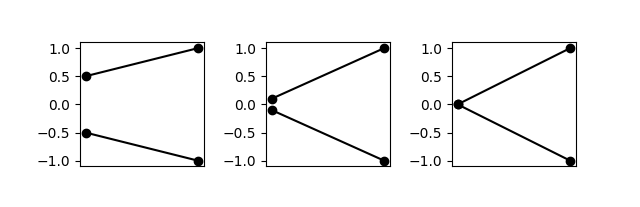
\includegraphics[width=0.8\textwidth]{process_visualization_cropped.png}
    \label{fig:1}
\end{figure}
Tatsächlich hat der Prozess $Y$ (zumindest mit natürlicher Filtration) aber ein vollkommen anderes Verhalten als $X^s$: Bei den Prozessen $X^s$ wird immer schon im ersten Schritt entschieden, zu welchem Pfad sich der Prozess entwickeln wird, wohingegen $Y$ die Entscheidung erst im zweiten Schritt trifft. Während die Wasserstein-Metrik diese Diskrepanz nicht aufzeigen konnte, ist die adaptierte Wasserstein-Metrik dazu in der Lage. Wir können die Methodik aus dem letzten Abschnitt auf die Prozesse $X^s$ und $Y$ mit natürlicher Filtration anwenden und damit die Konvergenz bezüglich $\mathcal{AW}_p$ zu untersuchen. Das Ergebnis ist in Abbildung \ref{fig:0} zu sehen. Es zeichnet sich klar ab, dass $X_s$ nicht gegen $Y$ konvergiert.
\begin{figure}[h]
    \caption{Die adaptierte Wasserstein-Distanz der Prozesse bezüglich natürlicher Filtration. Die Prozesse werden für die Folge $s_n = 2^{-n}$ aufgezeichnet.}
    \centering
    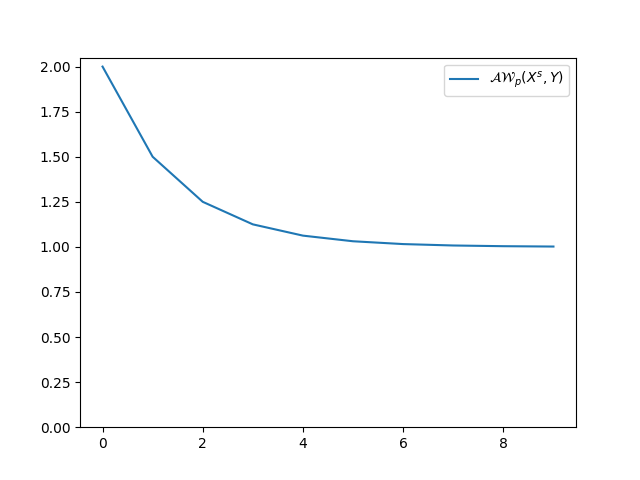
\includegraphics[width=0.7\textwidth]{aw_no_convergence.png}
    \label{fig:0}
\end{figure}

Wie wir besprochen haben ist der Hauptunterschied zwischen den Prozessen der Zeitpunkt der Entscheidung. Diese können wir aber über die Filtration darstellen: Wenn wir beim Prozess $\mathbb{Y}$ auch schon im ersten Schritt die Filtration $\mathcal{F}_1^\mathbb{Y} = \sigma(\{-1\}, \{1\})$ wählen, so sind die Filtrationen der Prozesse identisch. Damit ist die Kopplung $(\id, \id)_* \mathbb{P}$ wieder bikausal und wie bei der Wassersteindistanz konvergiert $\mathbb{X}^s \rightarrow \mathbb{Y}$ für $s \rightarrow 0$. An diesem Beispiel kann man erkennen, wie die adaptierte Wasserstein-Metrik nicht nur Nähe der Verteilungen, sondern auch Nähe des stochastischen Charakters ausdrücken kann.


\section{Appendix}
Die folgende Charakterisierung von bikausalen Kopplungen stammt aus \cite[Lemma A.1]{main_paper}
\begin{lemma} \label{thm:causality_kernel_characterization}
Seien $\mathbb{X}, \mathbb{Y} \in \CFP_p$, $\pi \in \mathcal{P}_p(\mathcal{Z}\times\mathcal{Z})$ und setze $\pi_1 := \operatorname{pj}_{\mathcal{Z}_1\times \mathcal{Z}_1}\pi$. Dann ist $\pi \in \cplbc(\mathbb{X}, \mathbb{Y})$ genau dann, wenn
$$\pi_1 \in \cpl(\mathcal{L}(\ip_1(\mathbb{X})), \mathcal{L}(\ip_1(\mathbb{Y})))$$
und für $1\leq t \leq N-1$ Kerne
$$k_t:\mathcal{Z}_{1:t} \times \mathcal{Z}_{1:t} \rightarrow \mathcal{P}_p(\mathcal{Z}_{t+1} \times \mathcal{Z}_{t+1}) \text{ mit } k_t^{z_{1:t}, \hat{z}_{1:t}} \in \cpl(z_t^+, \hat{z}_t^+)$$
existieren, sodass
$$\pi = \pi_1 \otimes k_1 \otimes ... \otimes k_{N-1}$$
\end{lemma}
\begin{proof}
Da $\mathbb{X}, \mathbb{Y} \in \CFP_p$ können wir die Verteilungen schreiben als $\mathbb{P}^{\mathbb{X}} = \uf_1(\mu)$, $\mathbb{P}^{\mathbb{Y}}=\uf_1(\nu)$ für $\mu, \nu \in \mathcal{P}_p(\mathcal{Z}_1)$.
\begin{enumerate}
\item
Nehmen wir zunächst an, dass $\pi \in \cplbc(\mathbb{X}, \mathbb{Y})$. Dann können wir die Kerne wählen als 
$$k_t = \mathcal{L}_\pi(z_{t+1}, \hat{z}_{t+1} \vert \mathcal{F}_{t,t}^{\mathcal{Z}, \mathcal{Z}})$$
Für diese Wahl gilt $\pi = \pi_1 \otimes k_1 \otimes ... \otimes k_{N-1}$ und mit Lemma \ref{thm:pushforward_law} sind die Marginalien gegeben durch 
$${\operatorname{pj}_1}_*\mathcal{L}_\pi(z_{t+1}, \hat{z}_{t+1} \vert \mathcal{F}_{t,t}^{\mathcal{Z}, \mathcal{Z}}) = \mathcal{L}_\pi(\operatorname{pj}_1(z_{t+1}, \hat{z}_{t+1}) \vert \mathcal{F}_{t,t}^{\mathcal{Z}, \mathcal{Z}}) = \mathcal{L}_\pi(z_{t+1},  \vert \mathcal{F}_{t,t}^{\mathcal{Z}, \mathcal{Z}})$$
und $\mathcal{L}_\pi(\hat{z}_{t+1} \vert \mathcal{F}_{t,t}^{\mathcal{Z},\mathcal{Z}})$. Da $\pi$ bikausal ist, gilt nach Lemma \ref{thm:causality_characterization} 
$$\mathcal{L}_\pi(z_{t+1} \vert \mathcal{F}_{t,t}^{\mathcal{Z,Z}}) = \mathcal{L}_\pi(z_{t+1} \vert \mathcal{F}_{t,0}^{\mathcal{Z,Z}})=\mathcal{L}_{\mathbb{P}^{\mathbb{X}}}(z_{t+1} \vert \mathcal{F}_t^\mathcal{Z})$$
wobei wir für die letzte Gleichheit Lemma \ref{thm:pushforward_expectancy} auf die Projektion auf die erste Koordinate angewendet haben. Aufgrund der Form $\mathbb{P}^{\mathbb{X}} = \uf_1(\mu)$ gilt aber $\mathcal{L}_{\mathbb{P}^{\mathbb{X}}}(z_{t+1} \vert \mathcal{F}_t^{\mathcal{Z}}) = z_t^+$: Dieser Kern ist $\mathcal{F}_t^{\mathcal{Z}}$-messbar, und die induzierte Verteilung ist 
$$\mathcal{L}_{\mathbb{P}^{\mathbb{X}}}(z_{1:t}) \otimes z_t^+ = \mu \otimes z_1^+ \otimes ... \otimes z_{t-1}^+  \otimes z_t^+ = \operatorname{pj}_{1:t+1}(\uf_1(\mu)) = \mathcal{L}_{\mathbb{P}^{\mathbb{X}}}(z_1,...,z_{t+1})$$
Es gilt also $\mathcal{L}_\pi(z_{t+1} \vert \mathcal{F}_{t,t}^{\mathcal{Z,Z}}) = z_t^+$ und analog $\mathcal{L}_\pi(\hat{z}_{t+1} \vert \mathcal{F}_{t,t}^{\mathcal{Z,Z}}) = \hat{z}_t^+$ und somit $k_t^{z_{1:t}, \hat{z}_{1:t}} \in \cpl(z_t^+, \hat{z}_t^+)$.

Nach Bemerkung \ref{thm:ip_of_canonical_process} ist $\mathcal{L}(\ip_1(\mathbb{X})) = \mu = \pj_1(\mathbb{P}^\mathbb{X}) = \pj_1(\pi_1)$. Es gilt also auch $\pi_1 \in \cpl(\mathcal{L}(\ip_1(\mathbb{X})), \mathcal{L}(\ip_1(\mathbb{Y})))$.
\item
Nehme nun umgekehrt an, dass es solche Kerne $k_t$ gibt. Dann ist 
$$\operatorname{pj}_1(\pi) = \operatorname{pj}_1(\pi_1 \otimes k_1 \otimes ... \otimes k_{N-1}) = \mu \otimes z_1^+ \otimes ... \otimes z_{N-1}^+ = \uf_1(\mu) = \mathbb{P}^\mathbb{X}$$
und $\operatorname{pj}_2(\pi) = \mathbb{P}^\mathbb{Y}$ und somit $\pi \in \cpl(\mathbb{X}, \mathbb{Y})$. 

Weiterhin gilt $k_t = \mathcal{L}_\pi(z_{t+1}, \hat{z}_{t+1} \vert \mathcal{F}_{t,t}^{\mathcal{Z,Z}})$, da $\mathcal{L}(z_{1:t}, \hat{z}_{1:t}) \otimes k_t = \mathcal{L}(z_{1:t+1}, \hat{z}_{1:t+1})$. Für ein $\mathcal{F}_{t+1}^\mathcal{Z}$-messbares $U$ gilt dann
\begin{align*}
    \mathbb{E}_\pi(U(z_{1:t+1}) \vert \mathcal{F}_{t,t}^{\mathcal{Z,Z}}) &= \int U(z_{1:t}, z_{t+1}) k_t^{z_{1:t}, \hat{z}_{1:t}}(dz_{t+1}, d\hat{z}_{t+1}) \\
    &= \int U(z_{1:t}, z_{t+1}) z_t^+(dz_{t+1})
\end{align*}
und der letzte Term ist $\mathcal{F}_{t,0}^{\mathcal{Z,Z}}$-messbar. Mit der Turmeigenschaft folgt also für ein $\mathcal{F}_N^\mathcal{Z}$-messbares $U$, dass $\mathbb{E}_\pi\left(U \vert \mathcal{F}_{t,t}^{\mathcal{Z,Z}}\right)$ $\mathcal{F}_{t,0}^{\mathcal{Z,Z}}$-messbar ist und damit Kausalität von $\pi$. Aus Symmetriegründen ist $\pi$ bikausal, also $\pi \in \cplbc(\mathbb{X}, \mathbb{Y})$.
\end{enumerate}
\end{proof}
Der folgende Satz stammt aus \cite[Satz 4.5]{markov_processes_ethier} und charakterisiert separierende Teilmengen von $C_b$ für Verteilungen:
\begin{theorem} \label{thm:separating_measures}
    Sei $(A, d)$ ein polnischer Raum und $M \subset C_b(A)$ eine punktetrennende Algebra, das heißt für $x,y\in A$ existiert ein $f\in M$ mit $f(x)\neq f(y)$. Dann ist $M$ \emph{separierend} für $\mathcal{P}(A)$, das heißt für $\mu, \nu \in \mathcal{P}(A)$ mit
    \begin{equation}\label{eq:A20}
        \mu(f)=\nu(f) \quad \forall f \in M 
    \end{equation}
    gilt $\mu=\nu$.
\end{theorem}
\begin{proof}
    Seien $\mu, \nu \in \mathcal{P}(A)$ mit $\mu(f)=\nu(f)\forall f\in M$. Da $M$ eine Algebra ist, ist auch $H:=\{f+a \vert f \in M, a\in \mathbb{R}\}$ eine Algebra, und Gleichung \ref{eq:A20} gilt auch für $h \in H$. Sei $\varepsilon>0$. Da $(A, d)$ polnisch ist, sind $\mu$ und $\nu$ straff, wir können also kompakte $K_1,K_2 \subset A$ wählen, sodass $\mu(K_1)\geq 1-\varepsilon$ und $\nu(K_2)\geq 1-\varepsilon$. Für das kompakte $K:=K_1\cup K_2$ gilt dann $\mu(K)\geq 1-\varepsilon$ und $\nu(K)\geq 1-\varepsilon$. Sei $g \in C_b(A)$ beliebig. Die Menge $\{h_{\vert K} \vert h \in H\}$ ist eine punktetrennende Algebra und enthält die Funktion $h\equiv 1$. Nach dem Satz von Stone-Weierstraß liegt sie dicht in $C_b(K)$ bezüglich $\|\cdot \|_\infty$. Wir können also $(g_n) \subset H$ wählen mit $\sup\limits_{x\in K} |g_n(x)-g(x)| \rightarrow 0$ für $n\rightarrow \infty$. Für jedes $g_n$ gilt

    \begin{equation}\label{eq:A21}
    \int_A g_n \exp(-\varepsilon g_n^2) d\mu = \int_A g_n \exp(-\varepsilon g_n^2) d\nu
    \end{equation}
    nach dominierter Konvergenz, da 
    $$ g_n \sum_{k=0}^{N} \frac{(-\varepsilon g_n^2)^k}{k!} \rightarrow g_n \exp(-\varepsilon g_n^2)$$
    dominiert durch $\exp\left(\|g_n\|_{\infty}^2\right)$, und die Funktionen auf der linken Seite liegen in der Algebra $H$. Es gilt
    \begin{align*}
        \left| \int ge^{-\varepsilon g^2} \right.&\left.d\mu - \int ge^{-\varepsilon g^2}d\nu \right|  
        \leq \left| \int_S ge^{-\varepsilon g^2}d\mu - \int_K ge^{-\varepsilon g^2}d\mu \right| \\
        &+ \left| \int_K ge^{-\varepsilon g^2}d\mu - \int_K g_ne^{-\varepsilon g_n^2}d\mu \right| 
        + \left| \int_K g_ne^{-\varepsilon g_n^2}d\mu - \int_S g_ne^{-\varepsilon g_n^2}d\mu \right| \\
        &+ \left| \int_S g_ne^{-\varepsilon g_n^2}d\mu - \int_S g_ne^{-\varepsilon g_n^2}d\nu \right| 
        + \left| \int_S g_ne^{-\varepsilon g_n^2}d\nu - \int_K g_ne^{-\varepsilon g_n^2}d\nu \right| \\
        &+ \left| \int_K g_ne^{-\varepsilon g_n^2}d\nu - \int_K ge^{-\varepsilon g^2}d\nu \right| 
        + \left| \int_K ge^{-\varepsilon g^2}d\nu - \int_S ge^{-\varepsilon g^2}d\nu \right| \\
    \end{align*}
    Der 4. Summand auf der rechten Seite ist 0 nach Gleichung \ref{eq:A21}. Die Summanden 1, 3, 5 und 7 sind jeweils beschränkt durch $\gamma \sqrt{\varepsilon}, \gamma:=\sup_{t\geq 0}te^{-t^2}$, da 
    $$te^{-\varepsilon t^2}=\frac{1}{\sqrt{\varepsilon}}(\sqrt{\varepsilon} t)e^{-(\sqrt{\varepsilon}t)^2} \leq \frac{1}{\sqrt{\varepsilon}} \gamma \, \text{ und } \, \mu(S\setminus K), \nu(S\setminus K)<\varepsilon$$
    Die Summanden 2 und 6 konvergieren gegen $0$ für $n\rightarrow \infty$, da $g_n \rightarrow g$ gleichmäßig auf $K$ und $t \mapsto te^{-\varepsilon t^2}$ lipschitzstetig ist, also auch $g_n e^{-\varepsilon g_n^2} \rightarrow g e^{-\varepsilon g^2}$ gleichmäßig auf $K$. Wir erhalten für $n\rightarrow \infty$
    $$\left|\int ge^{-g^2\varepsilon}d\mu - \int ge^{-\varepsilon g^2} d\nu \right|\leq 4\gamma\sqrt{\varepsilon}$$
    Für $\varepsilon \rightarrow 0$ folgt mit dominierter Konvergenz ($g$ und somit $ge^{-\varepsilon g^2}$ sind unabhängig von $\varepsilon$ beschränkt und $ge^{-\varepsilon g^2} \rightarrow g$ punktweise für $\varepsilon \rightarrow 0$), dass
    $$\int gd\mu = \int gd\nu$$

    Sei nun $E \subset A$ abgeschlossen. Für $n\in \mathbb{N}$ sind die Funktionen $g_n: x \mapsto 1 - n \cdot d(x, E)$ stetig und beschränkt, also $\mu(g_n) = \nu(g_n)$ für alle $n \in \mathbb{N}$. Es gilt $g_n \rightarrow \mathds{1}_E$ dominiert durch $1$, mit dominierter Konvergenz gilt also $\mu(E)=\nu(E)$. Abgeschlossene Mengen sind ein $\cap$-stabiler Erzeuger von $\mathcal{B}(A)$, insgesamt folgt also $\mu=\nu$.
\end{proof}

\clearpage
\printbibliography

\end{document}